\documentclass[12pt,a4paper,final]{book}			%definire grandezza testo, foglio e tipo di testo.

\usepackage[svgnames]{xcolor} % Required for colour specification

%				** TIPI DI DOCUMENTI **
%			- article
%			- book
%			- report
%			
%
\usepackage[utf8]{inputenc}			%definisce la codifica dei caratteri
\usepackage[english]{babel}				%definisce il pacchetto della lingua
\usepackage{amsmath}						%contiene molti utili strumenti per la scrittura matematica
\usepackage{amsfonts}
\usepackage{amssymb}
\usepackage{makeidx}
\usepackage{graphicx}
\usepackage{lmodern}
\usepackage{units}  					%unita di misura
\usepackage{pgfplots}				%grafici
\usepackage{subcaption}  		%per le figure
\usepackage{gensymb} 			%per i gradi
\usepackage{pst-solides3d}  %per figure in 3D
%\usepackage{hyperref}				%permette di linkare
\usepackage{circuitikz}			%per circuiti
\usepackage{pgfplots}				%per fare plot pgf
\usepackage{subcaption}		%DON'T KNOW. INVESTIGATE
\usepackage{siunitx} 				%unita SI
\usepackage{wrapfig}				%per mettere più immagini insieme
\usepackage{bbold}					%per avere numeri in \mathbb{}
\usepackage{mathrsfs}			%per usare cose tipo \mathscr{}
\usepackage{physics}				%contiene molta notazione utile; lo uso in particolare per \bra e \ket
\usepackage{pgfplotstable}	%DON'T KNOW. INVESTIGATE
\usepackage{titlesec}				%per formattare titoli, paragrafi etc.
\usepackage{xfrac}
\usepackage{cite}
\usepackage{caption}
\usepackage[font=small,labelfont=bf]{caption}		% serve per ridurre la dimensione delle captions
\usepackage[final]{pdfpages}		%per poter includere pdf

\usepackage[a-1b]{pdfx}
\usepackage[pdfa]{hyperref}
%\usepackage[dvipsnames]{xcolor}	%permette di usare \colorbox. L'argomento del pacchetto è per definire il set di nomi dati ai colori.
%\usepackage{tesi}

%
%
%			FOR CODE SNIPPETS
%
%
\usepackage{listings} % Required for inserting code snippets
\definecolor{DarkGreen}{rgb}{0.0,0.4,0.0} % Comment color
\definecolor{highlight}{RGB}{255,251,204} % Code highlight color
\lstdefinestyle{Style1}{ % Define a style for your code snippet, multiple definitions can be made if, for example, you wish to insert multiple code snippets using different programming languages into one document
language=python, % Detects keywords, comments, strings, functions, etc for the language specified
backgroundcolor=\color{highlight}, % Set the background color for the snippet - useful for highlighting
basicstyle=\footnotesize\ttfamily, % The default font size and style of the code
breakatwhitespace=false, % If true, only allows line breaks at white space
breaklines=true, % Automatic line breaking (prevents code from protruding outside the box)
captionpos=b, % Sets the caption position: b for bottom; t for top
commentstyle=\usefont{T1}{pcr}{m}{sl}\color{DarkGreen}, % Style of comments within the code - dark green courier font
deletekeywords={}, % If you want to delete any keywords from the current language separate them by commas
%escapeinside={\%}, % This allows you to escape to LaTeX using the character in the bracket
firstnumber=1, % Line numbers begin at line 1
frame=single, % Frame around the code box, value can be: none, leftline, topline, bottomline, lines, single, shadowbox
frameround=tttt, % Rounds the corners of the frame for the top left, top right, bottom left and bottom right positions
keywordstyle=\color{Blue}\bf, % Functions are bold and blue
morekeywords={}, % Add any functions no included by default here separated by commas
numbers=left, % Location of line numbers, can take the values of: none, left, right
numbersep=10pt, % Distance of line numbers from the code box
numberstyle=\tiny\color{Gray}, % Style used for line numbers
rulecolor=\color{black}, % Frame border color
showstringspaces=false, % Don't put marks in string spaces
showtabs=false, % Display tabs in the code as lines
stepnumber=5, % The step distance between line numbers, i.e. how often will lines be numbered
stringstyle=\color{Purple}, % Strings are purple
tabsize=2, % Number of spaces per tab in the code
}

\lstdefinestyle{Style2}{ % Define a style for your code snippet, multiple definitions can be made if, for example, you wish to insert multiple code snippets using different programming languages into one document
language=bash, % Detects keywords, comments, strings, functions, etc for the language specified
backgroundcolor=\color{highlight}, % Set the background color for the snippet - useful for highlighting
basicstyle=\footnotesize\ttfamily, % The default font size and style of the code
breakatwhitespace=false, % If true, only allows line breaks at white space
breaklines=true, % Automatic line breaking (prevents code from protruding outside the box)
captionpos=b, % Sets the caption position: b for bottom; t for top
commentstyle=\usefont{T1}{pcr}{m}{sl}\color{DarkGreen}, % Style of comments within the code - dark green courier font
deletekeywords={}, % If you want to delete any keywords from the current language separate them by commas
%escapeinside={\%}, % This allows you to escape to LaTeX using the character in the bracket
firstnumber=1, % Line numbers begin at line 1
frame=single, % Frame around the code box, value can be: none, leftline, topline, bottomline, lines, single, shadowbox
frameround=tttt, % Rounds the corners of the frame for the top left, top right, bottom left and bottom right positions
keywordstyle=\color{Blue}\bf, % Functions are bold and blue
morekeywords={}, % Add any functions no included by default here separated by commas
numbers=left, % Location of line numbers, can take the values of: none, left, right
numbersep=10pt, % Distance of line numbers from the code box
numberstyle=\tiny\color{Gray}, % Style used for line numbers
rulecolor=\color{black}, % Frame border color
showstringspaces=false, % Don't put marks in string spaces
showtabs=false, % Display tabs in the code as lines
stepnumber=5, % The step distance between line numbers, i.e. how often will lines be numbered
stringstyle=\color{Purple}, % Strings are purple
tabsize=2, % Number of spaces per tab in the code
}
% Create a command to cleanly insert a snippet with the style above anywhere in the document
\newcommand{\insertcode}[2]{\begin{itemize}\item[]\lstinputlisting[caption=#2,label=#1,style=Style1]{#1}\end{itemize}} % The first argument is the script location/filename and the second is a caption for the listing

\newcommand{\insertbash}[2]{\begin{itemize}\item[]\lstinputlisting[caption=#2,label=#1,style=Style2]{#1}\end{itemize}} 








%TITOLO


% NOT SURE WHAT THIS DOES. IT WAS PRESENT IN GABRIELE'S TEXT
\makeatletter
\renewcommand*\env@matrix[1][\arraystretch]{%
  \edef\arraystretch{#1}%
  \hskip -\arraycolsep
  \let\@ifnextchar\new@ifnextchar
  \array{*\c@MaxMatrixCols c}}
\makeatother
% ----------------------------------------------------- % 
% ----------------------------------------------------- % 
% ----------------------------------------------------- % 
% ----------------------------------------------------- % 
\title{
		\centering
		\vspace{2mm}
		\begin{figure}[h]
			\centering{
			
\includegraphics{figures/logo.jpg} }
		\end{figure}
		 \vspace{5mm}
		 {FACOLTÀ DI SCIENZE E TECNOLOGIE} \\
		 {DIPARTIMENTO DI FISICA ALDO PONTREMOLI} \\
		 {Corso di Laurea triennale in Fisica (L-30)} \\
		 \vspace{5mm}
		\noindent\hrulefill \\
		\vspace{5mm}
		 \textbf{{Glitches classification in the Plank/HFI experiment using neural networks.}} 
	 }
% ----------------------------------------------------- % 
	 
	\date{11 October 2019}
\begin{document}

%
%
%			TITLE
%
%


\includepdf[pages=-]{TITLEPAGE/titlepage_thesis.pdf}
		
\newpage
\thispagestyle{empty}
\clearpage\mbox{}\clearpage

\newpage
\thispagestyle{empty}
\tableofcontents

\newpage
\thispagestyle{empty}
\clearpage\mbox{}\clearpage

\newpage

\chapter{The Cosmic Microwave Background}\label{intro_CMB}
		In this chapter I briefly outline the astrophysical background behind the work done in this thesis. I describe what the Cosmic Microwave Background is and its measurement by experiments like Planck. 
		
	\section{The CMB and the Universe}\label{general_information}
		 The present Universe, according to the \textbf{Standard Model of Cosmology}, began approximately $14$ billion years ago from a mathematical singularity named \textbf{Big Bang}. In its early stages, spacetime underwent a very rapid period ($10^{-33}~\unit{s}$) of expansion, known as \textit{Inflationary Period}, followed by a slower and more regular expansion. In this early phase, matter and radiation were in equilibrium in a hot plasma that progressively cooled down as the expansion went on.
			
			By $10~\unit{s}$, protons and neutrons were formed; Helium nuclei were produced shortly after. Radiation-matter equilibrium\footnote{This was due to the so-called \textit{Thomson scattering} between photons and electrons.} ended when the temperature reached $T \simeq 3000~\unit{K}$, permitting the formation of neutral atoms. When this happened, matter and radiation decoupled: most of the electrons were captured by atomic nuclei, thus not allowing any more interactions with traveling photons, which were free to propagate. This happened about $380~000~\unit{yr}$ after the formation of the Universe. After billions of years, today these primordial photons are still moving through space.
			\begin{figure}[h!]
				\centering
				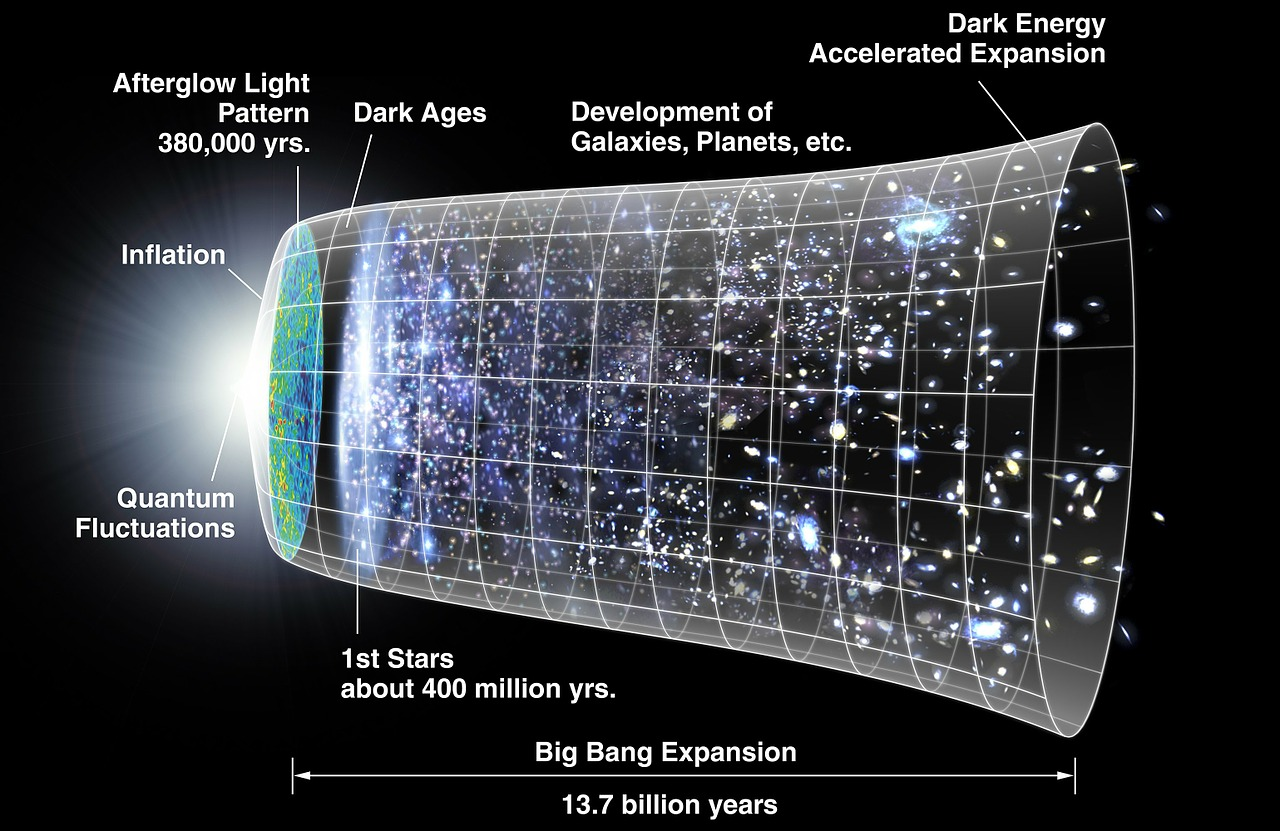
\includegraphics[scale=0.3]{figures/universe_history.jpg}
				\caption{Visual representation of the evolution of the Universe, according to the \textit{Cosmological Standard Model}.}
				\label{universe_history}
			\end{figure}						
			
			The spectrum of the primordial radiation is a perfect black body. 
			 Over billions of years, as a result of the expansion of the Universe, the temperature of this blackbody has decreased to $2.7~\unit{K}$, with a peak emission of $1~\unit{mm}$, in the \textit{microwave} range. These photons have been detected for the first time in 1964: since then, they have been known as the \textbf{Cosmic Microwave Background} (CMB). 
%			 Their blackbody temperature, from the initial value of around $3000~\unit{K}$, has dropped to just $2.7~\unit{K}$, which makes its measurement quite an engineering challenge.
			 
%			 \textbf{An important concept in CMB studies is the \textbf{spectral density}. Its role is to depict the distribution of power into frequency components of a signal. In case of photons measurements, as the ones that have to be carried out to detect the Cosmic Background, its form is essential in identifying which frequencies is best to probe. Fig \ref{fig:Tomasi_spectral_density} shows the spectral density of the sky. The CMB is not the only signal present and it dominates in only a small frequency range. Most of the other effects present are related to the \textit{Galactic Magnetized Interstellar Medium} (ISM). The study and modelling of such components is of valuable importance in the study of the CMB. \cite{synchrotron_emission}}

		In case of a non-expanding Universe, the primordial photons we can see from Earth are those that were at a distance $c(t_{now} - t_{dec})$, where $t_{dec}$ is the time of decoupling.
			 This means that an observer on our planet can only see a spherical shell of photons, called \textbf{Last Scattering Surface} (LSS). 
			 If one takes into consideration the expansion, as it is actually true for our Universe, the idea behind it is the same, but with more mathematical complexity.
			 To measure the properties of the CMB (or any scalar field), it is common to use a decomposition in \textit{spherical harmonics}. For a given function $f(\theta, \varphi)$ on a sphere (the LSS in the case of CMB), its decomposition is:
			\[
				f(\theta, \varphi ) = \sum_{\ell = 0}^{\infty} \sum_{m = -\ell}^{\ell} a_{\ell m} Y^{m}_{\ell} (\theta, \varphi)
			\]
			where $Y^{m}_\ell$ are the spherical harmonics and $a_{\ell m}$ are some complex coefficients. Without too much detail (see \cite{Libro_CMB}), it can be shown that $\left|a_{\ell m }\right|^2$ quantifies the perturbations in the function $f$ for a given angular scale. In cosmology, it is useful to define the quantity \textbf{power spectrum} as:
			\[
				C_{\ell} = \left \langle a_{\ell m } a^*_{\ell m } \right \rangle
			\]
			where, in case of data measured by a single instrument, the average is done over all possible values of $m$.
			 
			 The Standard Model of Cosmology is based on an \textit{inflationary paradigm} to explain the great homogeneity present in the CMB as observed today. The theory predicts that points very close to one another were distanced by the inflation. 
%			 large scale differences present in the Universe as observed today. 
%			 This theory predicts that small quantum fluctuations, enlarged by the inflation, became large scale cosmological structures.
\cite{b_modes_tomasi}
 A prediction of this paradigm is a background of \textit{Gravitational Waves} (GW), generated by quantum fluctuations, to be expanded macroscopically. The difficulty in the study of \textbf{primordial GW} arises from their long wavelengths, which make their detection through some GW interferometers, e.g. LIGO,  impossible.
			 
			During the matter-radiation equilibrium dominated by \textit{Thomson scattering}, some radiation can be polarized. If a radiation field possesses a \textit{quadrupolar} component, it can produce different types of polarization. These can be recorded through the measurement of some specific patterns, called \textbf{E-modes} and \textbf{B-modes}. It can be shown that gravitational waves can only produce the latter, while E-modes are due to adiabatic pressure oscillations (sound waves) and vorticity in the velocity field in the primordial plasma. 
			
%			It can be shown that a decomposition into spherical harmonics holds true for vector and tensor fields. 
			A decomposition in spin-weighted spherical harmonics permits to define a power spectrum for vector and tensor fields as well.
			In case of sound and gravitational waves, this mechanism is at the basis of distinction between E and B-modes. It is then possible to associate a power spectrum to the two polarization patterns: to prove the existence of relic GW in the Universe it would be sufficient to measure the power spectrum for B-modes. Fig. \ref{fig:Tomasi_power_spectrum} shows the power spectrum for different components of the CMB. The power of B-modes is significantly smaller than that of the temperature or that of E-modes. In cosmology, the parameter $r$ is defined as the ratio between the power of primordial B-modes and that of E-modes. In the image, two scenarios for different $r$ are shown.

			 \begin{figure}[h!]
			 	\centering
			 	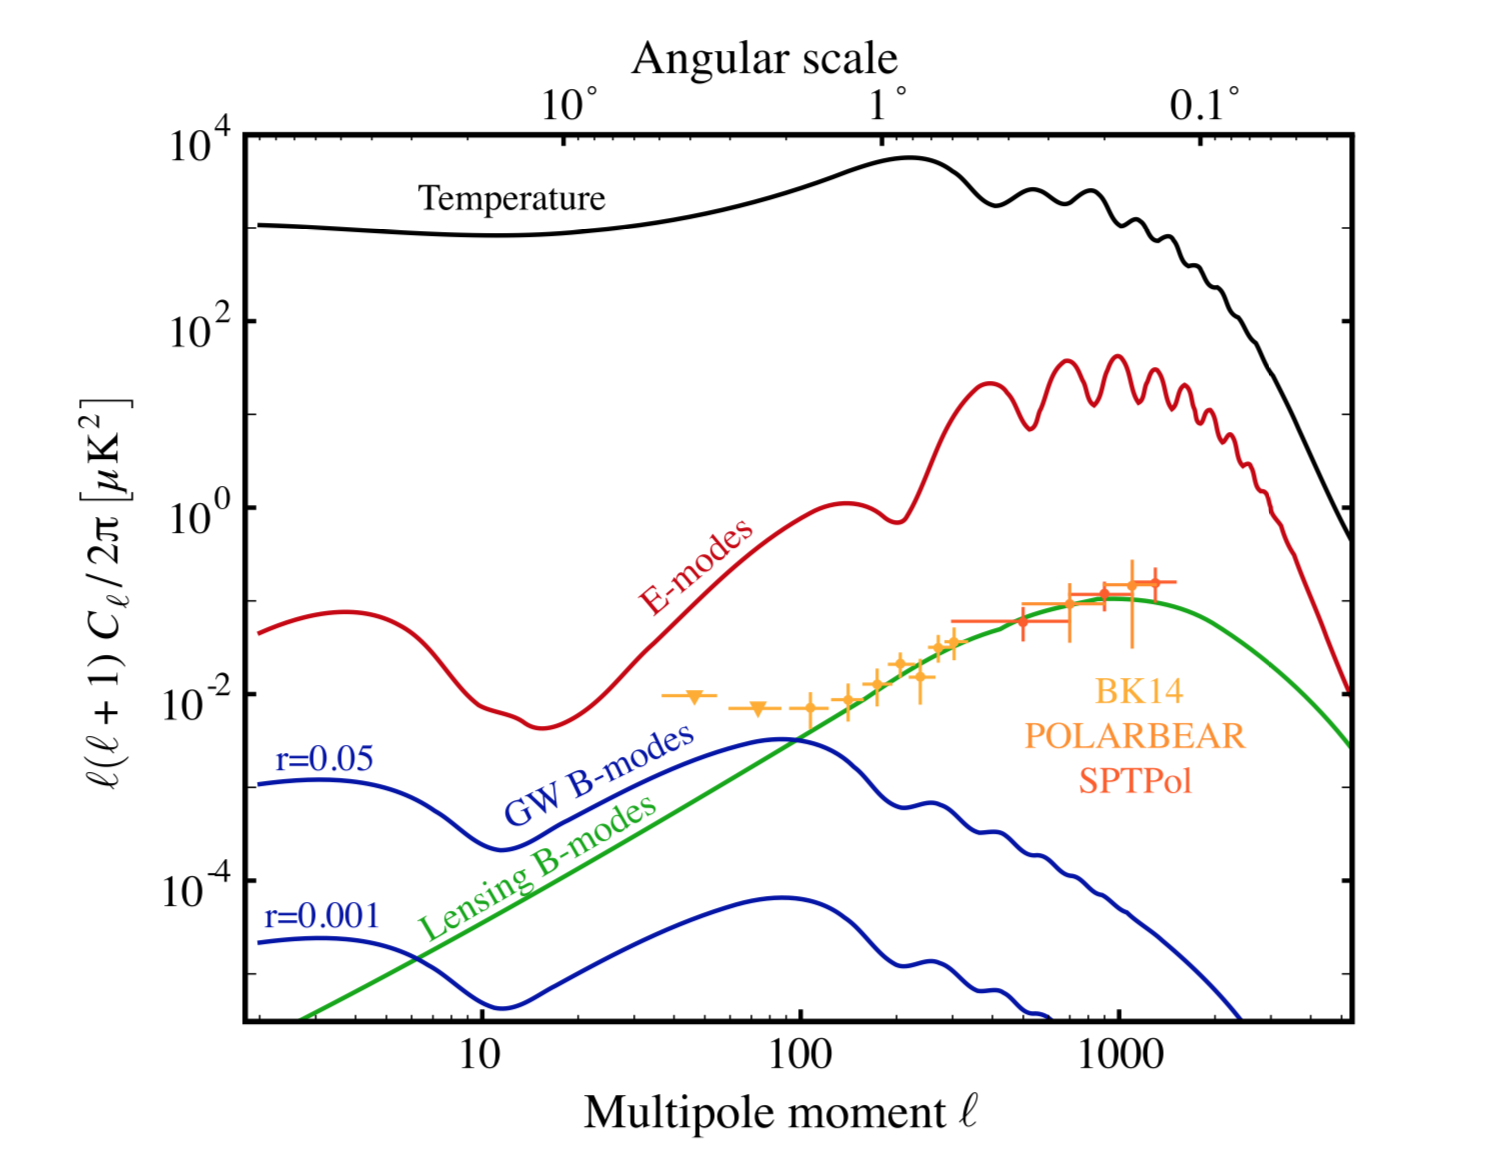
\includegraphics[scale=0.5]{figures/power_spectrum.png}
			 	\caption{Power spectra predicted for temperature, E-modes and B-modes. The primordial B-mode spectrum is by far the faintest. So far, only some measurements of lensing B-modes have been accomplished. \cite{Libro_CMB}}
			 	\label{fig:Tomasi_power_spectrum}
			 \end{figure}
			 
			 Over the years, many experiments have been measuring the CMB. After many ground-based instruments, the first space mission was the \textbf{Cosmic Background Explorer} (COBE), launched by NASA in 1989, which made the first detection of the temperature fluctuations in the CMB across the sky. In 2001, NASA launched a second-generation mission, \textbf{Wilkinson Microwave Anisotropy Probe} (WMAP), which measured the differences across the sky in temperature, leading to the estimation of important cosmological parameters, e.g. the age of the Universe, its total density, Hubble's constant and many others.\cite{WMAP} The latest of CMB missions, Planck, was launched in 2009 by the European Space Agency. 
			 
			\begin{figure}[h!]
				\centering
				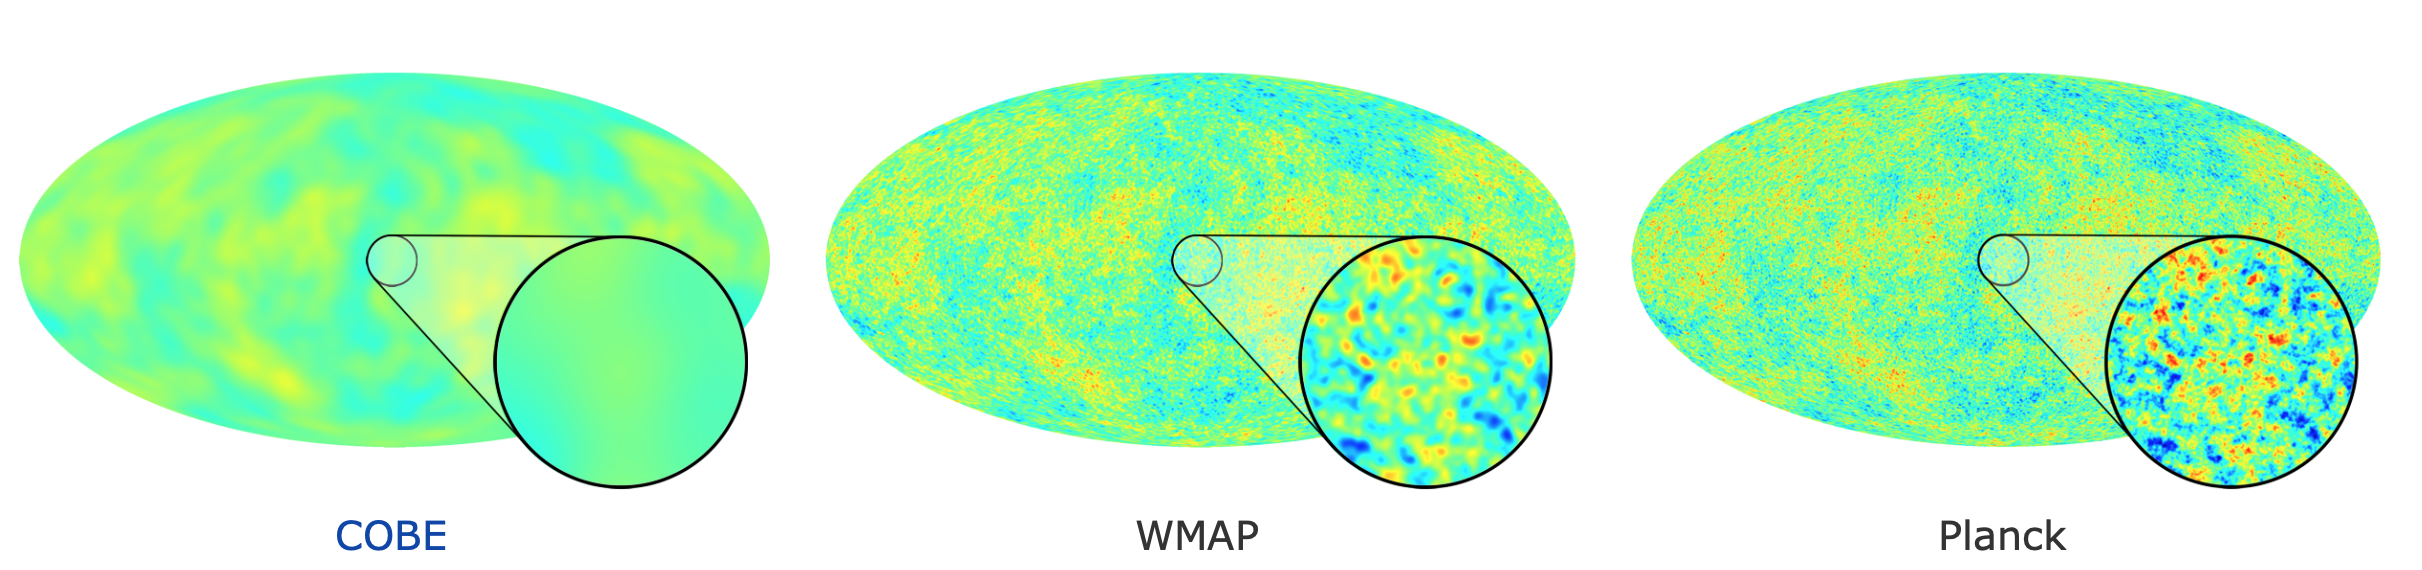
\includegraphics[scale=0.35]{figures/detail_missions_cmb.png}
				\caption{Detail in the measurement by the three generations of CMB missions. Credits: \textit{Chris North, Cardiff University}.}
				\label{detail_cmb}
			\end{figure}						 
			
			Theoretically, the microscopical patterns generated by Primordial Gravitational Waves, due to the expansion of the Universe, can be measured. Observing GW B-modes is today of extreme importance, since it would be a direct evidence for the \textit{Inflationary Period}. A difficulty in this regard is given by \textbf{gravitational lensing}: this effect does not create new photons, but modifies the polarization patterns in the deflected radiation. This means that pure E-modes photons, when affected by a gravitational wheel, become a mix of E and B. This effect has a very broad range in angular scales, but it peaks at high multipoles, substantially smaller angular scales than what is predicted for GW B-modes. In order to detect primordial B-modes polarization, it is necessary to use a procedure called \textbf{delensening} to clean CMB maps.
			 
			  
		\section{Plank/HFI experiment}\label{planck_experiment}
		
			The Planck satellite was launched by the European Space Agency (\textbf{ESA}) in May 2009 to make high sensitive measurements of the sky signal in the frequency range $30–850~\unit{GHz}$, with the purpose of measuring the CMB anisotropies after having separated them from the Galactic and extragalactic contamination. The Plank collaboration published its most accurate results in 2018. \cite{planck_overview}
			
			The Planck experiment is, to date, to most important satellite deployed to study the CMB: it allowed for evaluations of the background temperatures with precisions of up to $1$ part per million.
			The satellite itself was positioned with a Lissajous orbit around $L_2$ (Sun-Earth second Lagrangean point), in order to always be aligned along the Sun-Earth axis for the duration of the experiment. 			
			
			The satellite carried two experiments, which made measurements in separate frequency ranges:
				\begin{itemize}
					\item LFI (\textit{low frequency instrument}) probed the sky at $30$, $44$ and $70$ $\unit{GHz}$ range. It deployed pseudo-correlation differential receivers based on HEMT technology, kept at an operating temperature of $20 ~\unit{K}$.
					\item HFI (\textit{high frequency instrument}) measured frequencies in the range between $100$ and $857~\unit{GHz}$. It implemented 48 bolometers working at $0.1~\unit{K}$.
				\end{itemize}
				In this thesis, my focus will be only on \textbf{HFI} and the data it produced. I will then explain hereafter, in more detail, how it worked and how it collected data.\cite{tesi_tomasi}					
				
				HFI consisted of 48 bolometers, making up 52 total receivers that probed the $100–857~\unit{GHz}$ range in six bands. These bolometers can be approximated to a blackbody-like grid that absorbs the radiation coming from the satellite mirrors and, thus, heats up. This variation in temperature is measured, for each position in the sky, using a solid-state thermometer. 
				Some of the bolometers were also able to measure radiation polarization of light, but its discussion exceeds the aim of this thesis.
				To keep the bolometer at working temperature of $0.1~\unit{K}$, three cooling stages were implemented on-board the spacecraft.
		\section{Cosmic Ray Glitches}\label{cosmic_ray_glitches}
			While the satellite is in outer space, orbiting around the Sun, it is continuously hit by \textbf{cosmic rays}. Even though different types of shields are present to insulate the detectors as best as possible, some form of unwanted radiation manages to trigger a spurious signal in the receivers.
			While \textit{LFI} used microwave radiometers to probe the sky, \textit{HFI}, which, as said, was comprised of bolometers kept at a very low temperature, was way more sensitive to cosmic rays. Indeed, a single cosmic ray can leave a trace in the thermometers many times the size of the background, which is around $2.7~\unit{K}$.
			These signals are labeled as \textbf{glitches}, and the purpose of this work is to develop algorithms to detect them in the raw data of the satellite. 
									The Planck collaboration has managed successfully to exclude such glitches from their analysis, through the use of algorithms based upon \textit{rms} threshold. \cite{planck_glitches}
									
									I will briefly outline the many types of glitches that characterize Planck/HFI unusually high rate ($1~\unit{s^{-1}}$).
						 Generally, glitches can be classified into 3 distinct classes: \textit{short}, \textit{long} and \textit{slow}. Even though most of the times these can be differentiated easily, the three classifications are purely fictional and some events can fall in between.			
				\begin{figure}[h!]
					\centering
					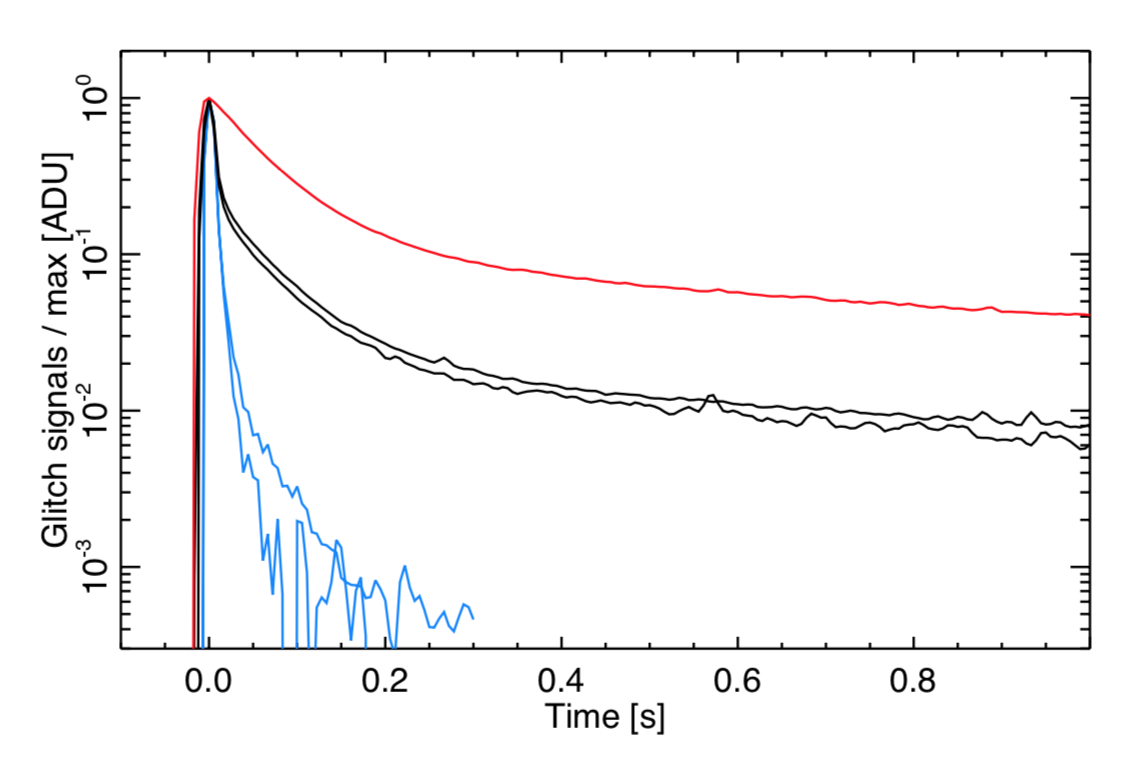
\includegraphics[scale=0.5]{figures/plagio_glitches.png}
					\caption{Examples of the three families of glitches for a typical bolometer. The blue curve represents \textit{short glitches}, the black \textit{long} and the red \textit{slow}. Their \textit{rise time} is defined as the time it takes to reach their respective maximum value, which is, as shown, comparable with the sampling time of HFI. \cite{planck_glitches}}
					\label{plagio_glitches}
				\end{figure}
				
				The \textbf{short glitches} family consists of events that have a rise time of around or less than $5~\unit{ms}$, which is the sampling time of the instruments. This means that sometimes the value registered by the thermometer is not exactly the total amount of energy absorbed by the bolometer. They also present a very fast decay (the same order of magnitude as the rise) and a tail with a value of a few percentage points of its maximum. This family of glitches, probably, arises from the direct interaction of high energy particles with the grid of the bolometers. 		\cite{glitch_impact_planck}			
				
				\textbf{Long glitches} have a rise time similar to that of \textit{short glitches}, but its decay time is around $10$ to $100$ times the sampling time of the instruments. The main distinct feature of this family is the presence of a much larger tail (approximately $50\%$ of its maximum value at half the decay time).
				
				\textbf{Slow glitches} have a higher rise time than \textit{long glitches}, but they present a similar pattern for the tail and decay time. They are the most rare of the three families of glitches (around a few per hour) and their origin is still up to debate, due to relative little experiments in their regard. 	
			
		\section{Beyond Planck}
			
			Present and future missions, both ground based and using space satellites, aimed at advancing the knowledge about the CMB, especially its polarization. I report here the most prominent ones, active or scheduled:
			\begin{itemize}
				\item POLARBEAR and Simons Arrays. A series of receivers that aims at characterizing the arc-minute angular scale B-modes signal from weak gravitational lensing and search for the degree angular scale of primordial GW B-modes. They operate from the Chilean Atacama Desert.\cite{POLARBEAR} 
				
				\item BICEP and Keck Array. The mission has so far consisted of $4$ generations of detectors aimed at measuring, in the $95–150~\unit{GHz}$ range, the presence of B-modes in the CMB polarization. The next generation of receivers, called \textit{BICEP array}, should start observing in the 2020 season and will be comprised of over $30,000$ detectors. This experiment is based in Antartica. \cite{BICEP}
				
				\item South Pole Telescope (SPT). Its 10-meter diameter telescope is designed to probe the sky in the millimeter-wavelength region. It has allowed for the survey of clusters of galaxies and for very accurate measurements of the CMB anisotropies. The first gravitational lensing B-mode signal has been detected by this mission in $2012$. It is located in Antartica. \cite{SPT}
				
				\item Adv-ACT. Located in the Atacama Desert, it is the highest permanent telescope in the world. It works en-pair with other missions, like SPT and BICEP, to study CMB anisotropies and lensing B-modes.
				
				\item Cosmology Large Angular Scale Surveyor (CLASS). The experiment measures the signal from primordial GW in the polarization of the CMB. Just like POLARBEAR and Adv-ACT, it is located in the Atacama Desert. \cite{CLASS}
				
				\item The Large Scale Polarization Explorer (LSPE). It is composed of 2 instruments: a balloon high frequency and a ground based low frequency instrument, which will measure polarization modes at large angular scales in the CMB. It will also give measurements for the creation of a map of foreground polarization. The balloon will perform a long duration flight ($2$ weeks) in the Arctic regions. \cite{LSPE}
				
				\item ALI. A ground based mission comprised of two telescopes built in the Tibetan Plateau. It will aim at measuring CMB B-modes polarizations in the northern hemisphere and give data complementary to Antarctic and Atacama based missions. \cite{ALI}
				
				\item QUBIC. Located in Puma de Atacama, Argentina, it deploys new \textit{Bolometric Interferometers} to study B-modes polarization in the CMB. \cite{QUBIC}
				
				\item \textbf{CMB-S4}. One of the most important ground based experiments that will observe, with dedicated telescopes operating from the South Pole, the Chilean Atacama plateau and, possibly, northern hemisphere sites, B-modes in the CMB radiation.\footnote{For more information regarding the advancement of the mission, see \texttt{https://cmb-s4.org}.}
				
				\item \textbf{LiteBIRD}. This is the fourth generation of space missions aimed at studying the Cosmic Microwave Background. It will observe the sky in the $40–400~\unit{GHz}$ for 15 bands and subtract foregrounds. The $2,622$ detectors will be bolometric-technology based and kept at milli-Kelvin temperatures. Its main goal is to target B-mode polarization patterns in the CMB for one degree or more. It will be launched by the \textit{Japanese Space Agency} (JAXA) in 2027. \cite{LiteBIRD}
			\end{itemize}
			
				
	\chapter{Neural Networks for classification}\label{machine_learning}
		In this chapter I describe what Machine Learning is and which specific class of ML algorithms I have deployed for this thesis.	

		\section{Machine Learning}	
		\textbf{Machine Learning} is a term used to refer to a series of algorithms and techniques that improve their performance through experience. In case of a computer, experience usually means a set of multiple tests aimed at refining how the machine works on a specific problem. The first type of programs written using this idea have began appearing in the late '50s, but only recently, mostly due to advancements in computing power, they have become mainstream.		
		
		In this thesis, I work with an algorithm based upon this premise: through many cycles, I train a program in order to recognize when a timeseries contains a glitch or not. I will first outline some general ideas about the theory behind it.		
		
		Machine Learning provides a powerful tool to analyze large datasets and build upon them. Even though the term is general and comprises many different algorithms, some features are present in every situation it is deployed. 
		First of all, it is \textit{accurate}: these techniques arise from finding, through many trials, the correct optimal decision-making engine for a specific problem. This accuracy scales with the amount of data used: the more information is given to the system, the better it will find the \textit{correct} way.
		ML algorithms are \textit{automated}, where the ``human part" consists only in building the outline and letting the computer learn on its own. Most of these techniques tend to be very fast, compared to more traditional approaches, and they are \textit{customizable}: most data driven problems, even though in completely different areas and contexts, can be solved through the application of Machine Learning. 		
		
	When applied, ML techniques can vary enormously in complexity, both on the ``learning" side as well as finding a way to work with the data at hand. Indeed, most of the work involved around Machine Learning is centered around preparing the data one has in a way that is feedable to the program chosen. Another task is to formulate the problem in a way that ML can be deployed, and this can be in itself a big endeavour. All of these problems can be classified into the term \textit{feature engineering}: to transform the input into something that can be used to learn is the core of Machine Learning. 
		\cite{brink}
		
		\section{Neural Networks}\label{neural_net}
			Within the realm of Machine Learning, there exists a big subfield that, in recent years, has gained much attention and has allowed for advancements in the artificial intelligence field: \textbf{Neural Networks}. 
			The name may sound complicated, but it just stands for the idea of having successive \textit{layers} of representation unto which some algorithm learns. 			 
			These \textit{layers} are usually stacked one on top of the other, in a web-like interface, which can resemble the way neurons are connected to one another.\footnote{I would like to emphasize how the term \textit{neural} does not mean, in any way, that this class of algorithms take examples from the structure of the brain.}
			
			This specific class of algorithms is at the center of my study: using a particular type of neural network, I undertook the task to recognize glitches inside Planck/HFI data. 
			
			When many layers are applied to a \textit{neural network}, it is conventional to call it \textit{Deep Neural Network}. In such instance, it belongs to the subfield of \textbf{Deep Learning}.
			
			%I will briefly outline the functioning, in general, of a neural network, before going into detail on the type that I have used in this work.			
			
			The best way to think about a neural network model is as a multistage information breakdown, where each stacked filter purifies the data it is given until a final output is produced. The algorithm then changes some parameters present inside the model in order to obtain a better result, and the process is repeated. After a series of \textit{epochs}, it will reach some convergence. Fig. \ref{sketch_plagio} shows a representation of a neural network made up of 2 layers. Some form of input, e.g. data from the satellite, is given to the first layers, which, through some algebrical operations depending on some values (\textit{weights}), transforms the data. A second layer follows, which outputs a value for a prediction, $Y^\prime$, constructed in a manner that it can be confronted to a target value, $Y$. As shown in Section \ref{network_training}, in the case of data from Planck/HFI, a simple flag ($0$ or $1$), signaling whether there is a glitch or not, can be used to compare: in such case, the network must be built as to have a similar output as the flag. 
			
			The \textbf{loss function} has the task to confront the output with the desired result and give a score, which will be used by the network to modify the weights. 
						The central task in a neural network is to find a way to tell the net how to improve its result depending on the \textit{loss score}: that is done through the \textit{optimizer}, a function that implements a \textbf{backpropagation algorithm}. Its job is to adjust the weights in order to lower the loss. 
			\begin{figure}[h!]
			\centering
				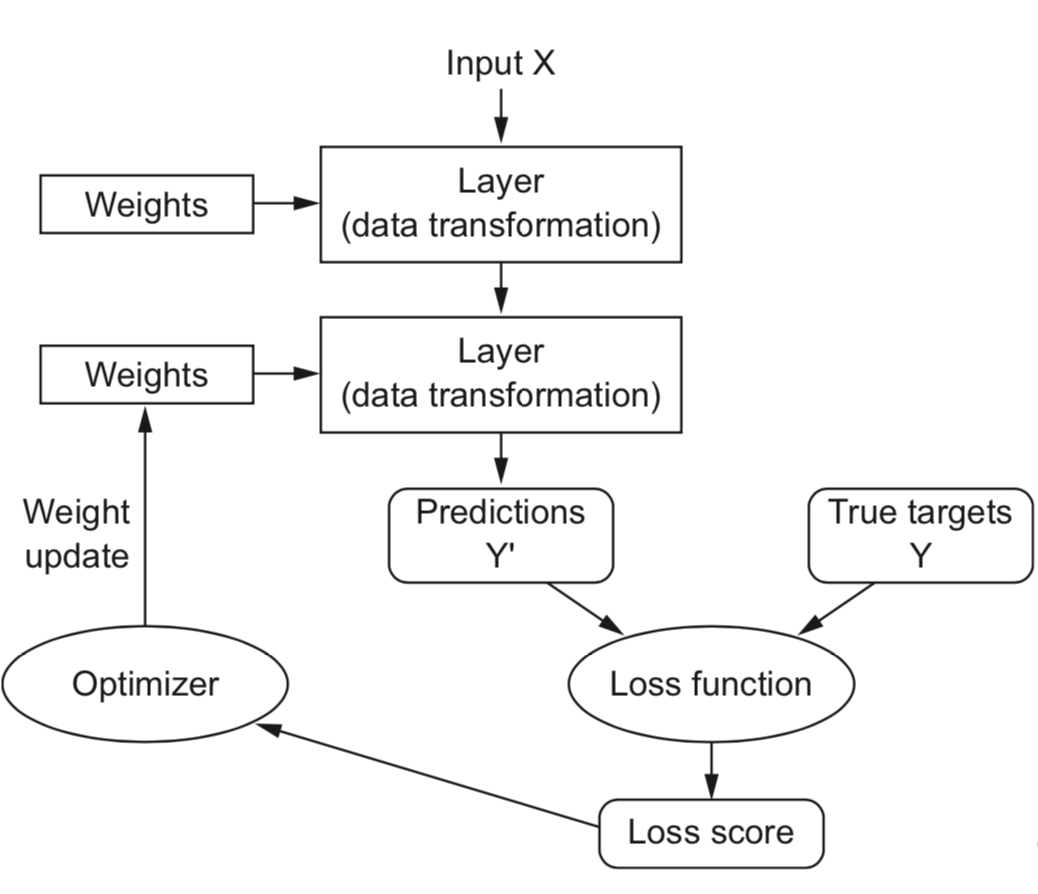
\includegraphics[scale=0.5]{figures/plagio_neural_network.png}
				\caption{Simple sketch of a neural network with 2 layers. Image from Chollet's \textit{Deep Learning with Python}.}
				\label{sketch_plagio}
			\end{figure}						
									
			What happens is as follows:
			\begin{itemize}
				\item The network is built according to the problem faced. In this instance, some random values are assigned to the weights in each layer: this means that, on the first iteration, the operations the data is submitted to are purely random.
				\item A score is computed: given the fact that the process has, so far, been completely random, the result will be far from the desired output, and the loss will be high.
				\item The optimizer decides which way is ``better" to go, and, through the backpropagation, slightly modifies the weights.
				\item The process is repeated many times, until some values for the weights are generated as to minimize the loss. This process is called \textit{training loop}.
			\end{itemize}
			Once scaled to account for thousands of examples and tens of iterations, neural networks have proven to be a remarkable tool for many cases. Its applicability to a large variety of problems has led me to chose this approach and see how it could fare when applied in an astrophysical scenario.\cite{chollet}			
		\section{Convolutional Networks}\label{convnet}
			Among the many choices that one could make regarding the structure of a neural network, I picked \textbf{Convolutional Neural Networks}, also known simply as \textit{convnets}. Their main field of application has been, from their invention, that of computer vision. The feature that makes this network model so successful is due to the way it learns from a set of data: while other types of neural networks learn global patterns from a given input, convnet learn local patterns. 
			
			The ability to learn local characteristics means that convnets are \textit{translationally invariant}. If a network learns a certain pattern in a specific region of the data, it will be able to recognize it anywhere else. 
			In case of HFI glitch recognition, this ability to find a pattern anywhere in the data has been a key feature in my decision to use them. Indeed, when I randomly take a sample of $100$ points from the recorded data, the position of a possible glitch would itself be random. Without \textit{translational invariance}, the task would have been more complicated, although there are techniques to mitigate this problem.
			
			Another important property of convolutional networks is \textit{hierarchical spatial learning}. This means that, when stacking multiple convolutional layers, every step will learn a different feature, each more specific the more it is processed. Fig. \ref{plagio_gatto} shows an example of hierarchical learning in a case of image recognition of a cat: every successive layer learns more specific features from the image. 
			\begin{figure}[t]
				\centering
				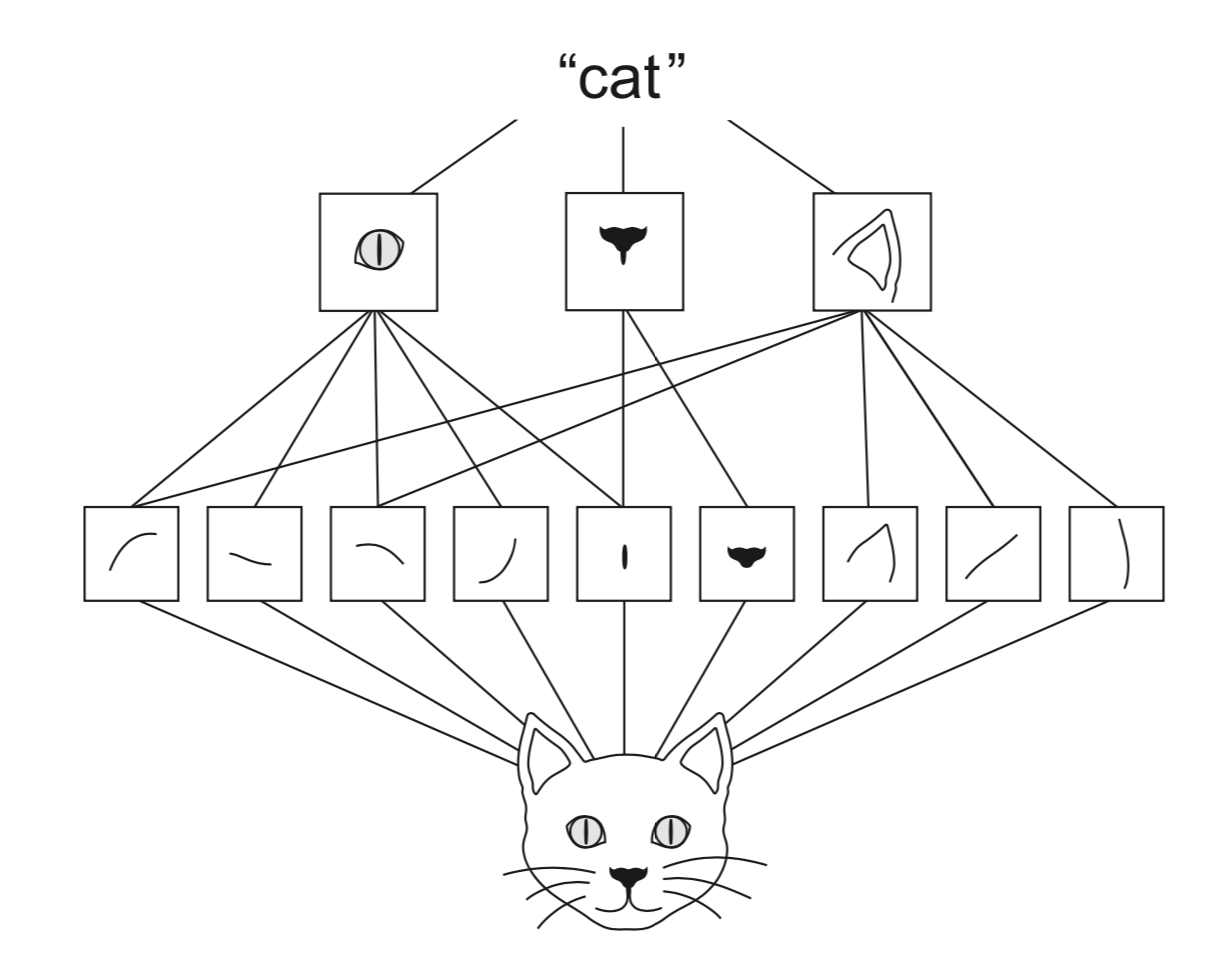
\includegraphics[scale=0.4]{figures/plagio_gatto.png}
				\caption{A visualization of the process of learning in case of a cat image recognition. The second layer learns more specific objects from the first one. Image from Chollet's \textit{Deep Learning with Python}.}
				\label{plagio_gatto}
			\end{figure}
			
			In my specific case, the type of convolutional operations that I decided to work with are called \textit{one dimensional} (1D). They are designed to extract local patches from a time sequence, which is the main reason I decided to apply it. Such type of network is constructed in order to take as input a 3D tensor, whose axes represent the \textit{number of samples}, the \textit{time} and the \textit{number of features}. 
%			What the 1Dconvnet does is take the time axes and select a specific window, set and optimized by me (see Section \ref{optimization_of_the_network_parameters}), onto which it will do some sort of operations, e.g. dot product with weights. 
%			This operation can be done multiple times, through the use of many layers. 
			
			
%
%
\chapter{Glitch Classification}\label{glitch_classification}
\label{data_preparation}

In this chapter I specify what I did to clean the raw data from Planck/HFI and they way I prepared it for the training procedure.

	\section{Data preparation} \label{data_preparation}
		In order to train any neural network, some preparation and classification on raw data is needed. In my enterprise, the data from the Plank/HFI instruments were not ready to be used right away. Even before being able to classify them by hand, I addressed the following problems:
		\begin{itemize}
			\item Contamination in the signal measured in the timelines by the Milky Way dust.
			\item Modulation of the timelines caused by the CMB Dipole.
		\end{itemize}
		In this chapter I explain the aforementioned phenomena.
		
		\subsection{Milky Way dust} \label{Milky_way}
		
		As the satellite spins, it can happen that the telescope is pointing towards the Galactic Plane. In this case, most of the signal is due to emissions from the \textit{Interstellar Medium}. This alters the shape of the timelines in a manner that could hinder the detection of glitches.
		
		In order to remove the signal due to the Galactic emission, I downloaded the \textit{Planck 2018}\textit{Sky Map} at $353~\unit{GHz}$ from the \textit{Plank Legacy Archive} (PLA), which measures the temperatures in the sky for each position. Fig. \ref{sky_map_galactic} shows the map in Galactic coordinates (hence relative to the center of the Galaxy).
	\begin{figure}[t]
			\centering
			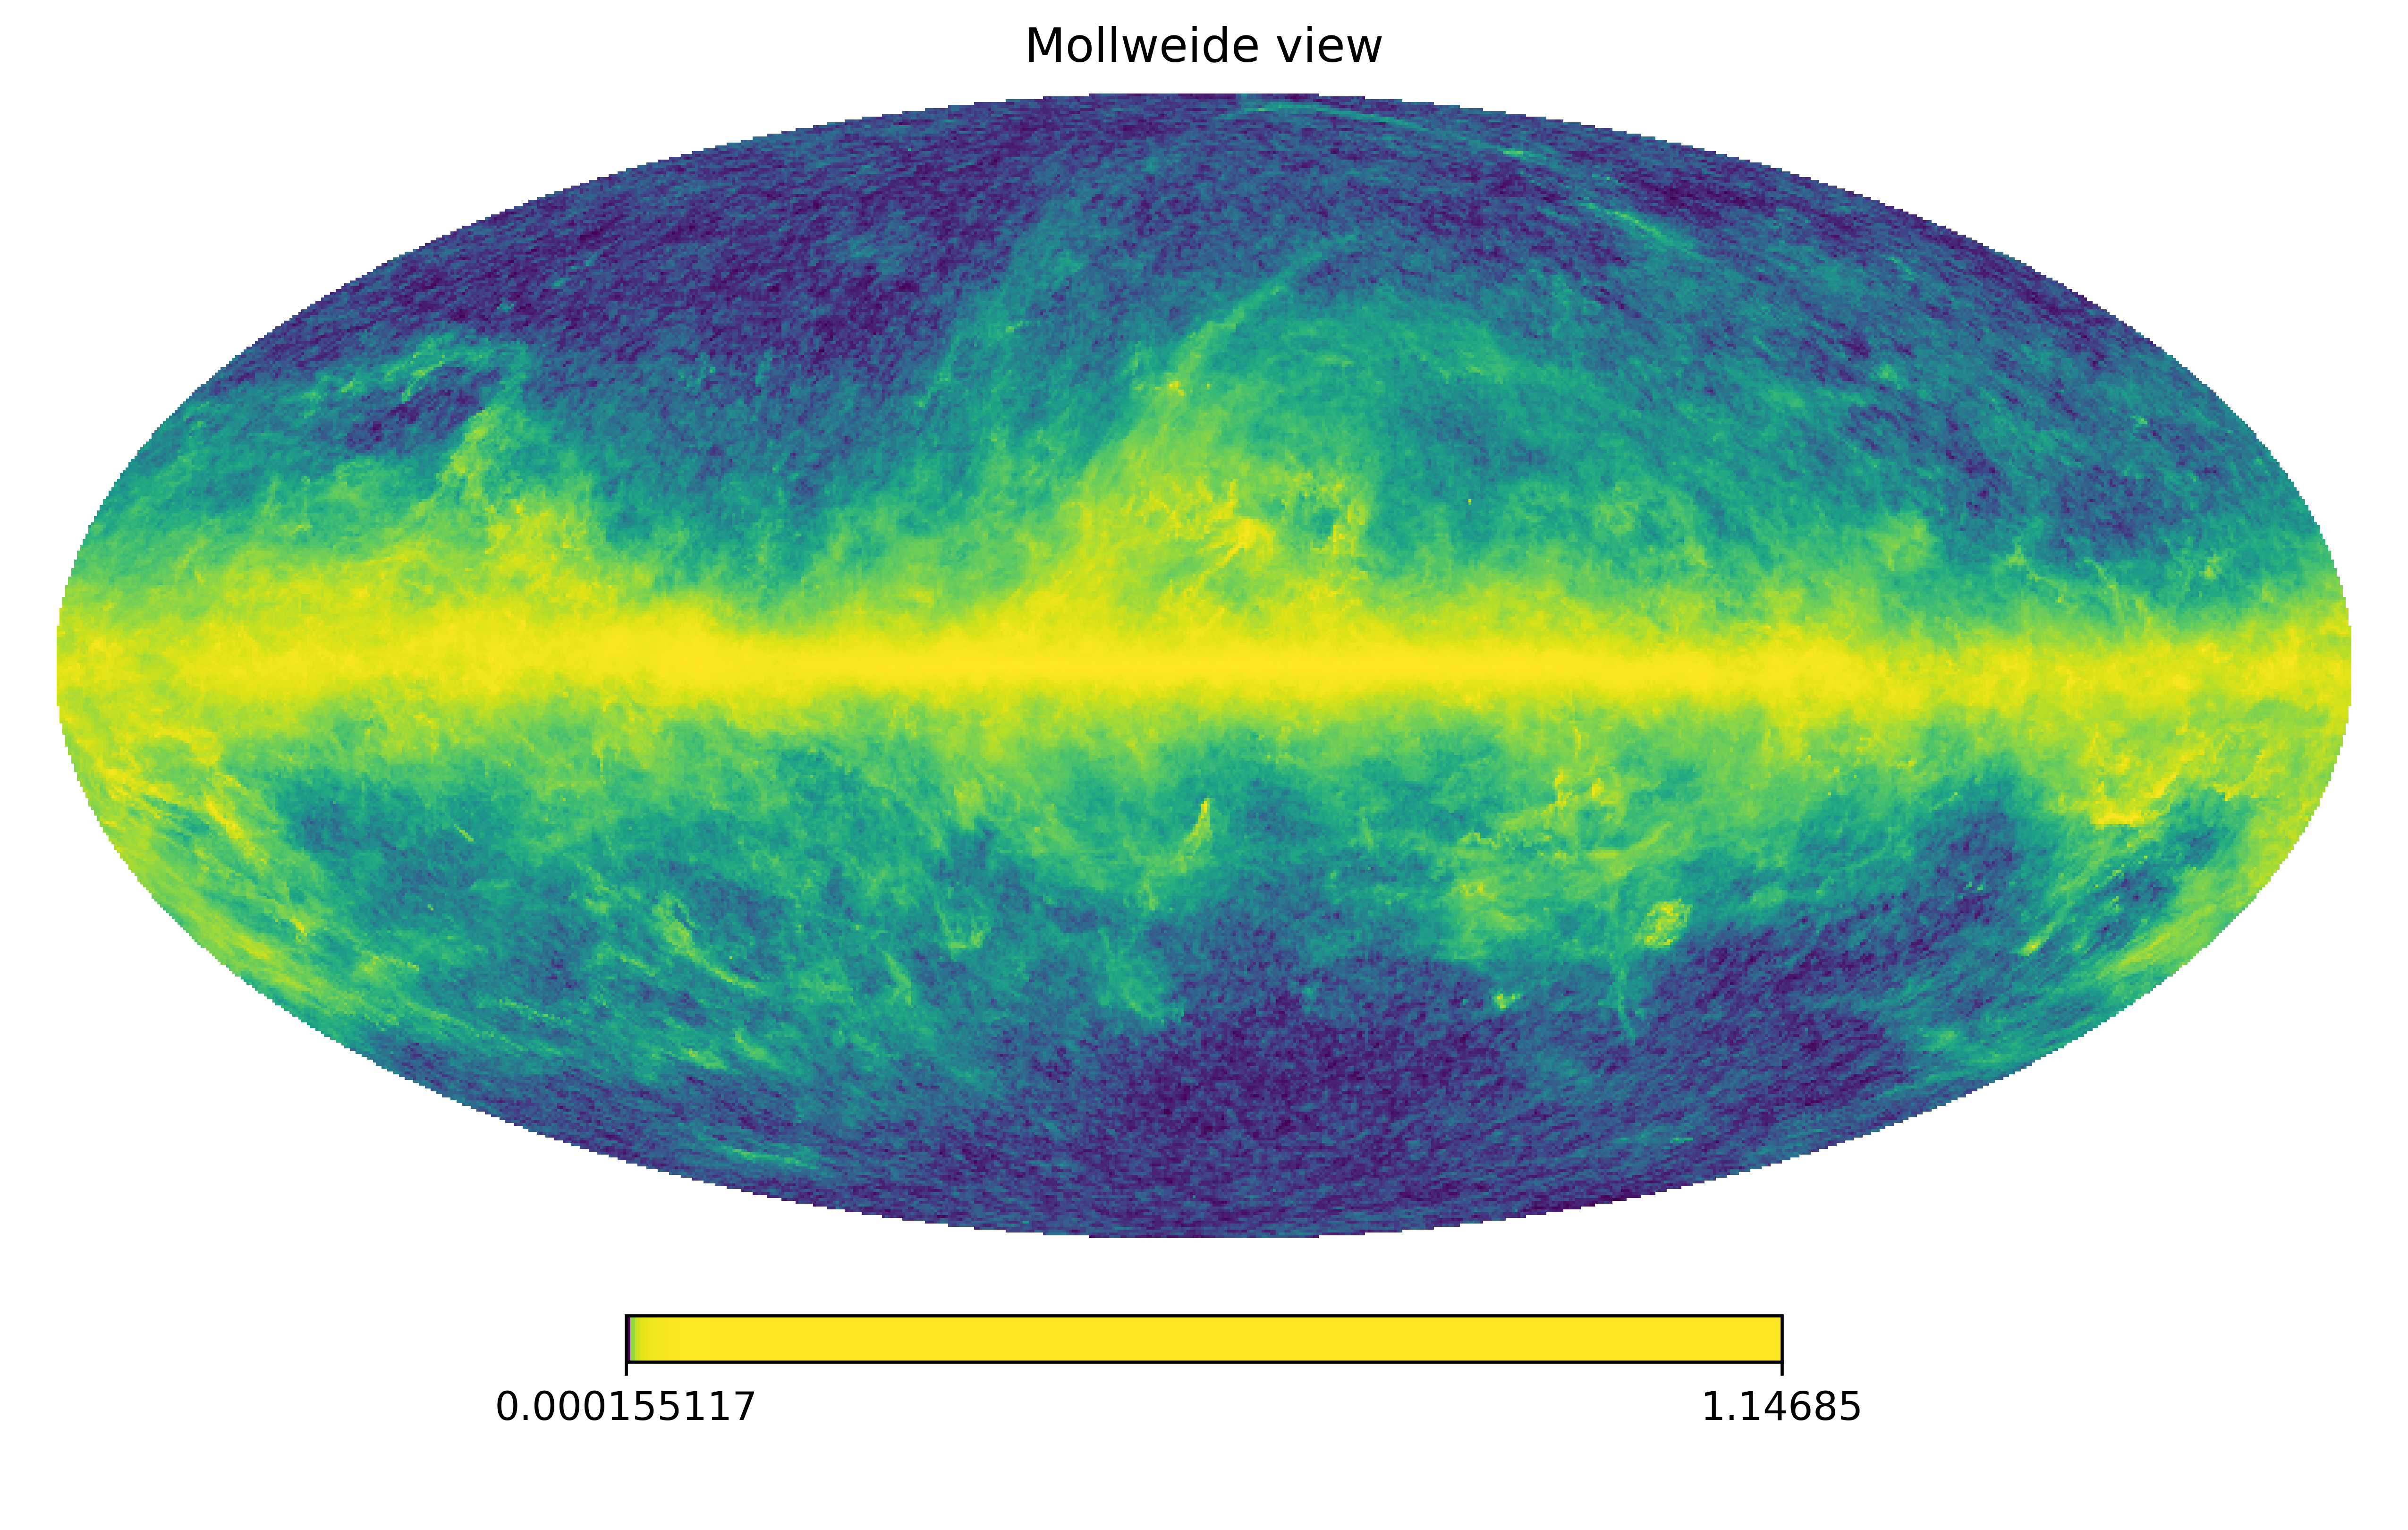
\includegraphics[scale=0.6]{figures/galactic_galaxy_map.png}
		\caption{Mollweide view of the\textit{ Sky Map} in \textbf{Galactic Coordinates}. The more yellow a point, the higher the temperature in said position. In order to enhance the features, the color scale has been normalized.}
		\label{sky_map_galactic}
		\end{figure}	
		
		The steps I took in order to get a \textit{mask} to juxtapose the Sky Map to the data from Plank/HFI are as follows:
		\begin{itemize}
			\item \textbf{Rotation}.\\
			The $353~\unit{GHz}$ map in the \textit{PLA} is saved in \textit{Galactic Coordinates}, while the pointing information in the timelines is recorded in \textit{Ecliptic Coordinates}, whose \textit{fundamental plane} is the Earth's Orbit's one (called \textit{Ecliptic plane}). 
			I decided that the best way to work with the data was to change the Sky Map from \textit{Galactic Coordinates} to \textit{Ecliptic Coordinates}.  \cite{coordinates_info}
			
			\item \textbf{Normalization}.\\
			As I was only interested in those sky patches where the Galaxy is too bright, but not it their absolute brightness, I have normalized the temperature in each pixel.
			Calling $x^{(old)}_i $ the values of the \textit{Sky Map} after the rotation but prior to the normalization and $x^{(new)}_i $ the normalized value:
			\[
				x^{(new)}_i = \frac { x^{(old)}_i - \min_{i} \{ x^{(old)} \}_i } { \max_{i}  \{ x^{(old)} \}_i } 
			\]
			where $i$ in the index that spans the whole collection.
			
			\item \textbf{Threshold}.\\
			I selected a \textit{threshold}, to convert the temperature map into a \textit{Boolean map}: every pixel whose value $x_i^{(new)}$ is greater than the threshold is set to $1$, and $0$ otherwise.
			The threshold I used was:
			\[
				threshold = 0.01
			\]
			I choose this value by trial and error.
		\end{itemize}
		In Fig. \ref{dust_mask} I show the \textbf{mask} I obtained using the procedure described.
		
		\begin{figure}[t]
		\centering
		\includegraphics[scale=0.6]{figures/Elliptic_galaxy_mask.png}
		\caption{Mollweide view in \textit{Ecliptic Coordinates} of the mask used on the Plank/HFI data. The yellow points are discarded in my analysis.}
		\label{dust_mask}
		\end{figure}
		
		I used the mask to remove samples from the timestreams recorded by \textit{HFI}'s bolometers.
		In Fig. \ref{mask_data} I show an example of the results obtained.
		
		\begin{figure}[h!]
			\centering
			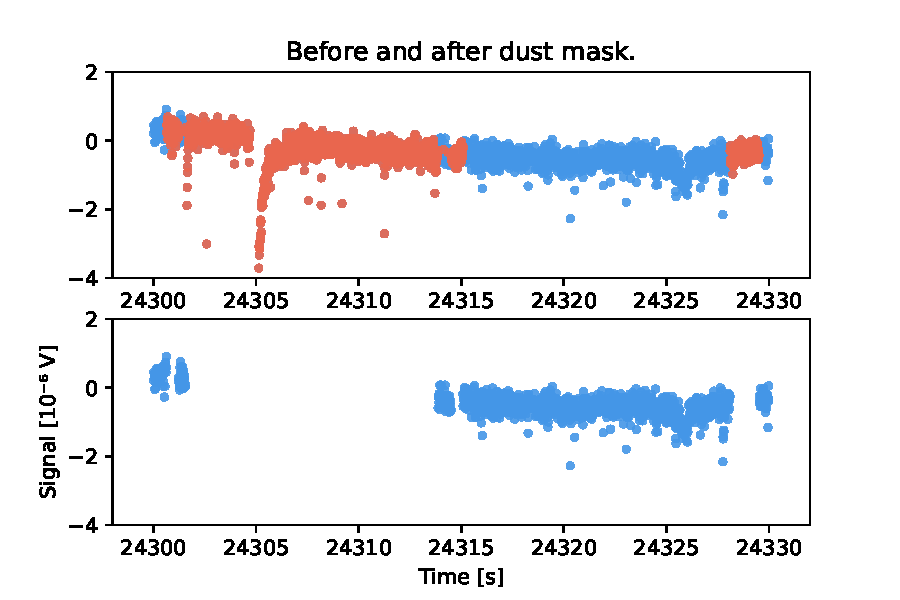
\includegraphics[scale=0.65]{figures/no_gal_signal.pdf}
			\caption{$30$ seconds for the detector \texttt{100-1a} for the day $93$, before and after the mask cleaning. Some points may be taken out even if, visually, it seems that no Galactic signal is present: that is mostly due to noise.}
			\label{mask_data}
		\end{figure}

%
%
%
		\subsection{CMB Dipole} \label{sec_dipole}
		
			The motion of the Sun with respect to the rest frame of the CMB generates a Doppler effect: this results in the presence of a \textbf{dipole} in the CMB data, whose peak-to-peak amplitude is approximately $3~\unit{mK}$.\cite{CMB_dipole}
				Similarly to what I did with the Galactic Signal in Section \ref{Milky_way}, I removed the dipole from the data.			
			
				Given the speed of the solar system with respect to the rest frame of the CMB, $|\vec v_{sun} |= 369 \pm 2.5 ~\unit{\sfrac {Km}{s}}$ \cite{CMB_dipole}, and the base temperature of the cosmic background, $T_0 = 2.72548 \pm 0.00057 ~\unit{K}$ \cite{CMB_temperature}, the temperature of the dipole in a given direction of the sky, $\vec x = (\theta, \varphi)$, is:
				\[
					T(\vec x) = T_0 \cdot \left( \frac { 1 }  {\gamma \cdot \left(  1 - \vec x \cdot \vec \beta \right) }-1 \right) 
				\]
				where $\vec \beta = \sfrac { \vec v_{sun}}{c}$ and $\gamma = \left( 1 - \beta^2 \right) ^{-\sfrac 1 2 } $. 				
				
				Since the \textit{HFI} acquisition electronics saved even values in the timestream with the negative sign, I computed consecutive averages of the positions, hence $\vec x_{\Delta V_i } = \left( \vec x _{i+1} - \vec x _i \right) \cdot \sfrac 1 2 $. In this way, I halved the amount of data to process.				
				
			Once obtained all of the values for the dipole corresponding to a certain batch of data (Fig. \ref{dipole_example}), I subtracted it to the values of the voltages themselves. In order to match the units of measure between the two, a simple regression was executed as follows.
			\begin{figure}
			\centering
			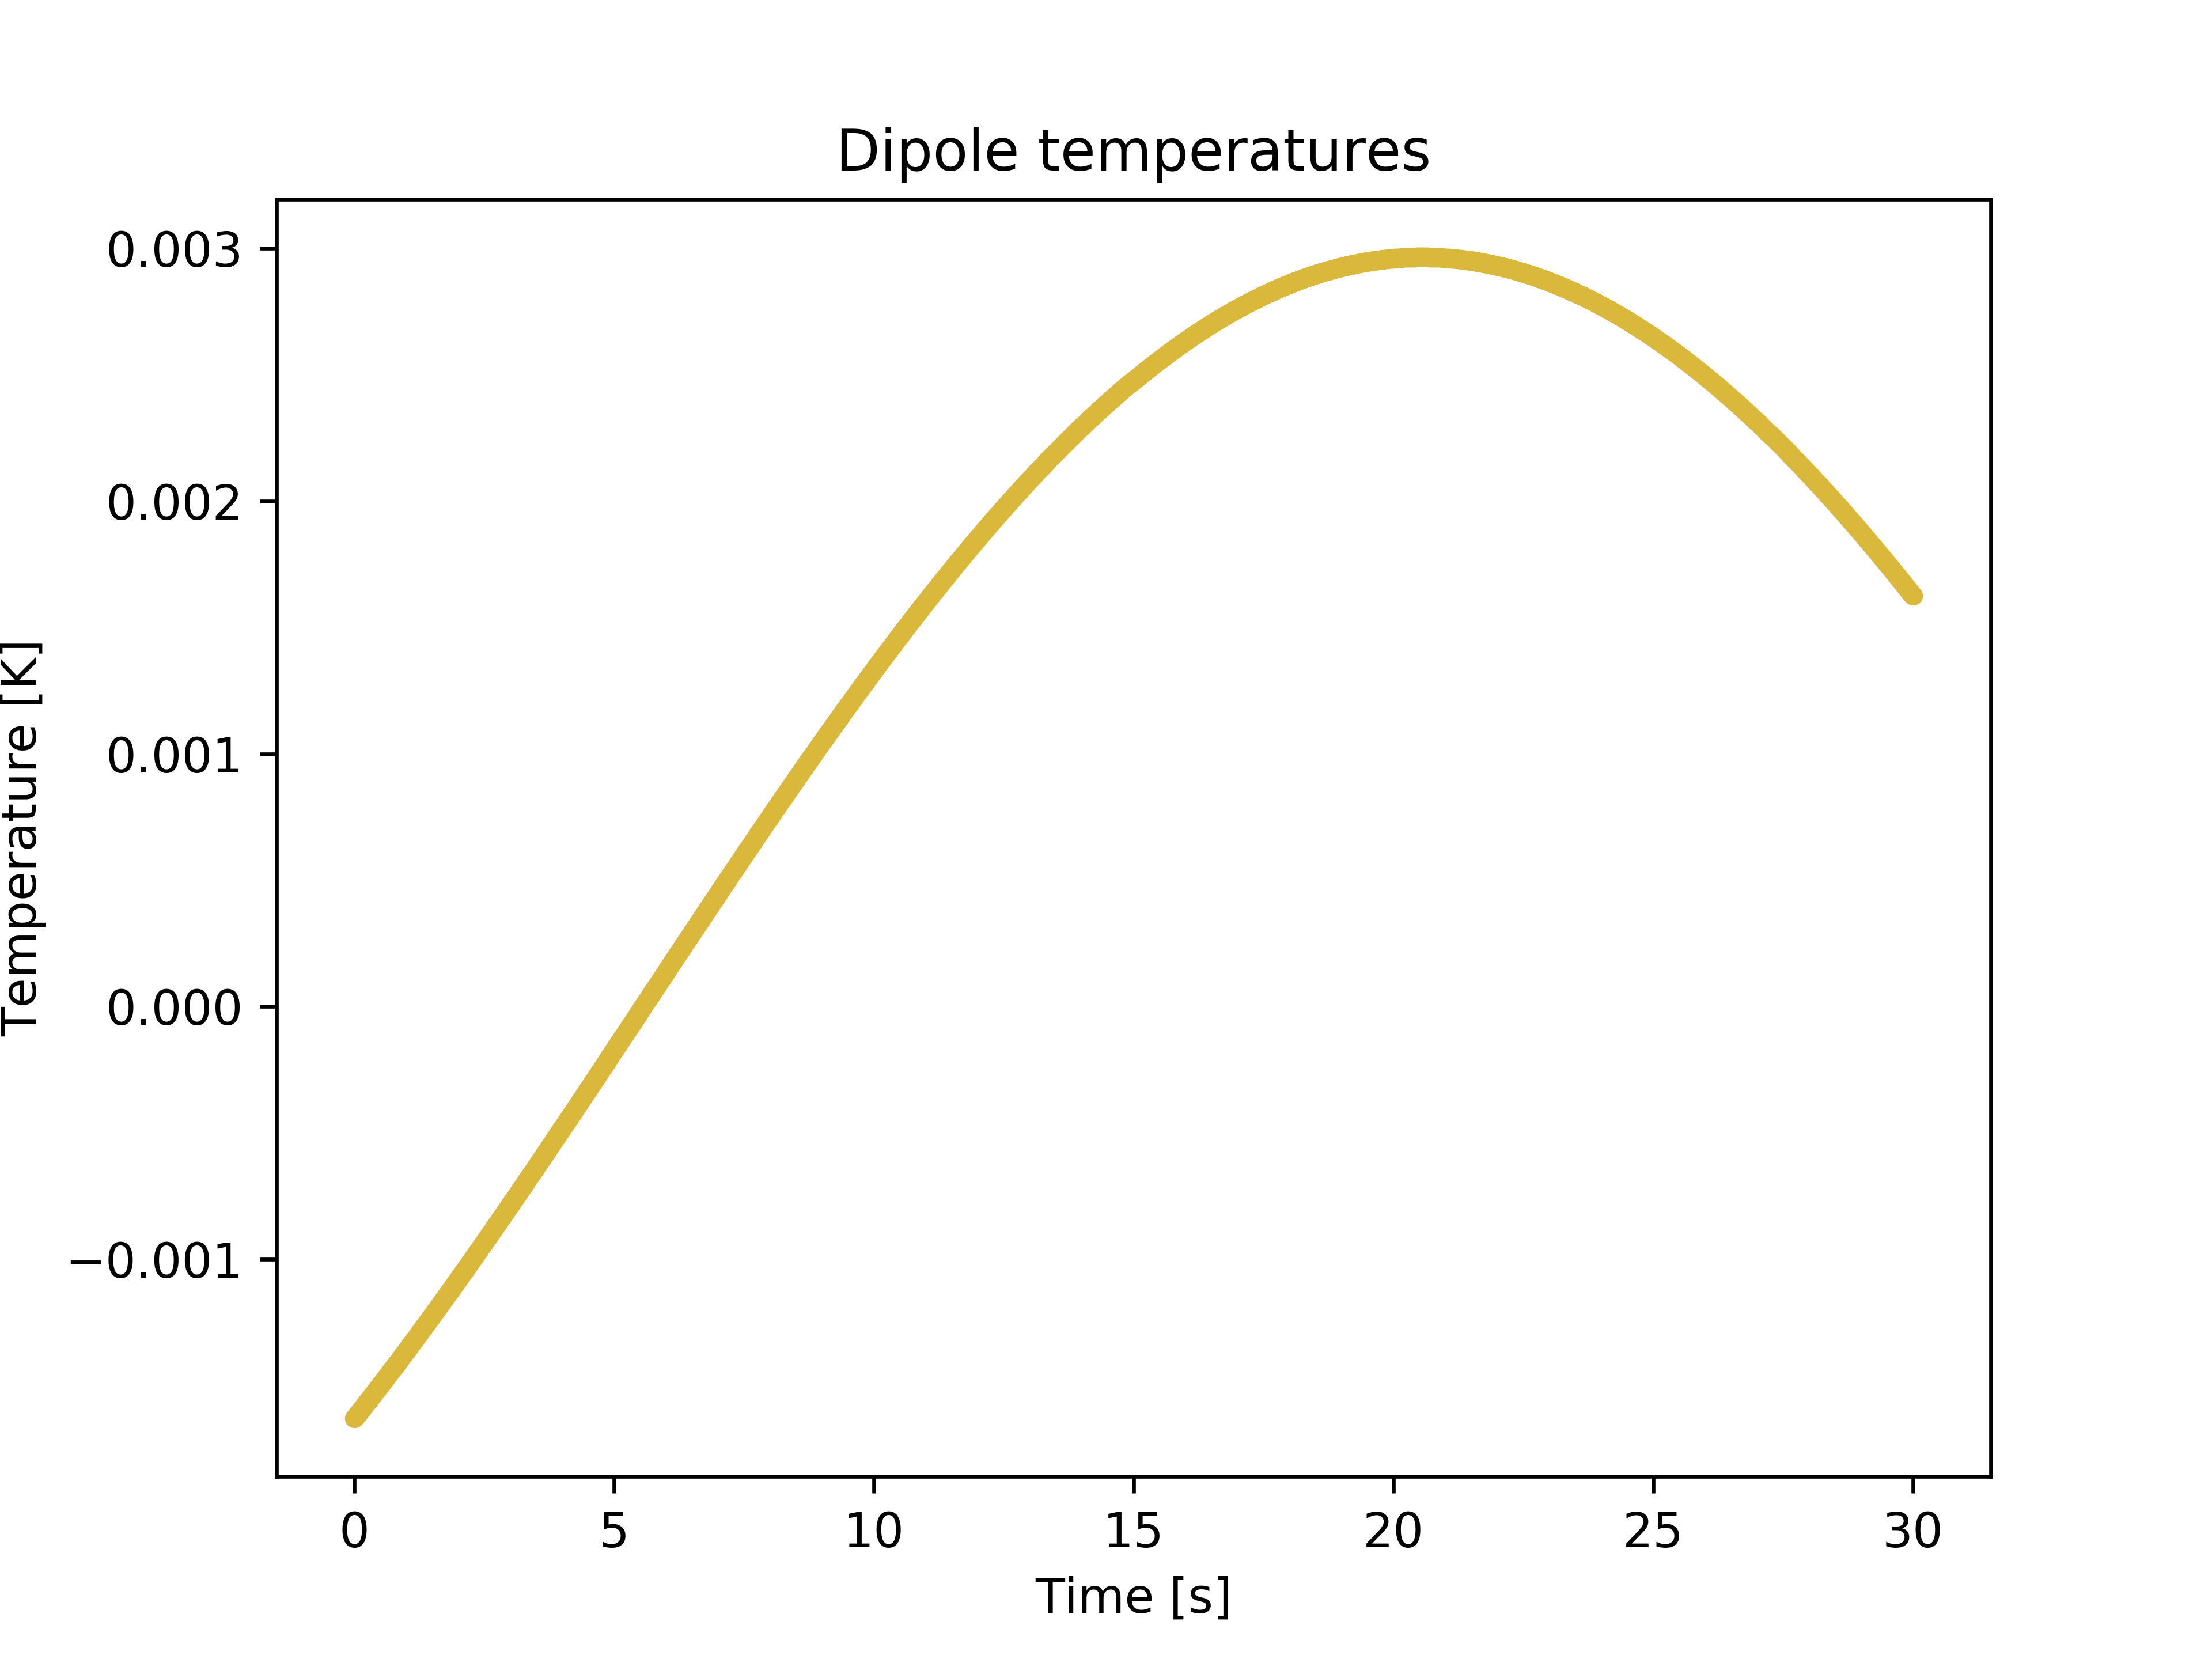
\includegraphics[scale=0.65]{figures/dipole_example.png}
			\caption{An example of the dipole temperatures as computed for 30 seconds, for the detector \texttt{100-1a} for the day $93$. On the $y$ axis is the intensity of the dipole: one can see that its maximum value is approximately $3~\unit{mK}$}
			\label{dipole_example}
		\end{figure}		
			Firstly, I scaled both the dipole temperatures and the bolometer voltages to their respective medians, as the correlation is:
			\[
				\Delta V(\vec x ) - \Delta V_0 = G \cdot ( T (\vec x ) - T_0 ) 
			\] 
			where $\Delta V_0$ and $T_0$ are the median of the satellite voltages and the dipole temperatures respectively. I used a \textit{least square regression} to figure out $G$, then subtracted the dipole:
			\[
				\Delta V_{clean } (\vec x ) = (\Delta V (\vec x ) - \Delta V_0 )  - G \cdot ( T (\vec x ) - T_0 ) 
			\]
			where $\Delta V_{clean } (\vec x )$ is the new data, clean of the CMB dipole.			
			
			Fig. \ref{before_after_dipole} shows an example of some data where the dipole has been removed: the oscillatory behavior, typical of the CMB dipole, is no longer present.			
					
				Some dipole residual is still present in the data, due to the Doppler effect caused by the velocity of the Planck satellite with respect to the Sun rest frame. While it is possible to evaluate it\footnote{In order to compute the Doppler effect caused by the space probe's motion, one should have to evaluate the exact speed (module and direction) for each position, and then add it to the calculation of the Dipole effect.}, the removal of the dipole caused by the motion of the \textit{Solar System} is good enough for the purposes of this thesis. 
			 
			\begin{figure}
			\centering
			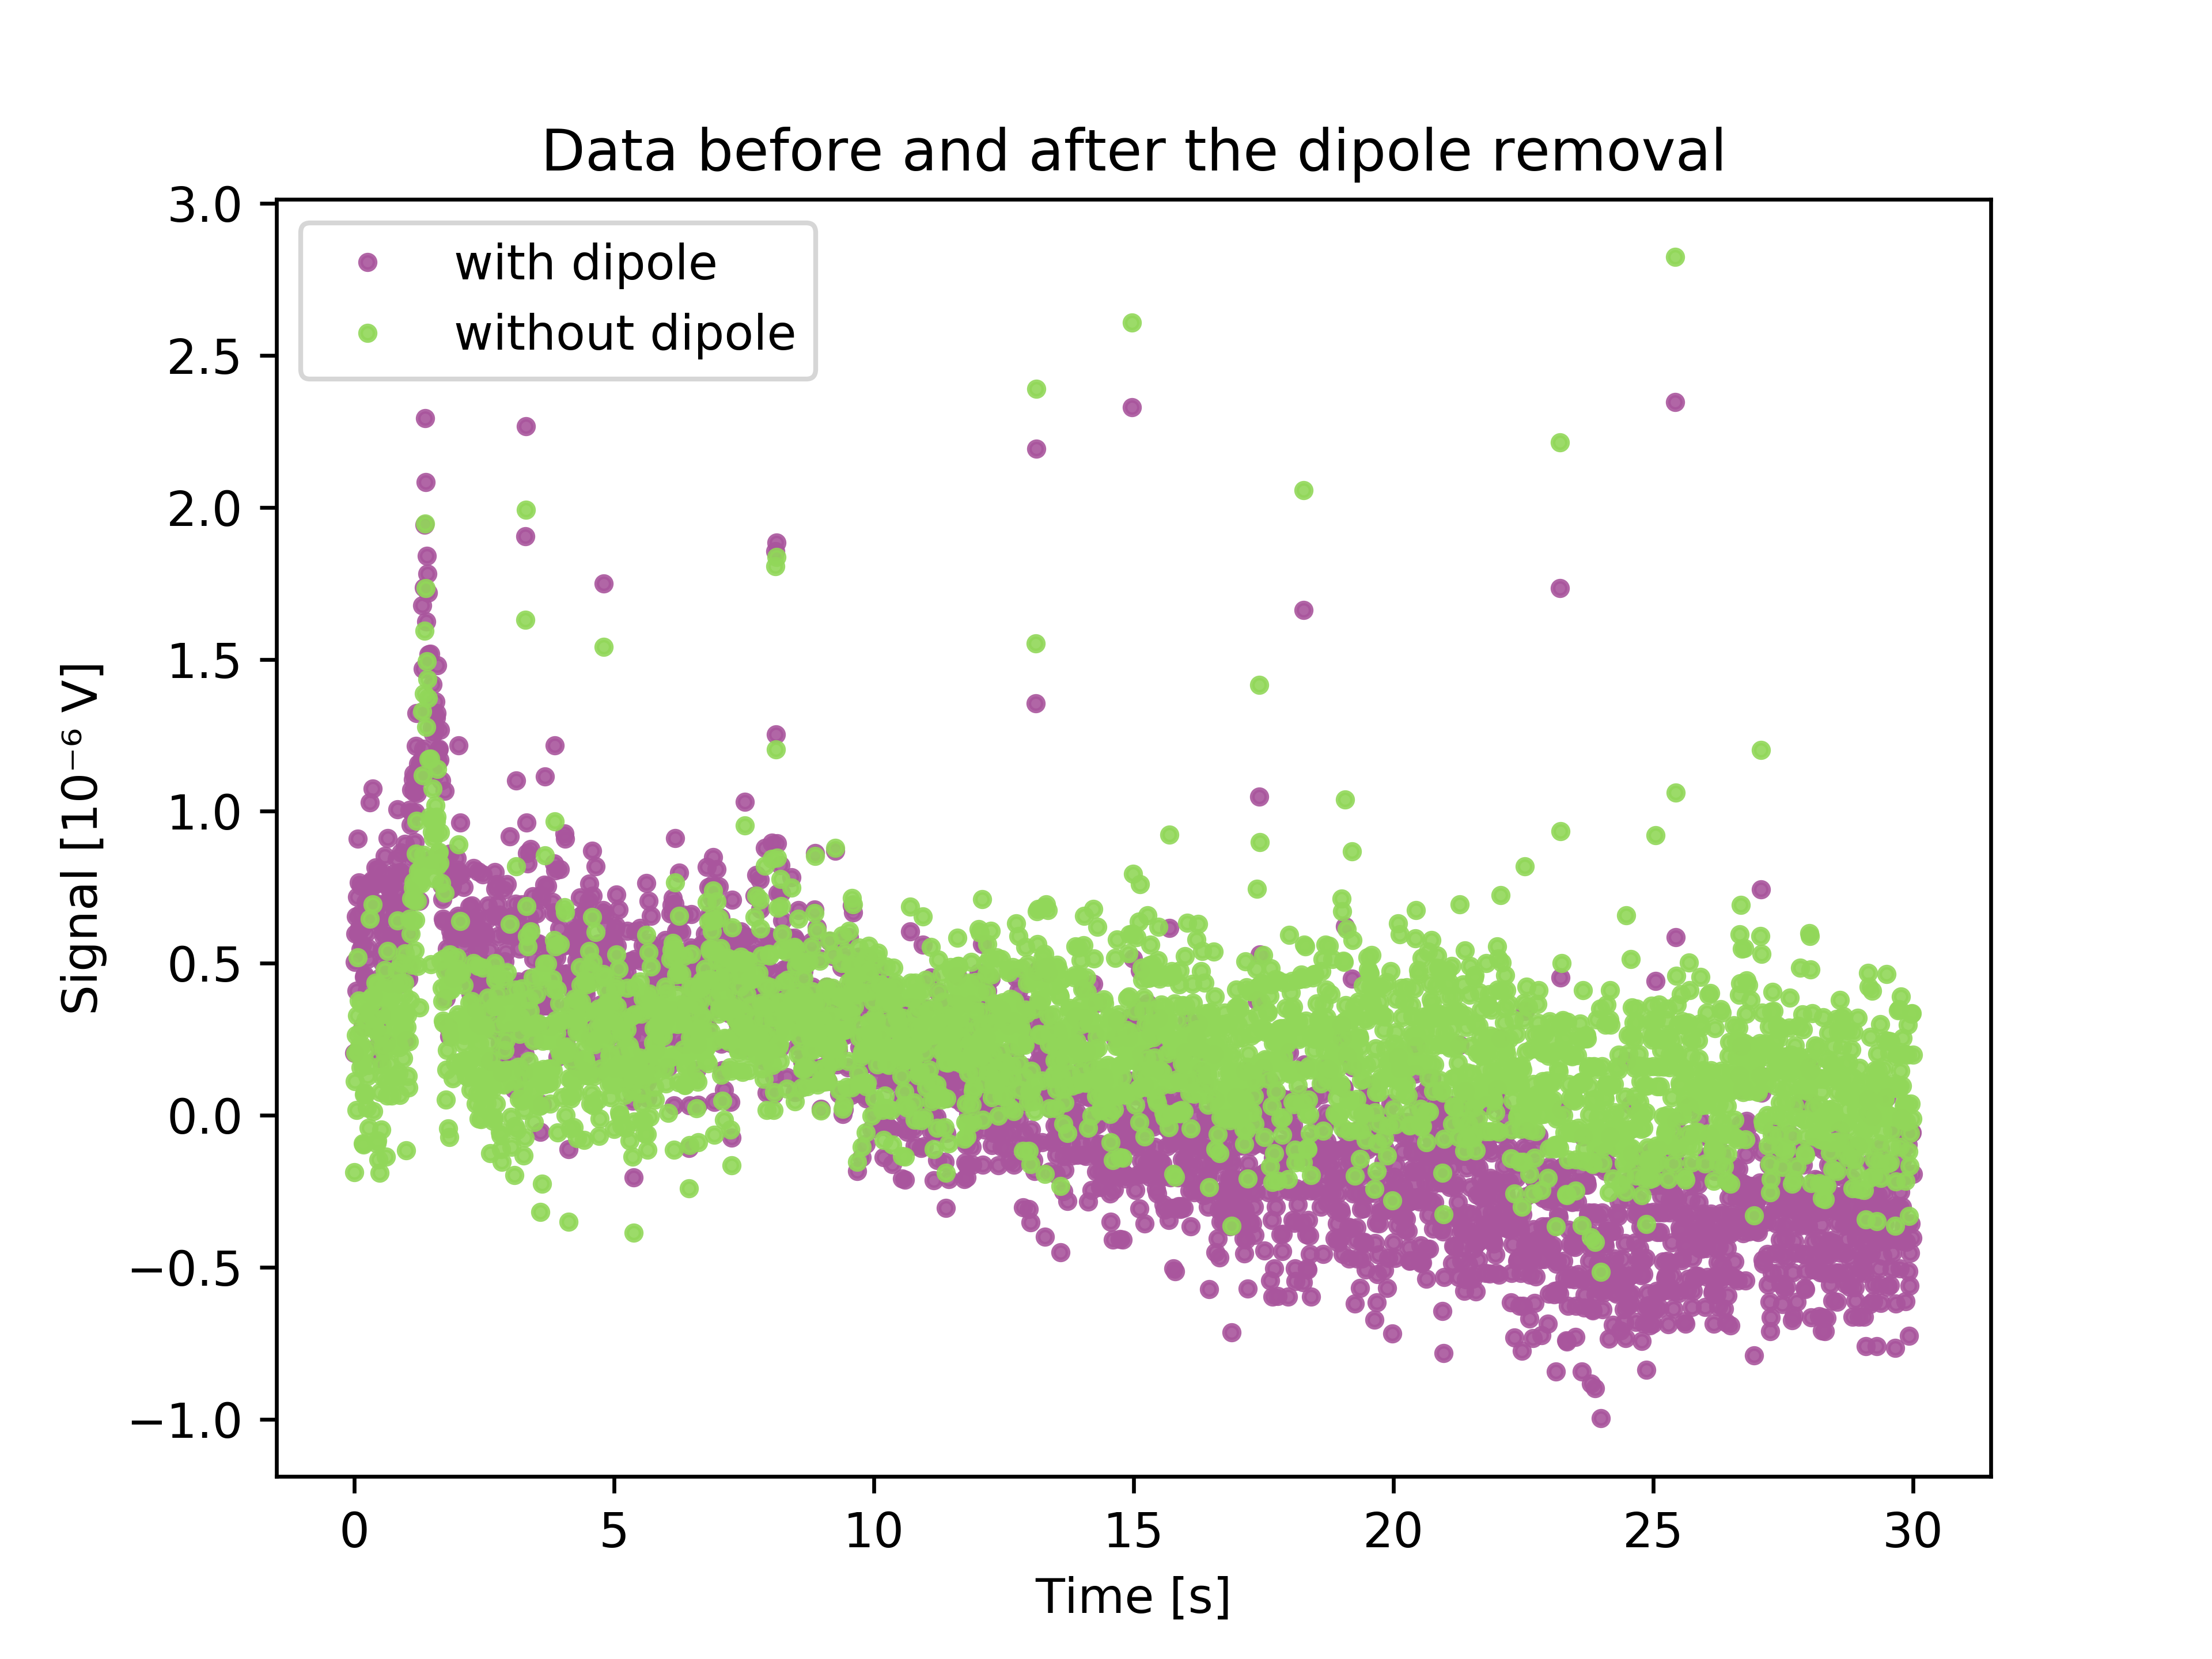
\includegraphics[scale=0.65]{figures/before_after_dipole.png}
			\caption{An example of the effect of the dipole removal on some data, from the bolometer \texttt{100-1a} for the day $94$. It is easy to see that the ``cleaned data" has a way less periodic oscillation.}
			\label{before_after_dipole}
		\end{figure}			
				
		\section{Data Classification}\label{data_classification}
		
			Once I obtained some batches of data cleaned as described above, in Section \ref{data_preparation}, I classified data by hand using the following approach.
						
			I took some randomly small chunks from a single day of recordings and, using a computer program, labeled them either as \textit{glitches} or \textit{non-glitches}.
			I only considered batches of unflagged data (see Section \ref{Milky_way}).			 
			
				I created a computer program that randomly selects a starting point from the whole day of recording, take the next 100 samples in the timestrem, and display on the screen. Then it asks the user if the data in the image contains a \textit{glitch} or not, saving the batch to a specific folder (either for \textit{glitch} or \textit{non-glitch}).
				In those cases where it is not clear how to classify the batch
				\footnote{With this, it means that the timeseries taken had values that were not easily distinguishable without knowing the data outside the initial and final points plotted. While it would have been possible to plot a few points outside of it, it was thought more effective to just discard uncertain cases and move on with the next.}
				, the program neglects it and selects a new starting position. 
				\begin{figure}[h]
   					\centering
				  \begin{subfigure}{0.6\textwidth}
				        \centering
				        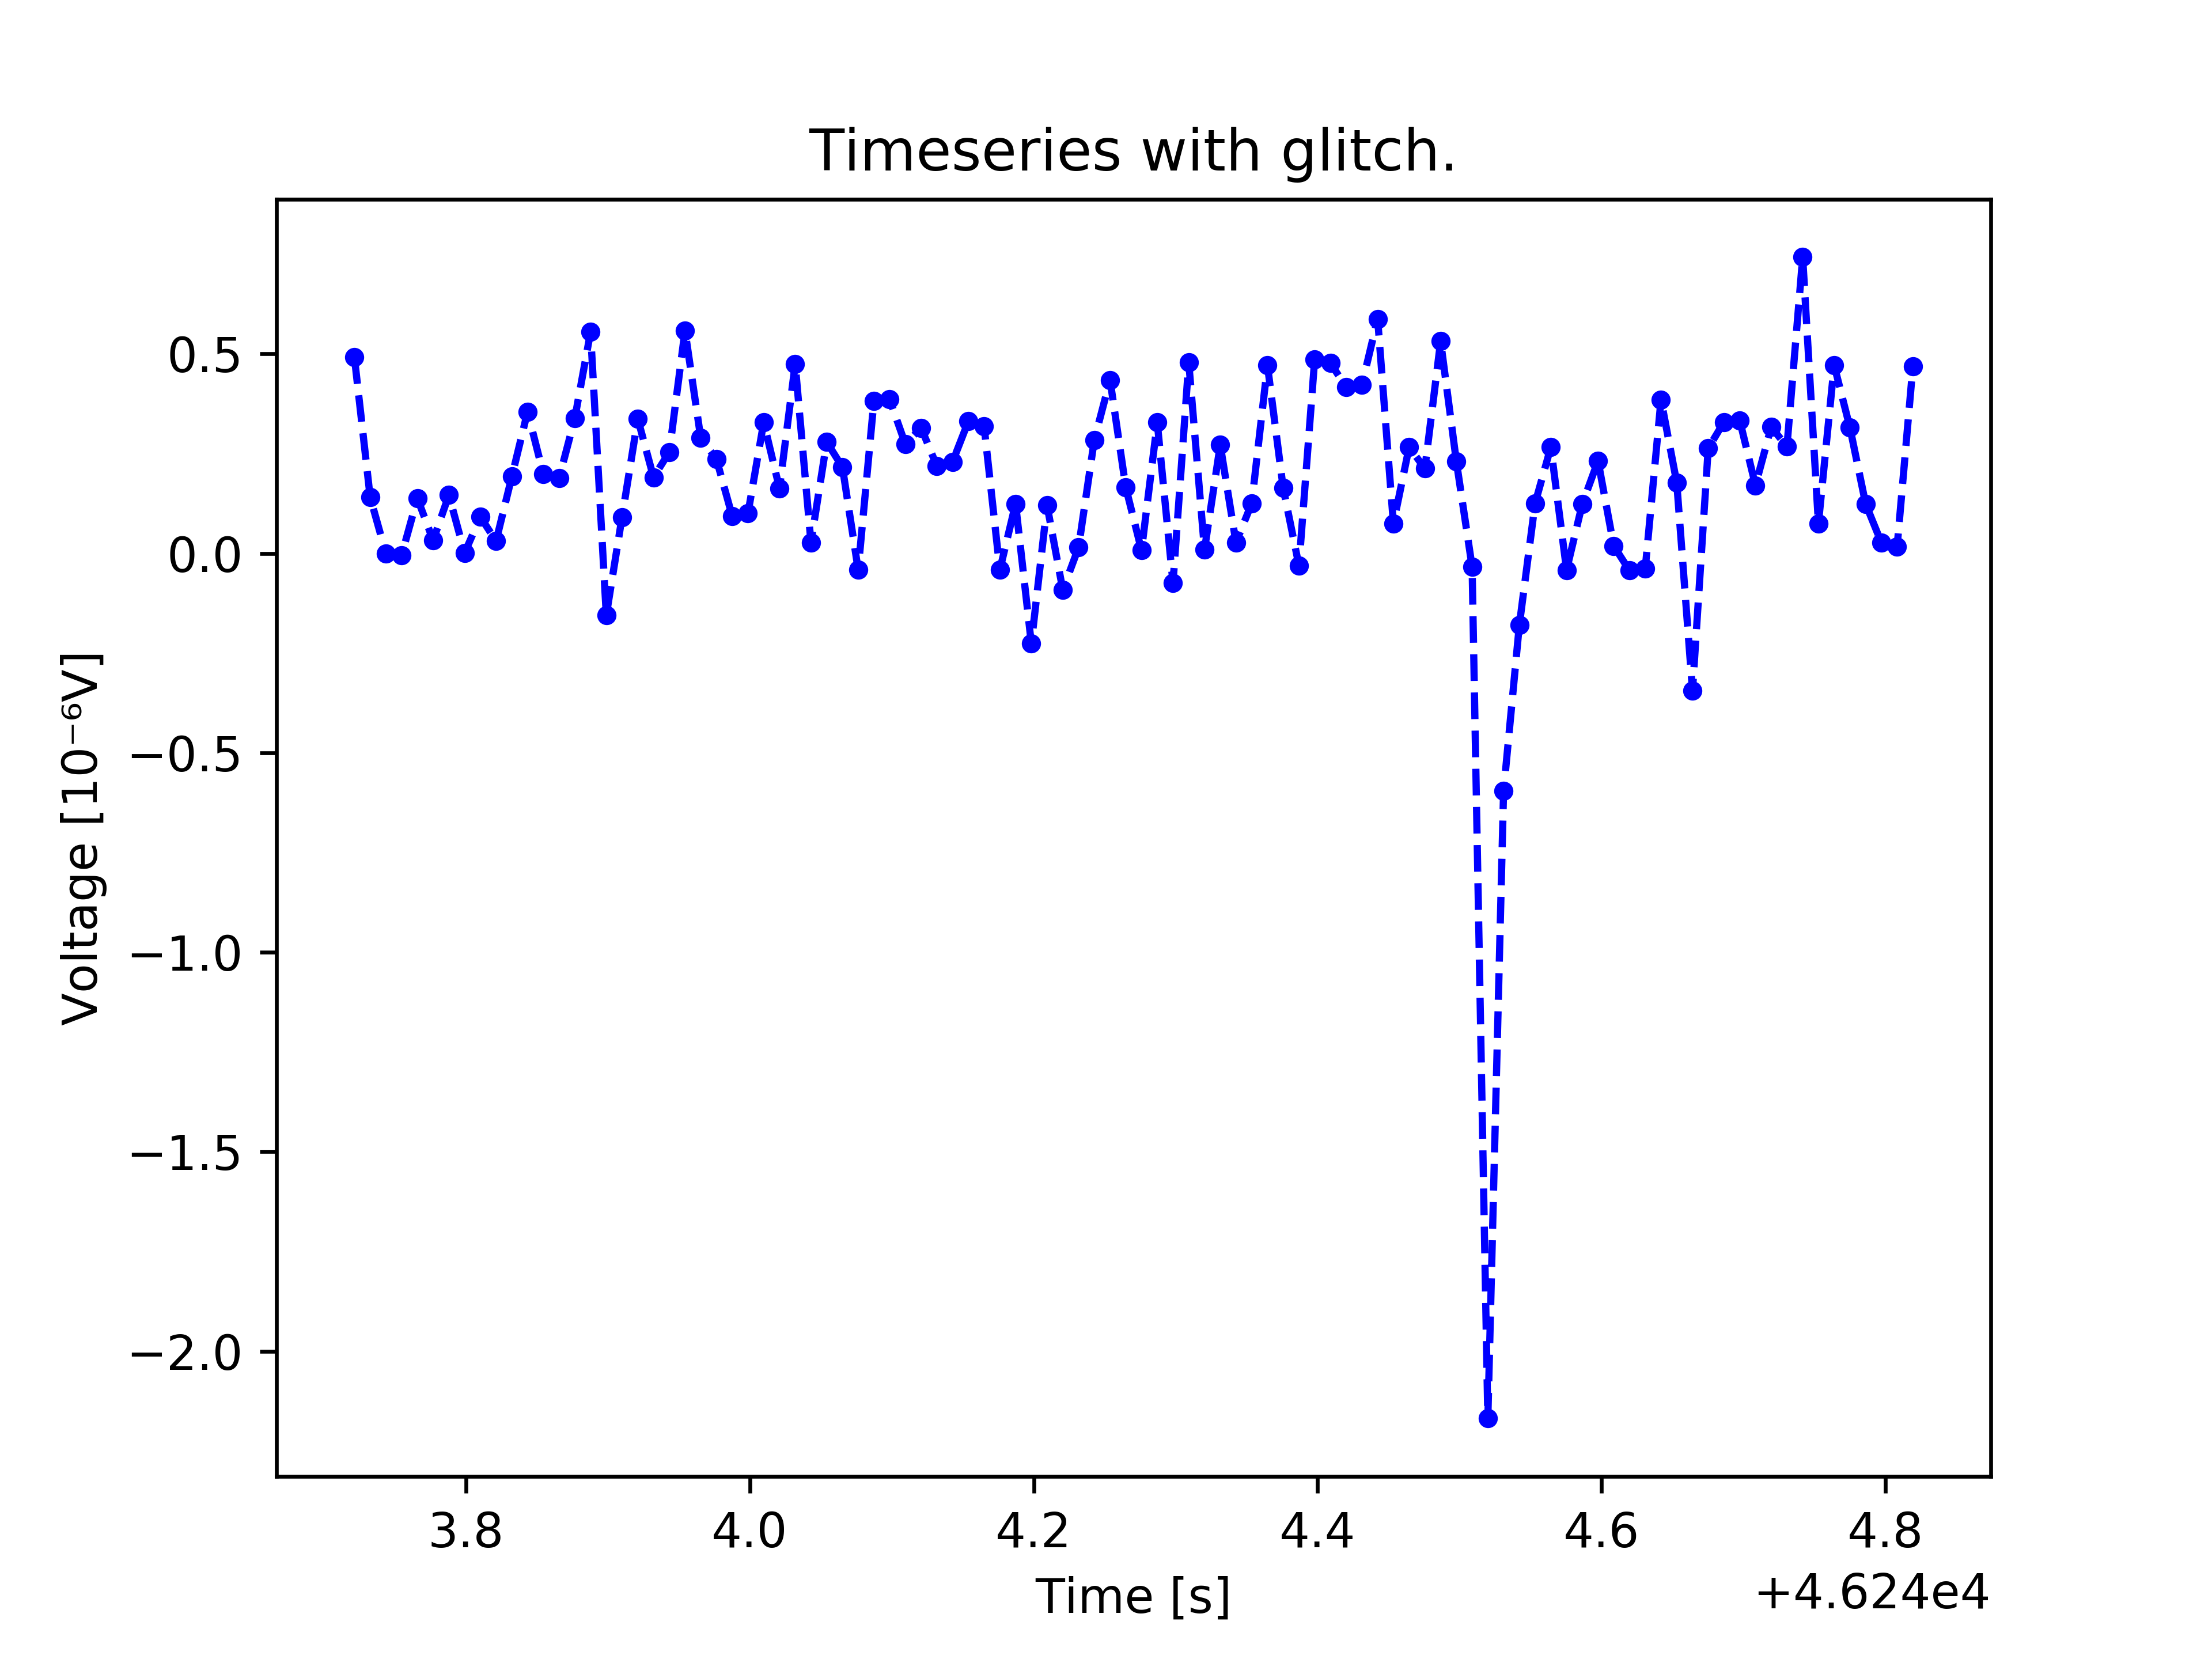
\includegraphics[scale=0.5]{figures/glitch.png}
				        \caption{}
			    \end{subfigure}%
			    \begin{subfigure}{0.6\textwidth}
					\centering
			        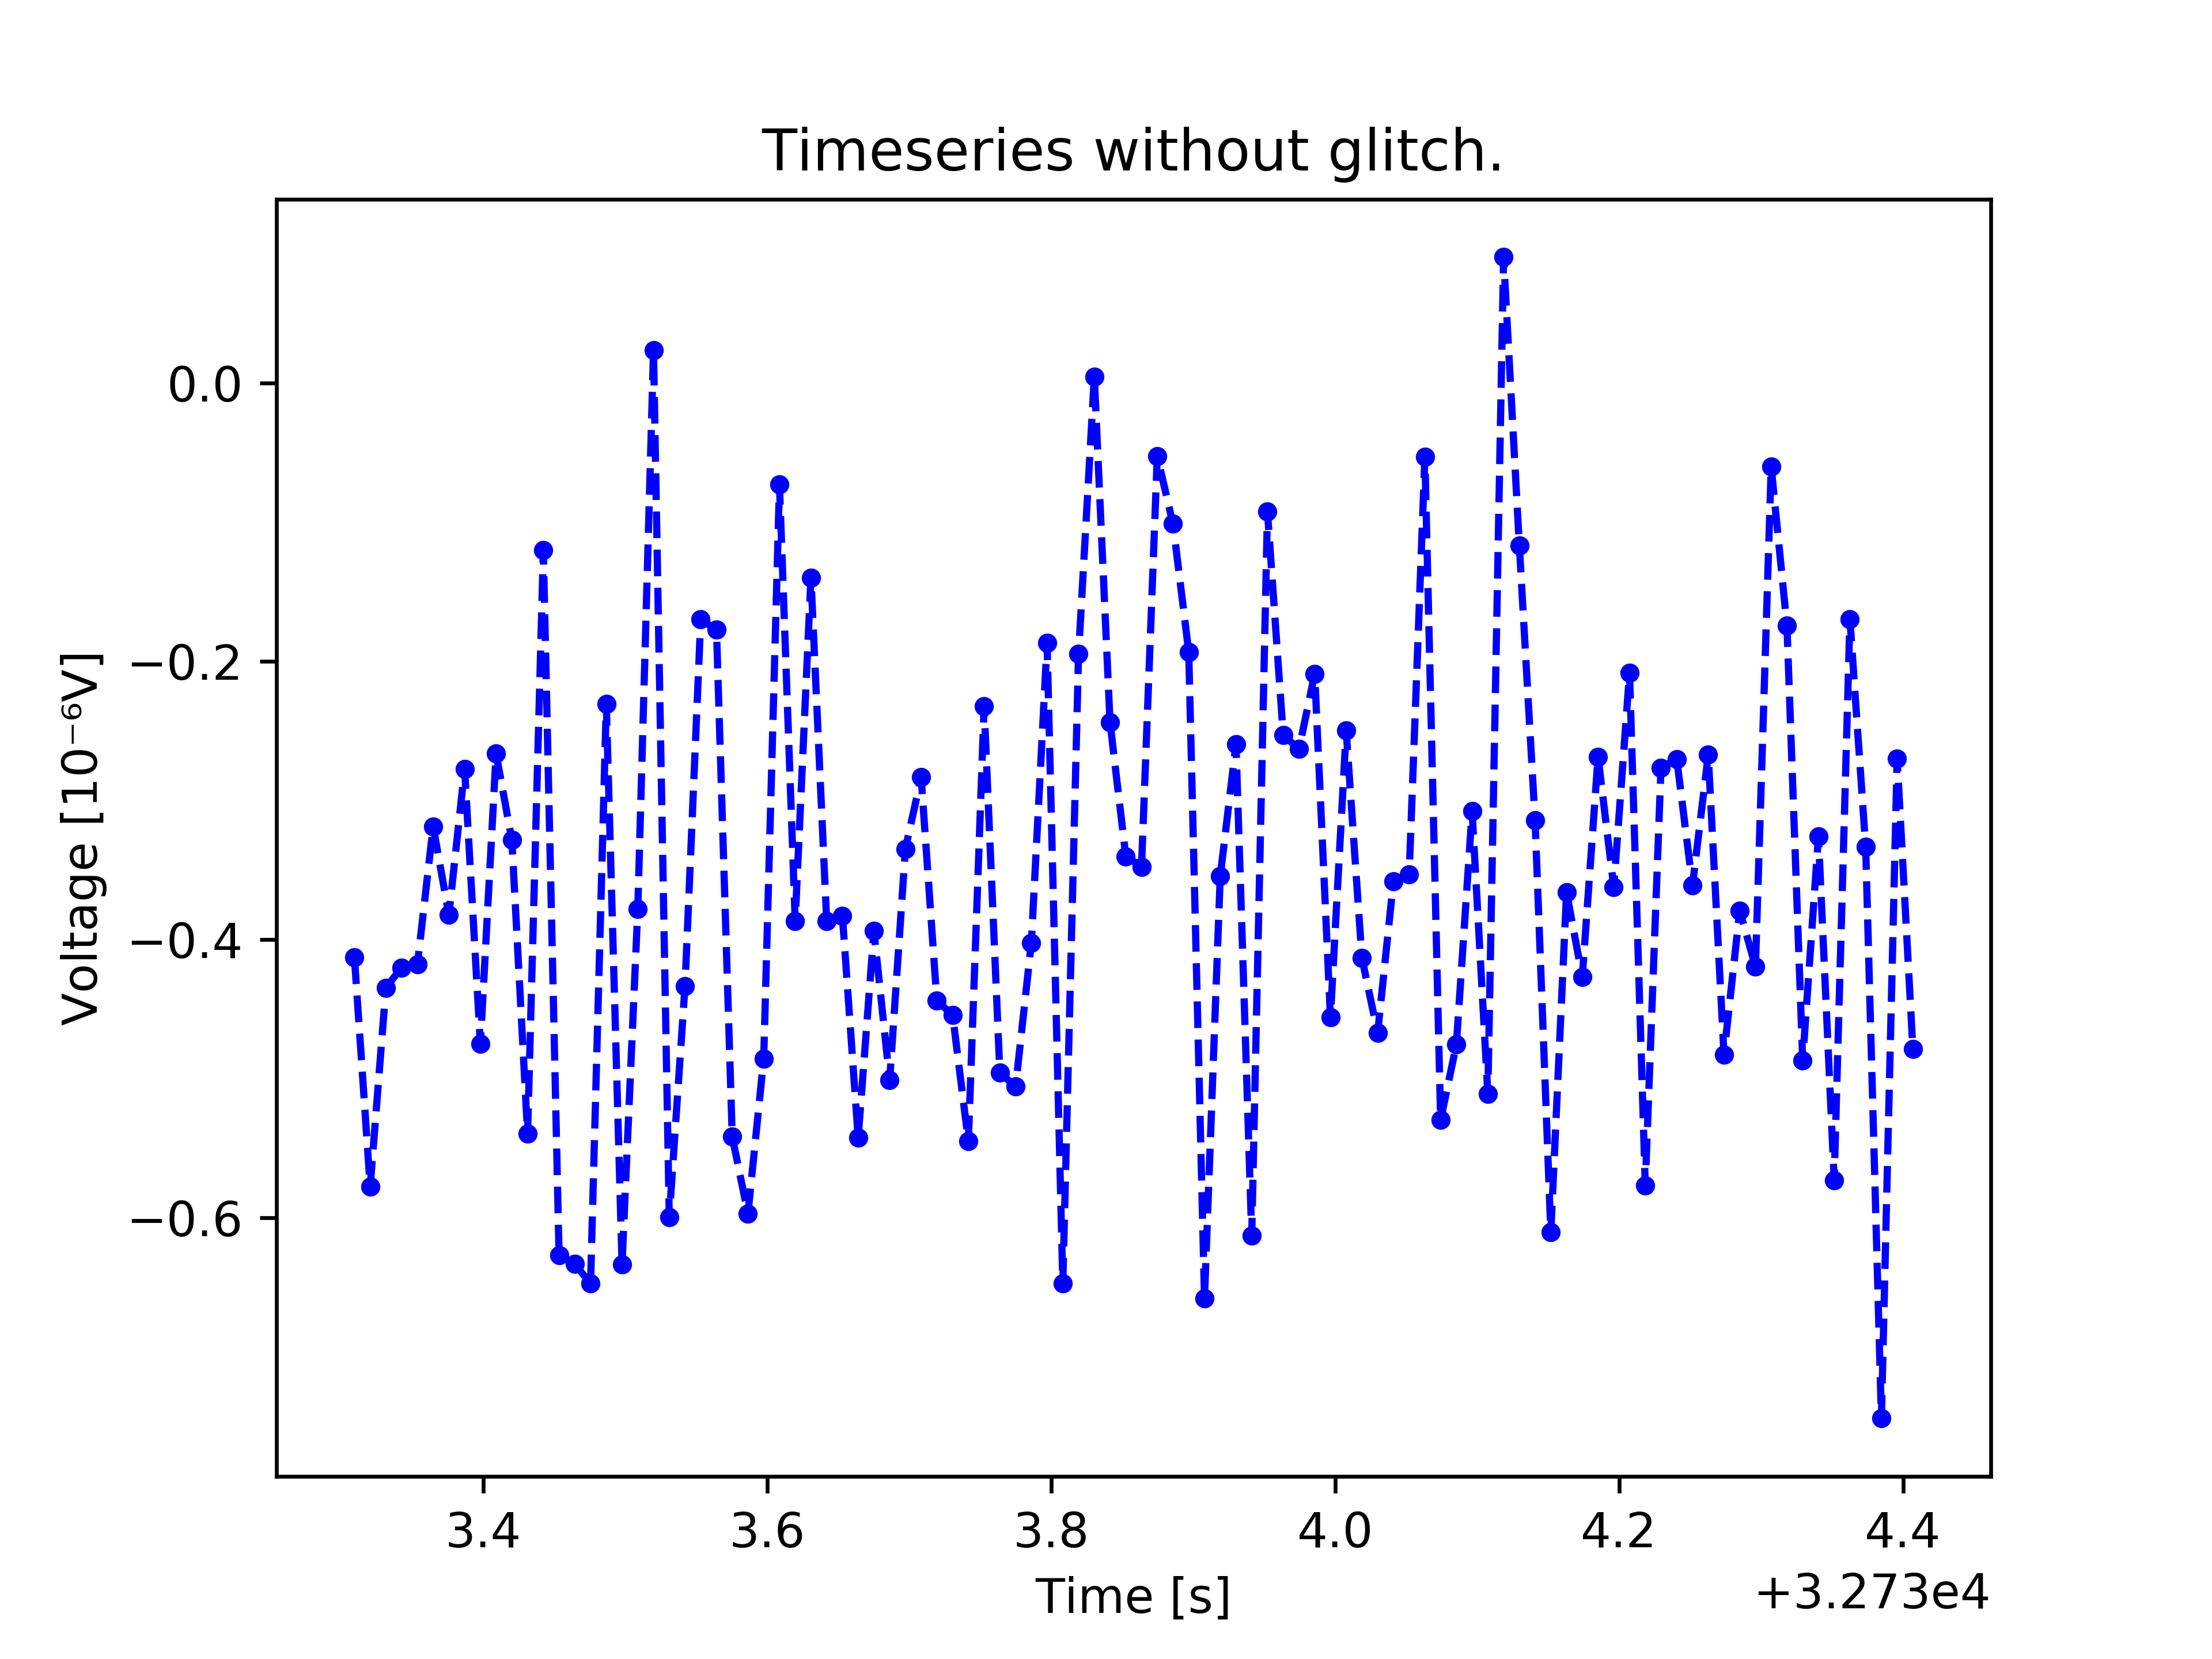
\includegraphics[scale=0.5]{figures/no_glitch.png}
					\caption{}
			    \end{subfigure}
			    \caption{Two examples of timeseries for the classification used. On the left (a), I show a glitch: a big spike compared to noise. On the right (b), a timeseries without any glitches.}
			    \label{timeseries_plot}
			\end{figure}			
				
				Fig. \ref{timeseries_plot} shows two plots, one classified as \textit{glitch} and one as \textit{not glitch}. As one can see, the glitch can bee easily spotted as a spike above the normal ``noise" of the detector. 
				Fig. \ref{unclassifiable_plot} shows an example of a case where there is not certainty, hence it is not taken into consideration. While in many of these cases it could be disputed about the presence of a glitch or not, I preferred to use as training data only those cases where I was certain about the classification.
				
				\begin{figure}[h!]
					\centering
					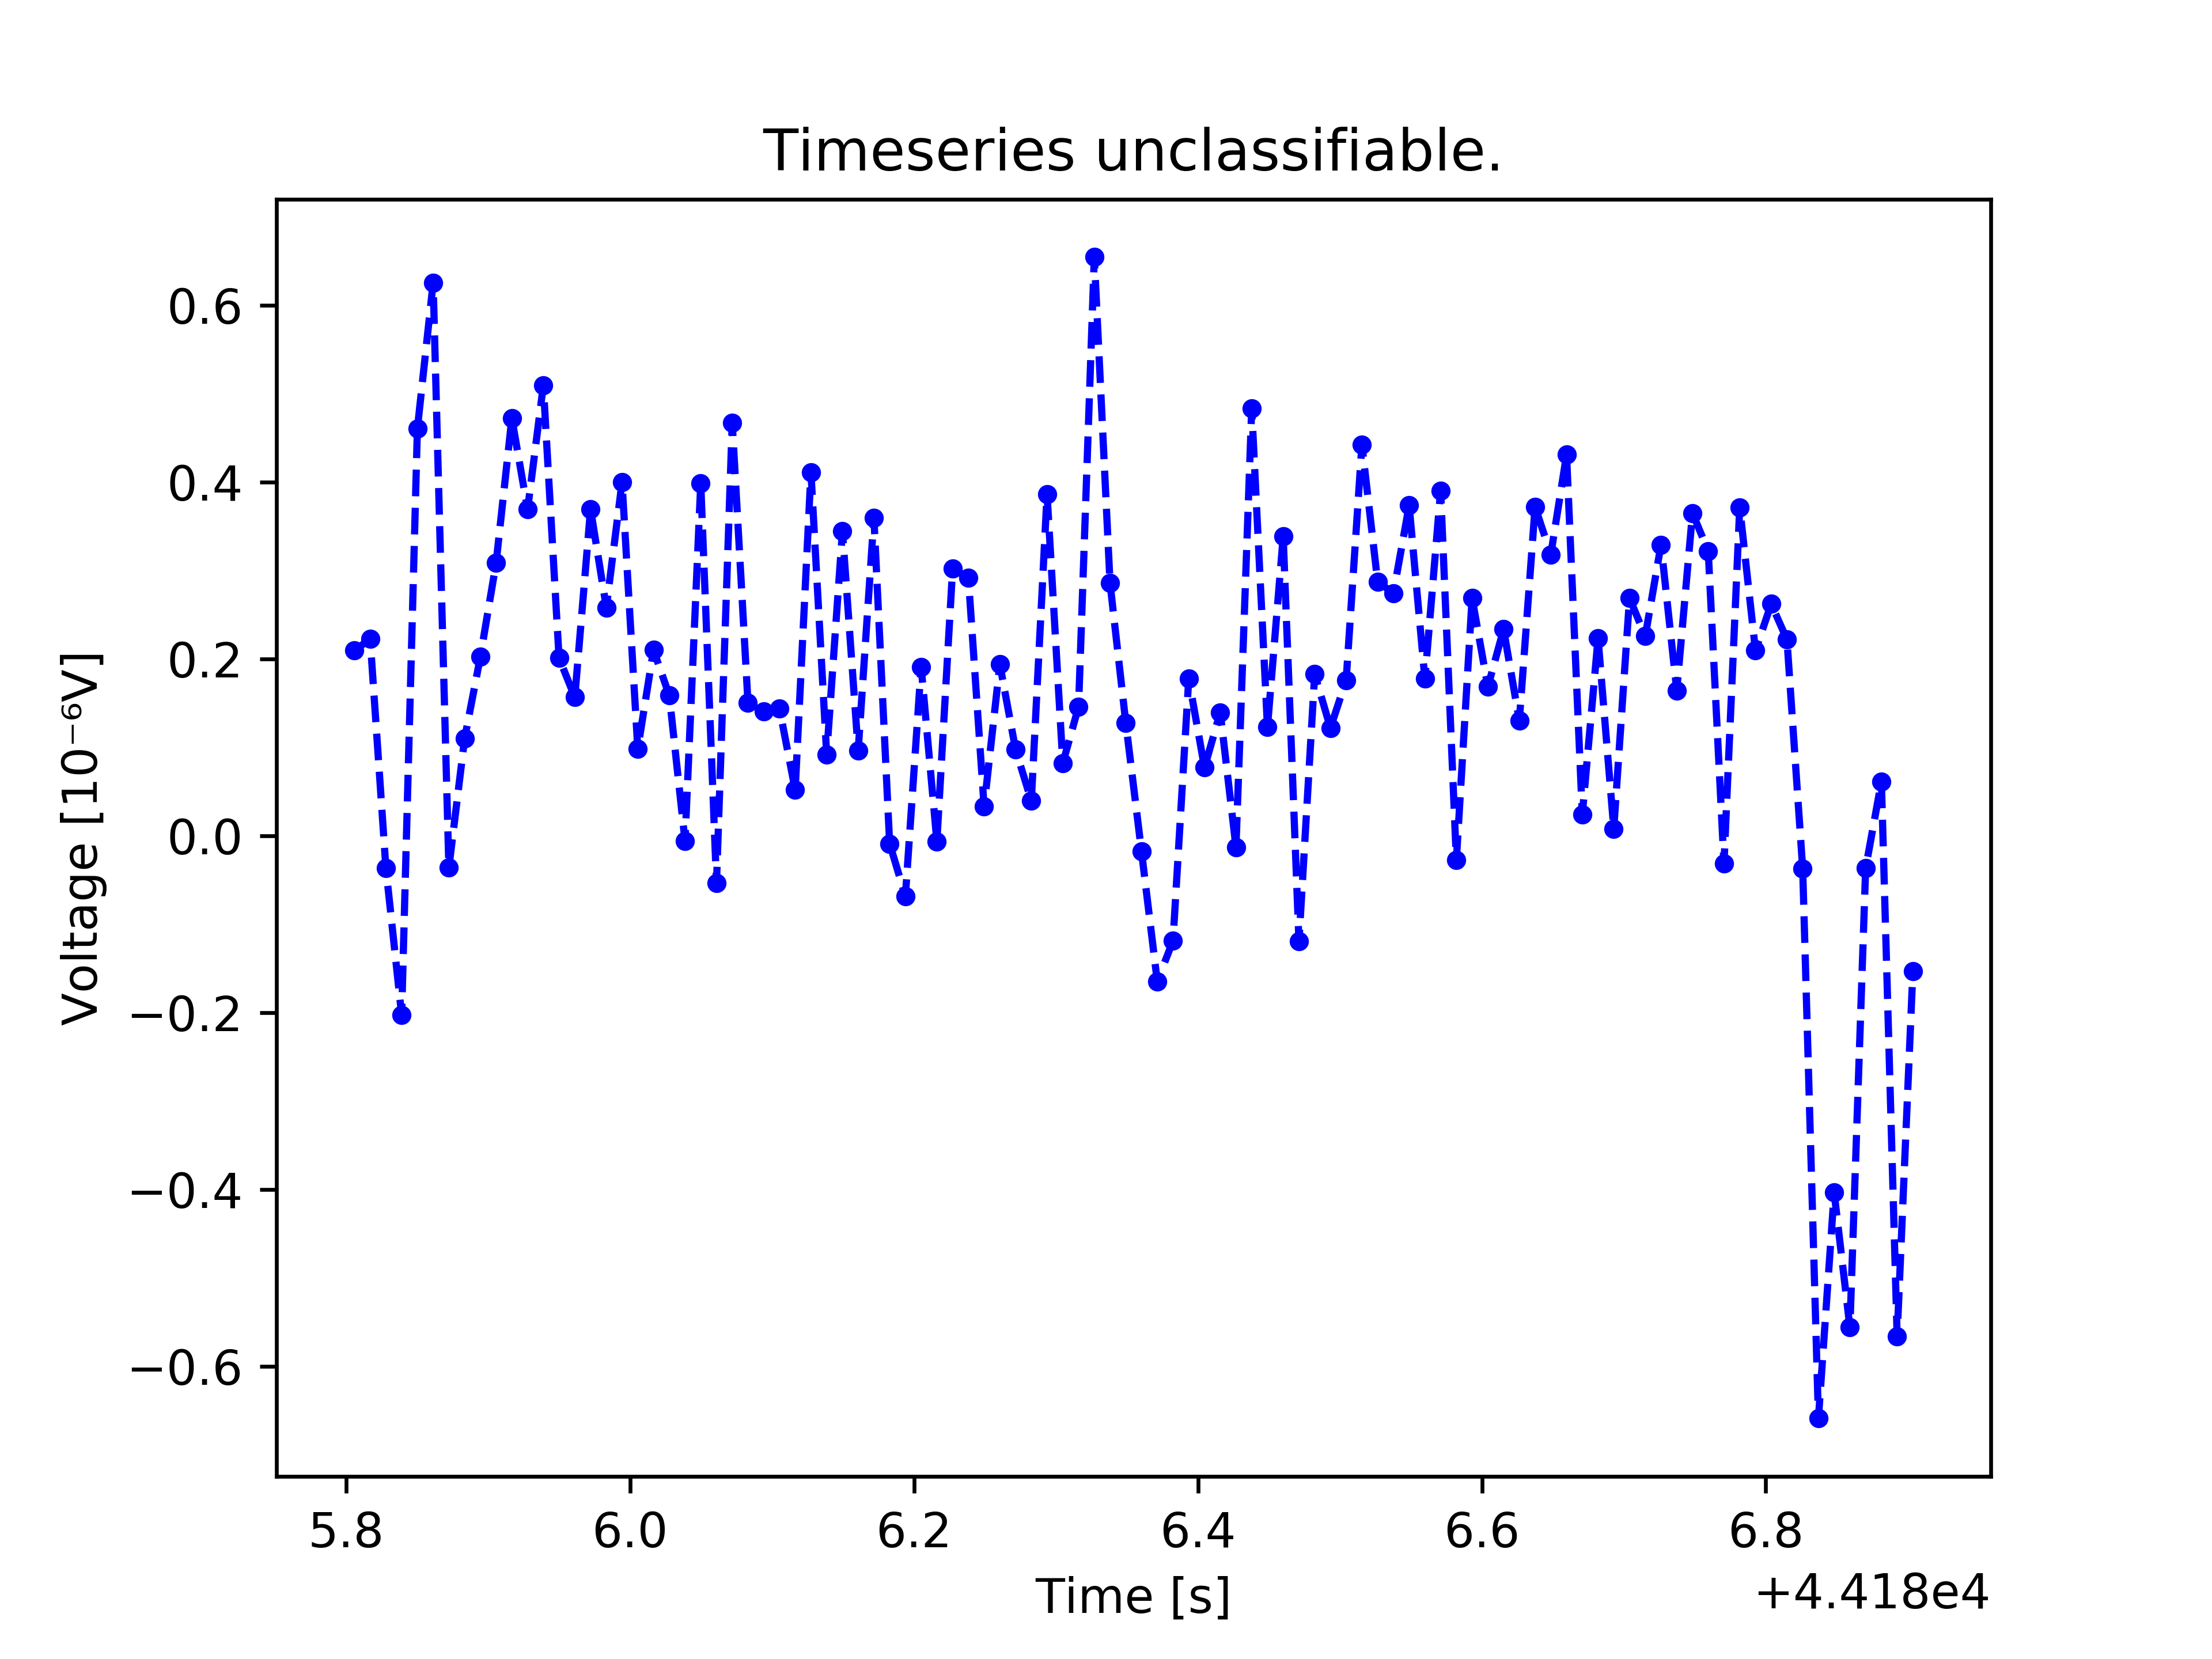
\includegraphics[scale=0.5]{figures/unclassifiable.png}
					\caption{An example of a timeseries that was not taken into consideration for the training of the network. In this case, it was not immediately evident if there was a glitch or not, so I discarded it.}
					\label{unclassifiable_plot}
				\end{figure}
			
		%
		%
		%
		%

\chapter{Glitch Detection with Neural Networks}\label{glitch_neural_networks}
		In this chapter I describe in detail the process done in order to achieve a Convolutional Network capable of recognizing the presence of a glitch in a timeseries. 	I then show its results and achievements.
		\section{Network Training}\label{network_training}
			\subsection{Data organization}\label{organizing_the_data_for_the_network}
			Following the procedure described in the previous Section, I classified 2000 timeseries as training data for the neural network (see Section \ref{neural_net}), all from a single batch of data, specifically from \texttt{OD\footnote{\textit{Operatiornal Day}. OD 01 represents the first day of operation of the satellite, which was the day of launch.} 93} bolometer \texttt{1a} ($100~\unit{GHz}$). 
			As mentioned previously, I preferred to work only with one set of data for the sake of simplicity.
			
			Before building the network, I had to prepare the test data, classified as described in Section \ref{data_classification}, in a way that could be easily fed to the network. Indeed, one of the most important tasks when using machine learning is the way the data is ``fed" into the system.			
			
			In my case, I generated two tensors, one with a binary information about the voltages for each batch, with a shape of $2000 \times 100$,\footnote{The actual number of points used where slightly less than the 2000 classified (1964), for some of them were utilized for a quick check at the end of the training.} and one with the information about the nature of every single batch (1: \textit{glitch}, 0: \textit{non-glitch}).
			The tensor containing the information about the voltages, which I call \texttt{train\_x}, has 2 indexes:
			\begin{itemize}
				\item The first one is the total number of points used for the training (2000, as said above).
				\item The second one is the number of points in each timeseries, as chosen while doing the \textit{Data Classification} (see Section \ref{data_classification}).
			\end{itemize}
			
			Then I shuffled the classified data, to avoid the network getting stuck in the wrong classification: indeed, when one inputs first all \textit{glitches} and then all of the remaining \textit{non-glitches}, the network has a hard time training.
			While working on it, I have found that, in most cases, the network was not able to learn from data that was not randomly shuffled due to too low difference between one batch and the next.
			
			\subsection{Network building}\label{network_building}
			I built the network itself using \texttt{Python} library \texttt{Keras}. Listing \ref{scripts/network.py} shows the script I used. I shall now explain the logic behind the choices for its construction and the description of its parts.
			\insertcode{scripts/network.py}{Structure of the network as written in \texttt{Python}.}
			\begin{itemize}
				\item In the first line of code, I have specified the type of general architecture that I have used. For the \texttt{Keras} library, only two specifications are possible: 
				\begin{itemize}
					\item \texttt{Sequential}, as the one I have used, which allows to build the network using \textit{blocks} added sequentially.
					\item \texttt{Model} class, used to build the \textit{Keras functional API}.  \footnote{From the Keras Documentation website, $2019$. url: \texttt{https://keras.io}.}
				\end{itemize}
				\item Following the first declaration, the subsequent lines of code implement the \textit{building blocks} of the network. As described in Section \ref{convnet}, I have used a \textit{Convolutional Neural Network}; hence, the initial layer is a \texttt{conv1D}, a one dimensional convolutional layer. 
				
				As for the number of features (\texttt{FEATURES}) and the size of the kernel (\texttt{KERNEL}), I will show later the way they were optimized for this task.
				Their best values evaluated have been:
				\begin{center}
					\texttt{FEATURES = 8}\\
					\texttt{KERNEL = 1}
				\end{center}
				\item After the definition of the first layer, a \textit{MaxPooling} was added. Being a \textit{Global Max Pooling}, its role consists in extracting the maximum value out of all the features for each channel. This is a crucial step to recognize the presence of a \textit{glitch} (hence spike) or not: a batch of data with a \textit{glitch} will present, generally, a higher maxpooling value than a \textit{non-glitch} one. 
				\item The \textit{dropout layer} in \texttt{line 12}, ensures that the network does not get stuck in some wrong classification.
				\item The job of the last 2 softmax-activated \textit{Dense} layers is to learn as much extra information as possible from the output of the pooling layer. The last one implements a sigmoid: this ensures that the output is a number between 0 and 1, representing the probability to find a \textit{glitch}.
			\end{itemize}
			The architecture described above is the most efficient I was able to find. Its form and shape is the result of various trials and tests, starting from a simple 2 layer code to begin with. 
			Unfortunately, as of today, Data Science does not have a general algorithm to construct the best network for each situation: most of the times, just like I did, one starts from some known base module and builds upon it, trial after trial, trying to find the, hopefully, perfect fit.			
			
			I would like point out how this research for the correct network is often full of weird and new mistakes, which renders the search sometimes quite long and unpredictable. In my case, I found a textbook example of \textit{data types problems}: as one can see from most of the graphs reported in this thesis, the values I had to work with were voltages in the order of $10^{-6}$ or less. While this does not seem to be a huge computational problem in modern \texttt{64-bits} computer architectures, the library I used was, for optimization reasons, built around \texttt{32-bits} floating point numbers: not knowing this fact, I spent many hours trying to figure out why the output of the network was completely random. Indeed, what was happening was that the program, not being able to read \texttt{64-bits} numbers, truncated my data, most of the times to $0$: this made for a completely random output to be generated, which for a long time eluded my understanding. 			
			
			The following logical steps I took was to compile with some parameters the network and then to run the training using the data I prepared.
			In the compilation of the network, it is vital to specify 3 characteristics, which define how the training will be done:\cite{chollet}.
			\begin{itemize}
				\item The optimizer, whose role is to tell the network how to improve the parameters. I choose \texttt{rmsprop}.
				\item The loss, which specifies a function whose calculated value, for each step, is the parameter the network has to optimize. Because of the binary classification, I choose \texttt{binary crossentropy}.
				\item The metrics is a function which outputs how well the training is going; I choose \texttt{accuracy}, hence a number between 0 and 1, the ratio between the number of timeseries classified correctly and the total number of datasets.
			\end{itemize}
%			While the functions we used are, to someone who is trained in machine learning, very common and simple, they ended up being the best solution for our network. In this non-trivial choice, we decided to follow the guidelines highlighted by Dr. Chollet in his book 			
			
			Once the data had been prepared and the network compiled, I trained it. The free parameters I had to set to do the training are the batch size to use (\texttt{BATCH}) and the number of epochs on which to train (\texttt{EPOCHS}). The variation in the batch size can make the learning process either very efficient or not; the number of epochs must be so that it is not too small or too large. In the first case, the network would not have enough time to learn the correct features; in the latter, training for too long could end up having your data \textit{overfitted}. 			
			
			Again, I choose these two parameters using the method described below; I report the values which gave the best results:
			\begin{center}
				\texttt{BATCH = 10}\\
				\texttt{EPOCHS = 40}
			\end{center}
			Before training, I also decided to use some data as \textit{validation}:  having some sort of validation allows to see how, step by step, the network works on unseen timeseries. It is also a good instrument to check on the presence or not of \textit{overfitting}. I took $20\%$ of the training data as validation, hence I trained the network on 1600\footnote{Again, slightly less, as said previously.} timeseries.
			
			\subsection{Optimization of the network parameters}\label{optimization_of_the_network_parameters}
			%
			%		NOTE: Non so se mettere questa sottosezione in questa sezione oppure nella successiva.
			%
			
				As mentioned in the previous two sections, Section \ref{organizing_the_data_for_the_network} and \ref{network_building}, I devised a way to optimize all of the numerical parameters present in the \textit{Network}. I summarize here the technique  followed. 				
				
					The best and most effective way to find the fittest parameters would be to run the training for all possible configurations and then find which one yields the best results. While it would be the best approach, in practice, with the apparatus I had, it is almost impossible to achieve: with a conservative estimate, it would take more than one year to do the whole calculation.\footnote{All of the calculations in this thesis have been made using a normal computer laptop CPU. During a bigger, and with more budget, application of the techniques described in this work, one might be able to run all of this using CUDA-GPUs, which can dramatically improve the time of execution. \cite{cuda-gpu}}
					Even though I could not use a complete optimization as just described, I managed to do some \textit{partial optimizations}, which is far better than only trying to guess by hand. What I did was to run the network repeatedly for all possible parametrical values separately. More specifically:
					\begin{itemize}
						\item I run the network $30$ different times with a set configuration for the other parameters (\texttt{BATCH = 10, EPOCHS = 40} and \texttt{FEATURES = 1}), trying to find the best kernel size between $1$ and $30$. Fig. \ref{optimization_plot_kernel} shows the results obtained. In this case, the higher the dimentionality of the kernel, the worst the accuracy of the network. 
						I chose to use \texttt{KERNEL = 1} as my final choice for this variable.
						\item I run the network $30$ times to find the best configuration for the number of features. As shown in Fig. \ref{optimization_plot_features}, the dependence of the accuracy on the number of features is almost negligible. I still took the best accuracy as a way to chose the value to use, which yielded
						\begin{center}
							\texttt{FEATURES = 8}
						\end{center}
						As for the other parameters, I used the same as in the previous optimization, and with the kernel size as previously found.
						\item The last parameter I optimized was the batch size: as in the previous two cases, I ran the network multiple times (120) and used the validation accuracy to weight my choice. As one can see in Fig.  \ref{optimization_plot_batch}, even in this case there is little to zero dependence on the size of the batch relative to the accuracy of the network.  
						This time I preferred not to use the best actual result (which corresponds to $41$), but I decided for \texttt{BATCH = 10}. The reason behind this choice is merely computational time: a big batch means that, in order to reach a good accuracy, it will take a larger number of epochs. Given that the difference between of all these results is very small (of the order to $10^{-3}$), I preferred to avoid a larger computational time.
						Again, for the other parameters in the network, I used the same configuration as above.
					\end{itemize}
					
				  \begin{figure}[h!]
				        \centering
				        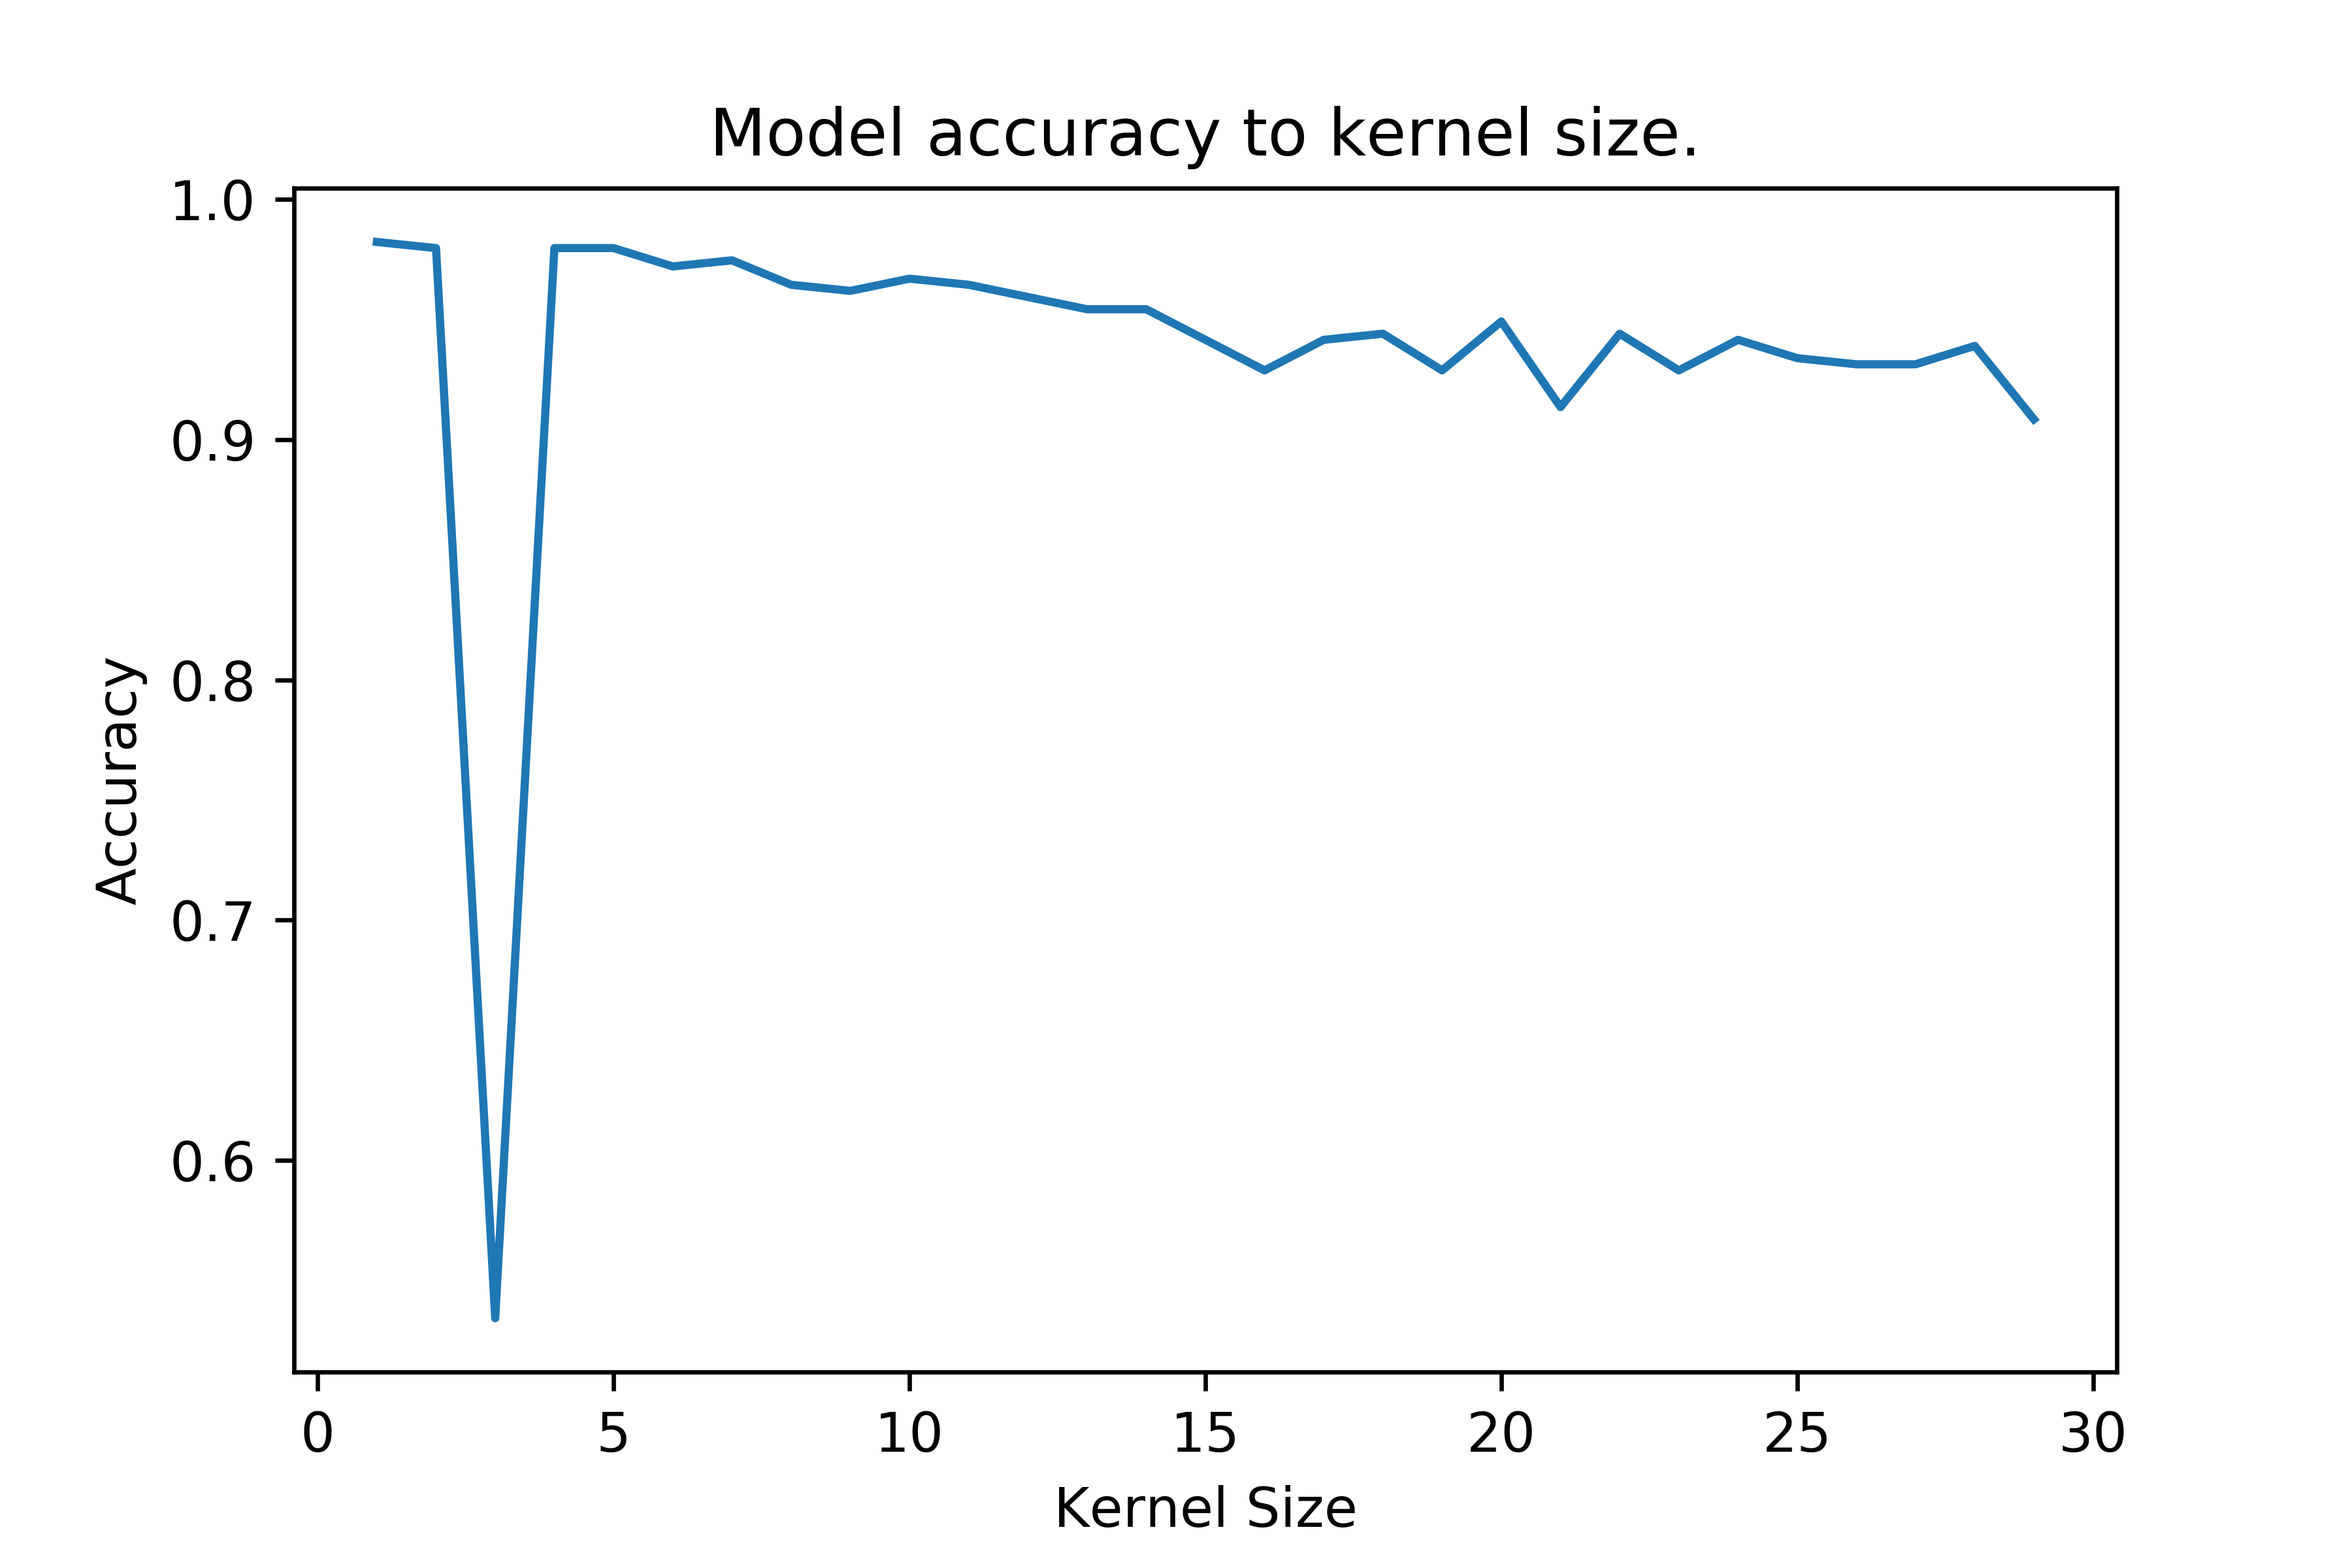
\includegraphics[scale=0.5]{figures/kernels.png}
				        \caption{Validation accuracy for the last epoch (run with $30$ epochs) for different values of the kernel size. The accuracy decreases as the size grows. \\
				        For the kernel size $3$, the accuracy suddenly drops below $60\%$: this is due to \textit{overfitting}. For some unknown factors, for that specific run, with the values given, the network would get ``stuck" and overfit.}
			    \label{optimization_plot_kernel}				        
			    \end{figure}%
			  
					The parameter \textit{accuracy} used to optimize all of these variables was taken to be the accuracy for the validation data in the last epoch. Even though in some cases it might not be the best general fit, I found that it is the most effective one. Indeed, taking the training accuracy instead could have given rise to problems if the network would have gone into \textit{overfitting}; with my choice, I had a parameter which could actually tell  how the network is generally going, while being able to avoid \textit{overfitting} problems. 					
					
					I did however encounter some small problems, which I have not  managed to solve completely. Looking, epoch after epoch, at the validation accuracy for some of the last epochs in each training, I discovered how said parameter could fluctuate by up to $2$ percentage points in its value. Where this happened, I still preferred to work with my choice. In such cases, there is a small chance for the \textit{true} best value to be different than the one chosen; but, as I have tested in my many trials, my result is not too much different and yields almost the same overall result in the final training.
					\begin{figure}[h!]
					\centering
			        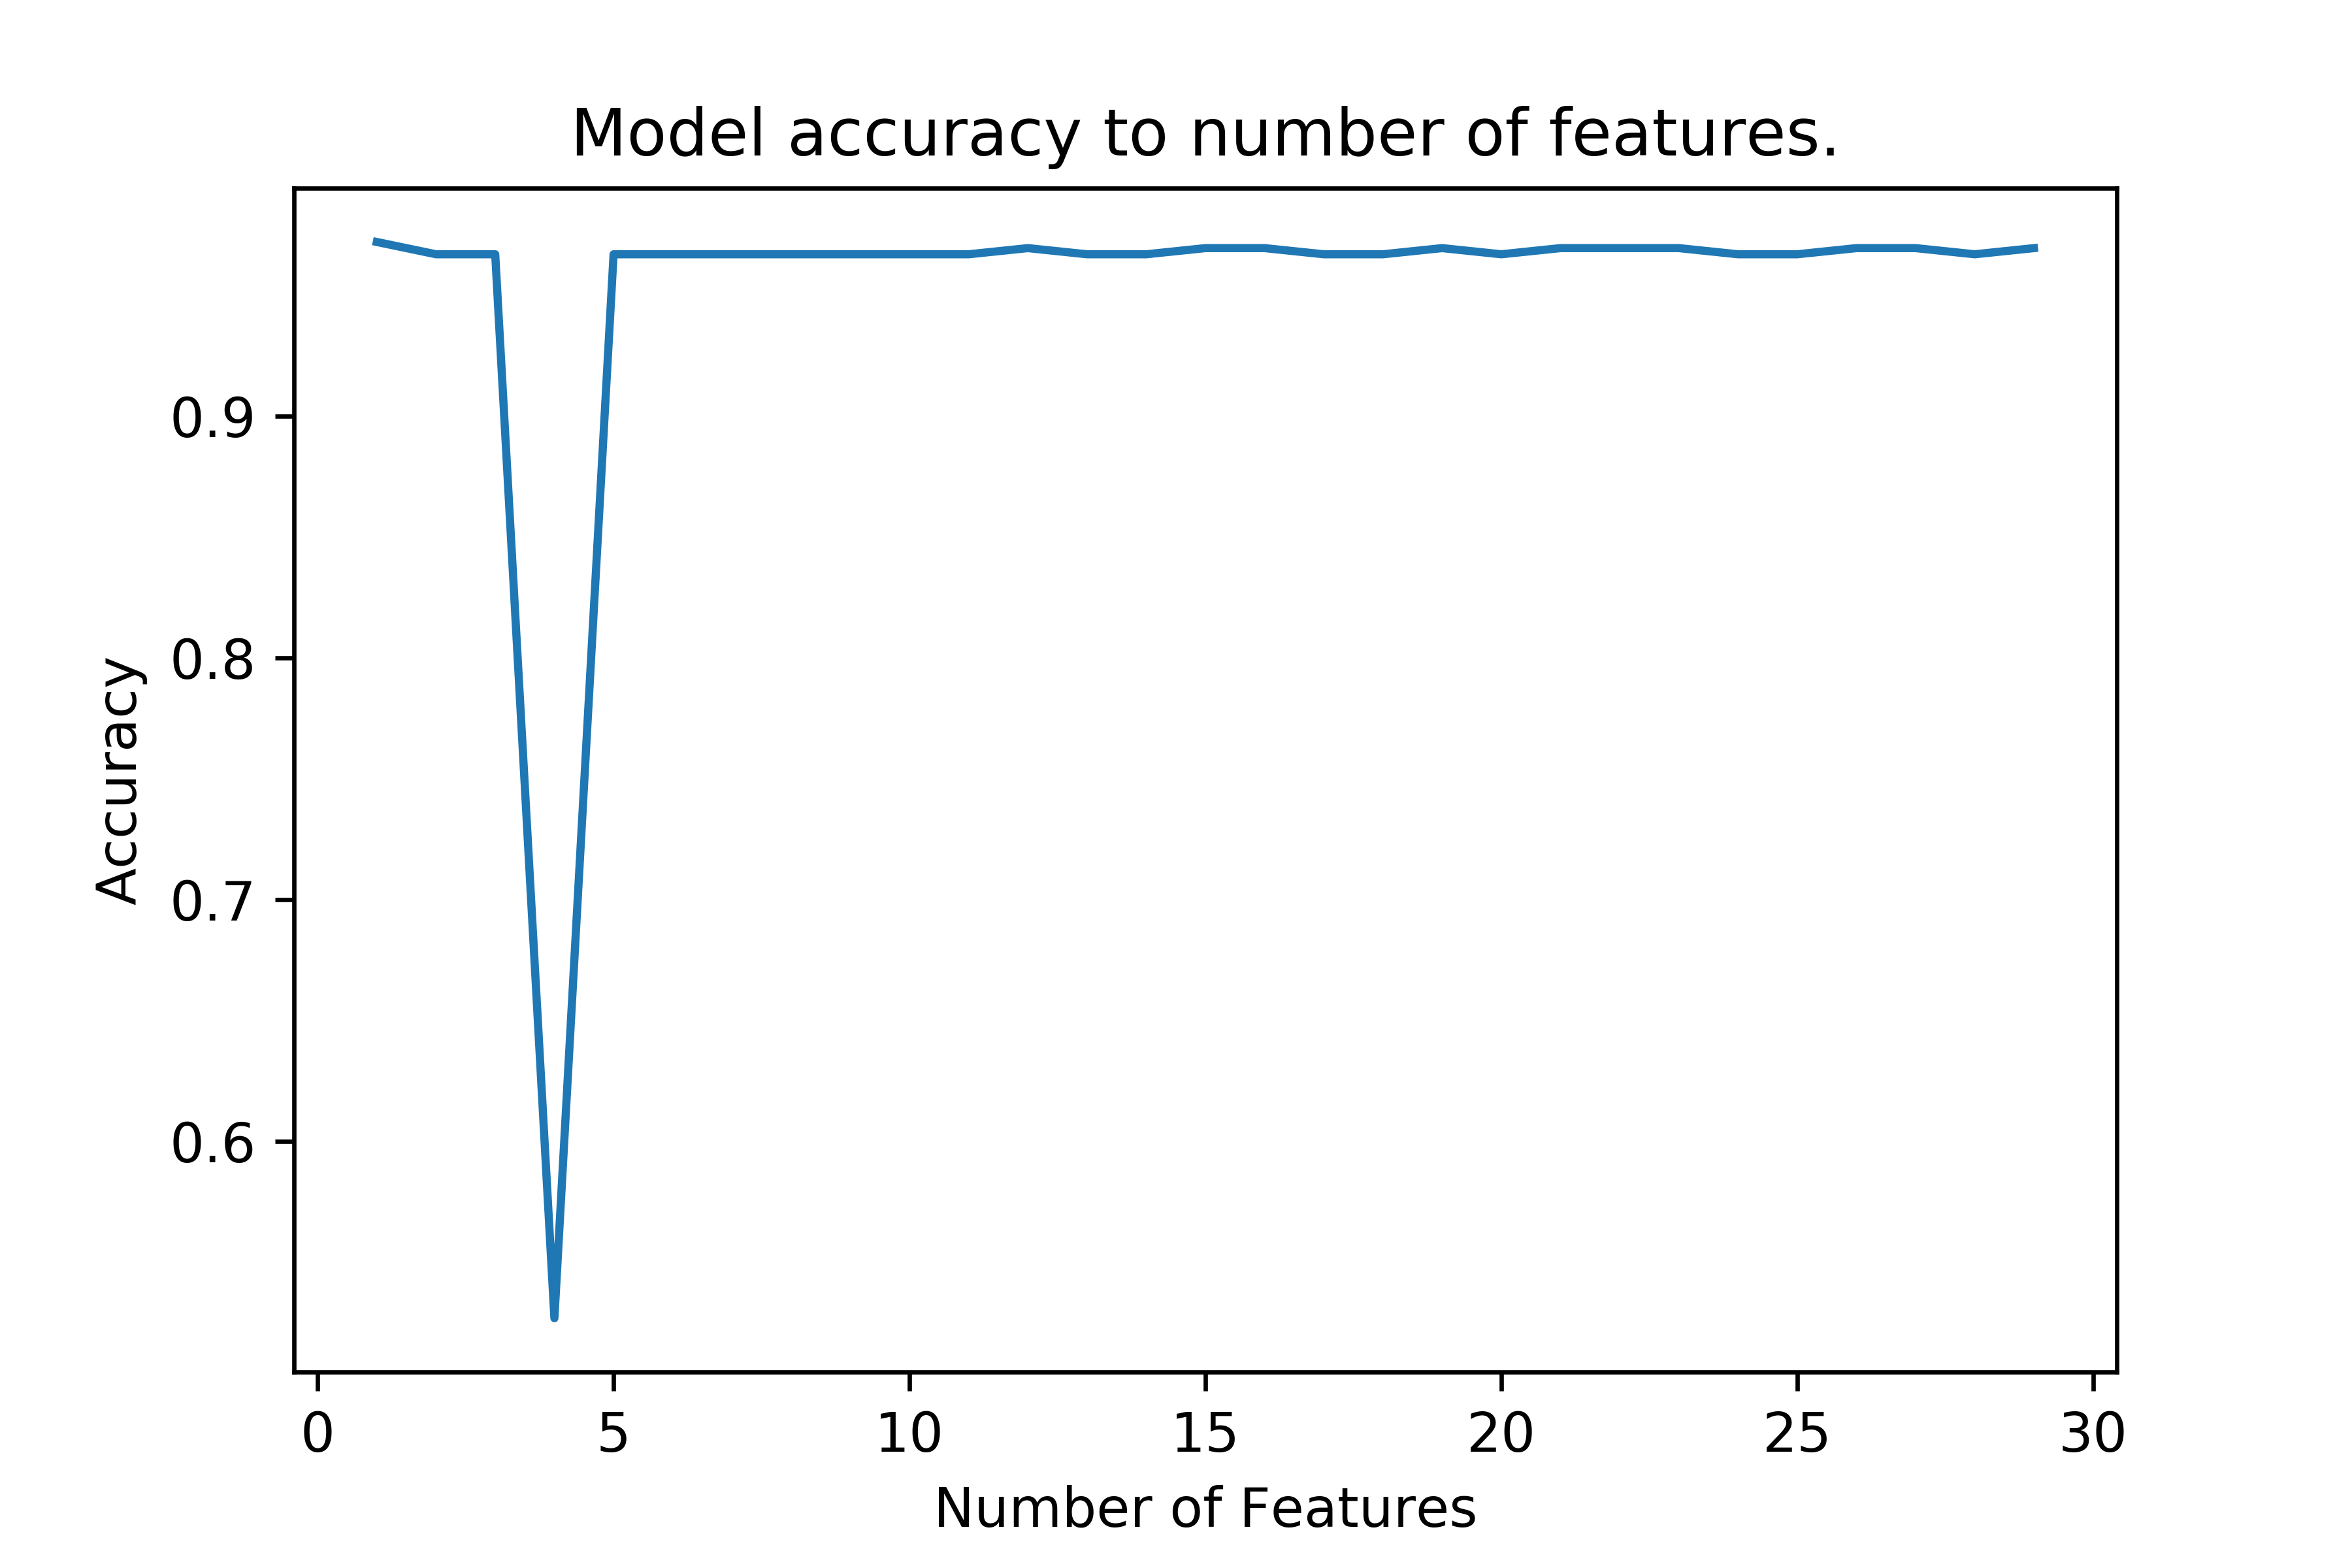
\includegraphics[scale=0.5]{figures/features.png}
					\caption{Validation accuracy as a function of the number of features. The accuracy almost does not change with the change in the number of features.\\
					As in Fig. \ref{optimization_plot_kernel}, for a certain value of \texttt{FEATURES}, the network overfitted, resulting in accuracy below $60\%$.}
			    \label{optimization_plot_features}					
			    \end{figure}
			    
			    \begin{figure}[h!]
					\centering
			        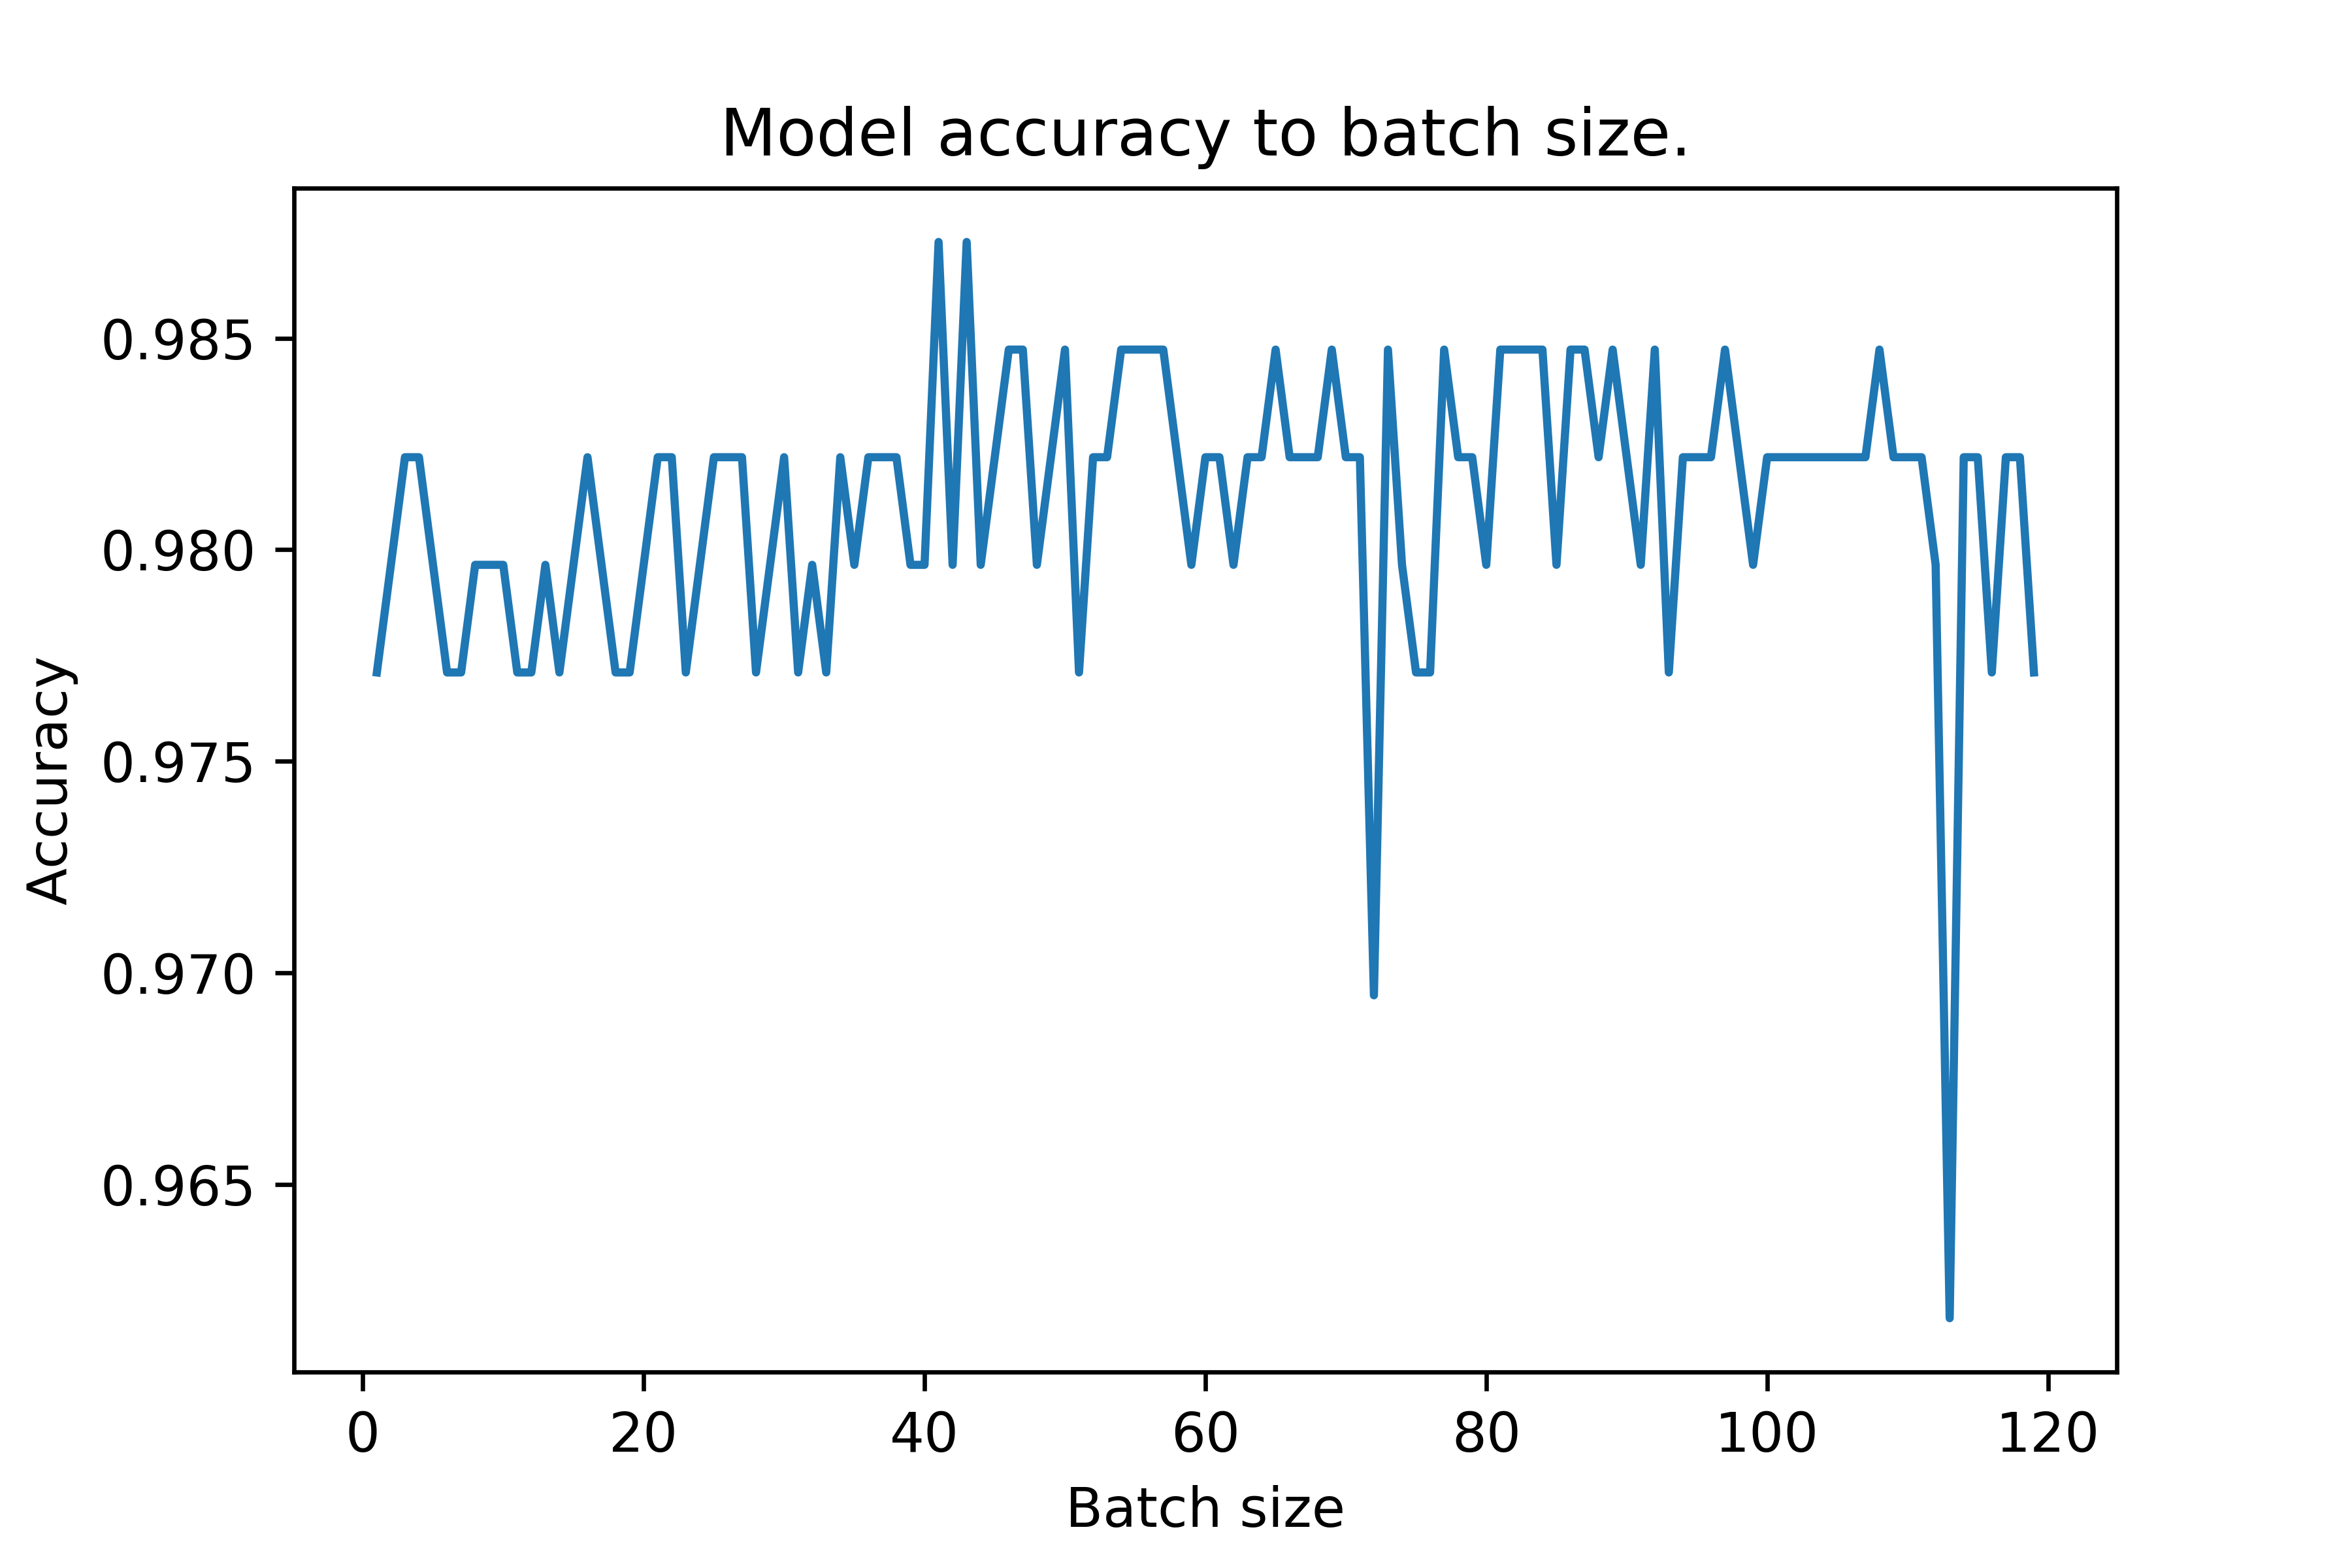
\includegraphics[scale=0.5]{figures/batches.png}
					\caption{Validation accuracy to batch size for my model. Overall, the changes tend to be very small and, most likely, caused by randomness.}
			    \label{optimization_plot_batch}					
			    \end{figure}
			%
			%
			%
			%
			%
		\section{Network Results}\label{network_results}
		\subsection{Preliminary results}\label{preliminary_results}
			As mentioned, the training was done with approximately $1600$ timeseries for $40$ epochs. With the final configuration, realized with the optimized parameters, I obtained a very high accuracy, both on the training and validation sets, which almost exceeded my expectations. Fig. \ref{results_plot} shows the results for the accuracy and loss for the two sets of data. 
			
			As one should expect from a very good network, my results show that, both on the training and validation data, the accuracy (and loss\footnote{The loss and the accuracy are not mathematically related, which means their progression can be independent. \footnote{From Harshit Kumar's online blog. url: \texttt{https://kharshit.github.io/blog/2018/12/07/ loss-vs-accuracy}.}}) increases (decreases) gradually, reaching a very desirable final result of:
			\begin{center}
				\texttt{TEST ACCURACY = 97.71\%}\\
				\texttt{VALIDATION ACCURACY = 97.71\%}
			\end{center}

			\begin{figure}[h!]
						\centering
				\begin{subfigure}[t]{0.65\textwidth}
					\centering
					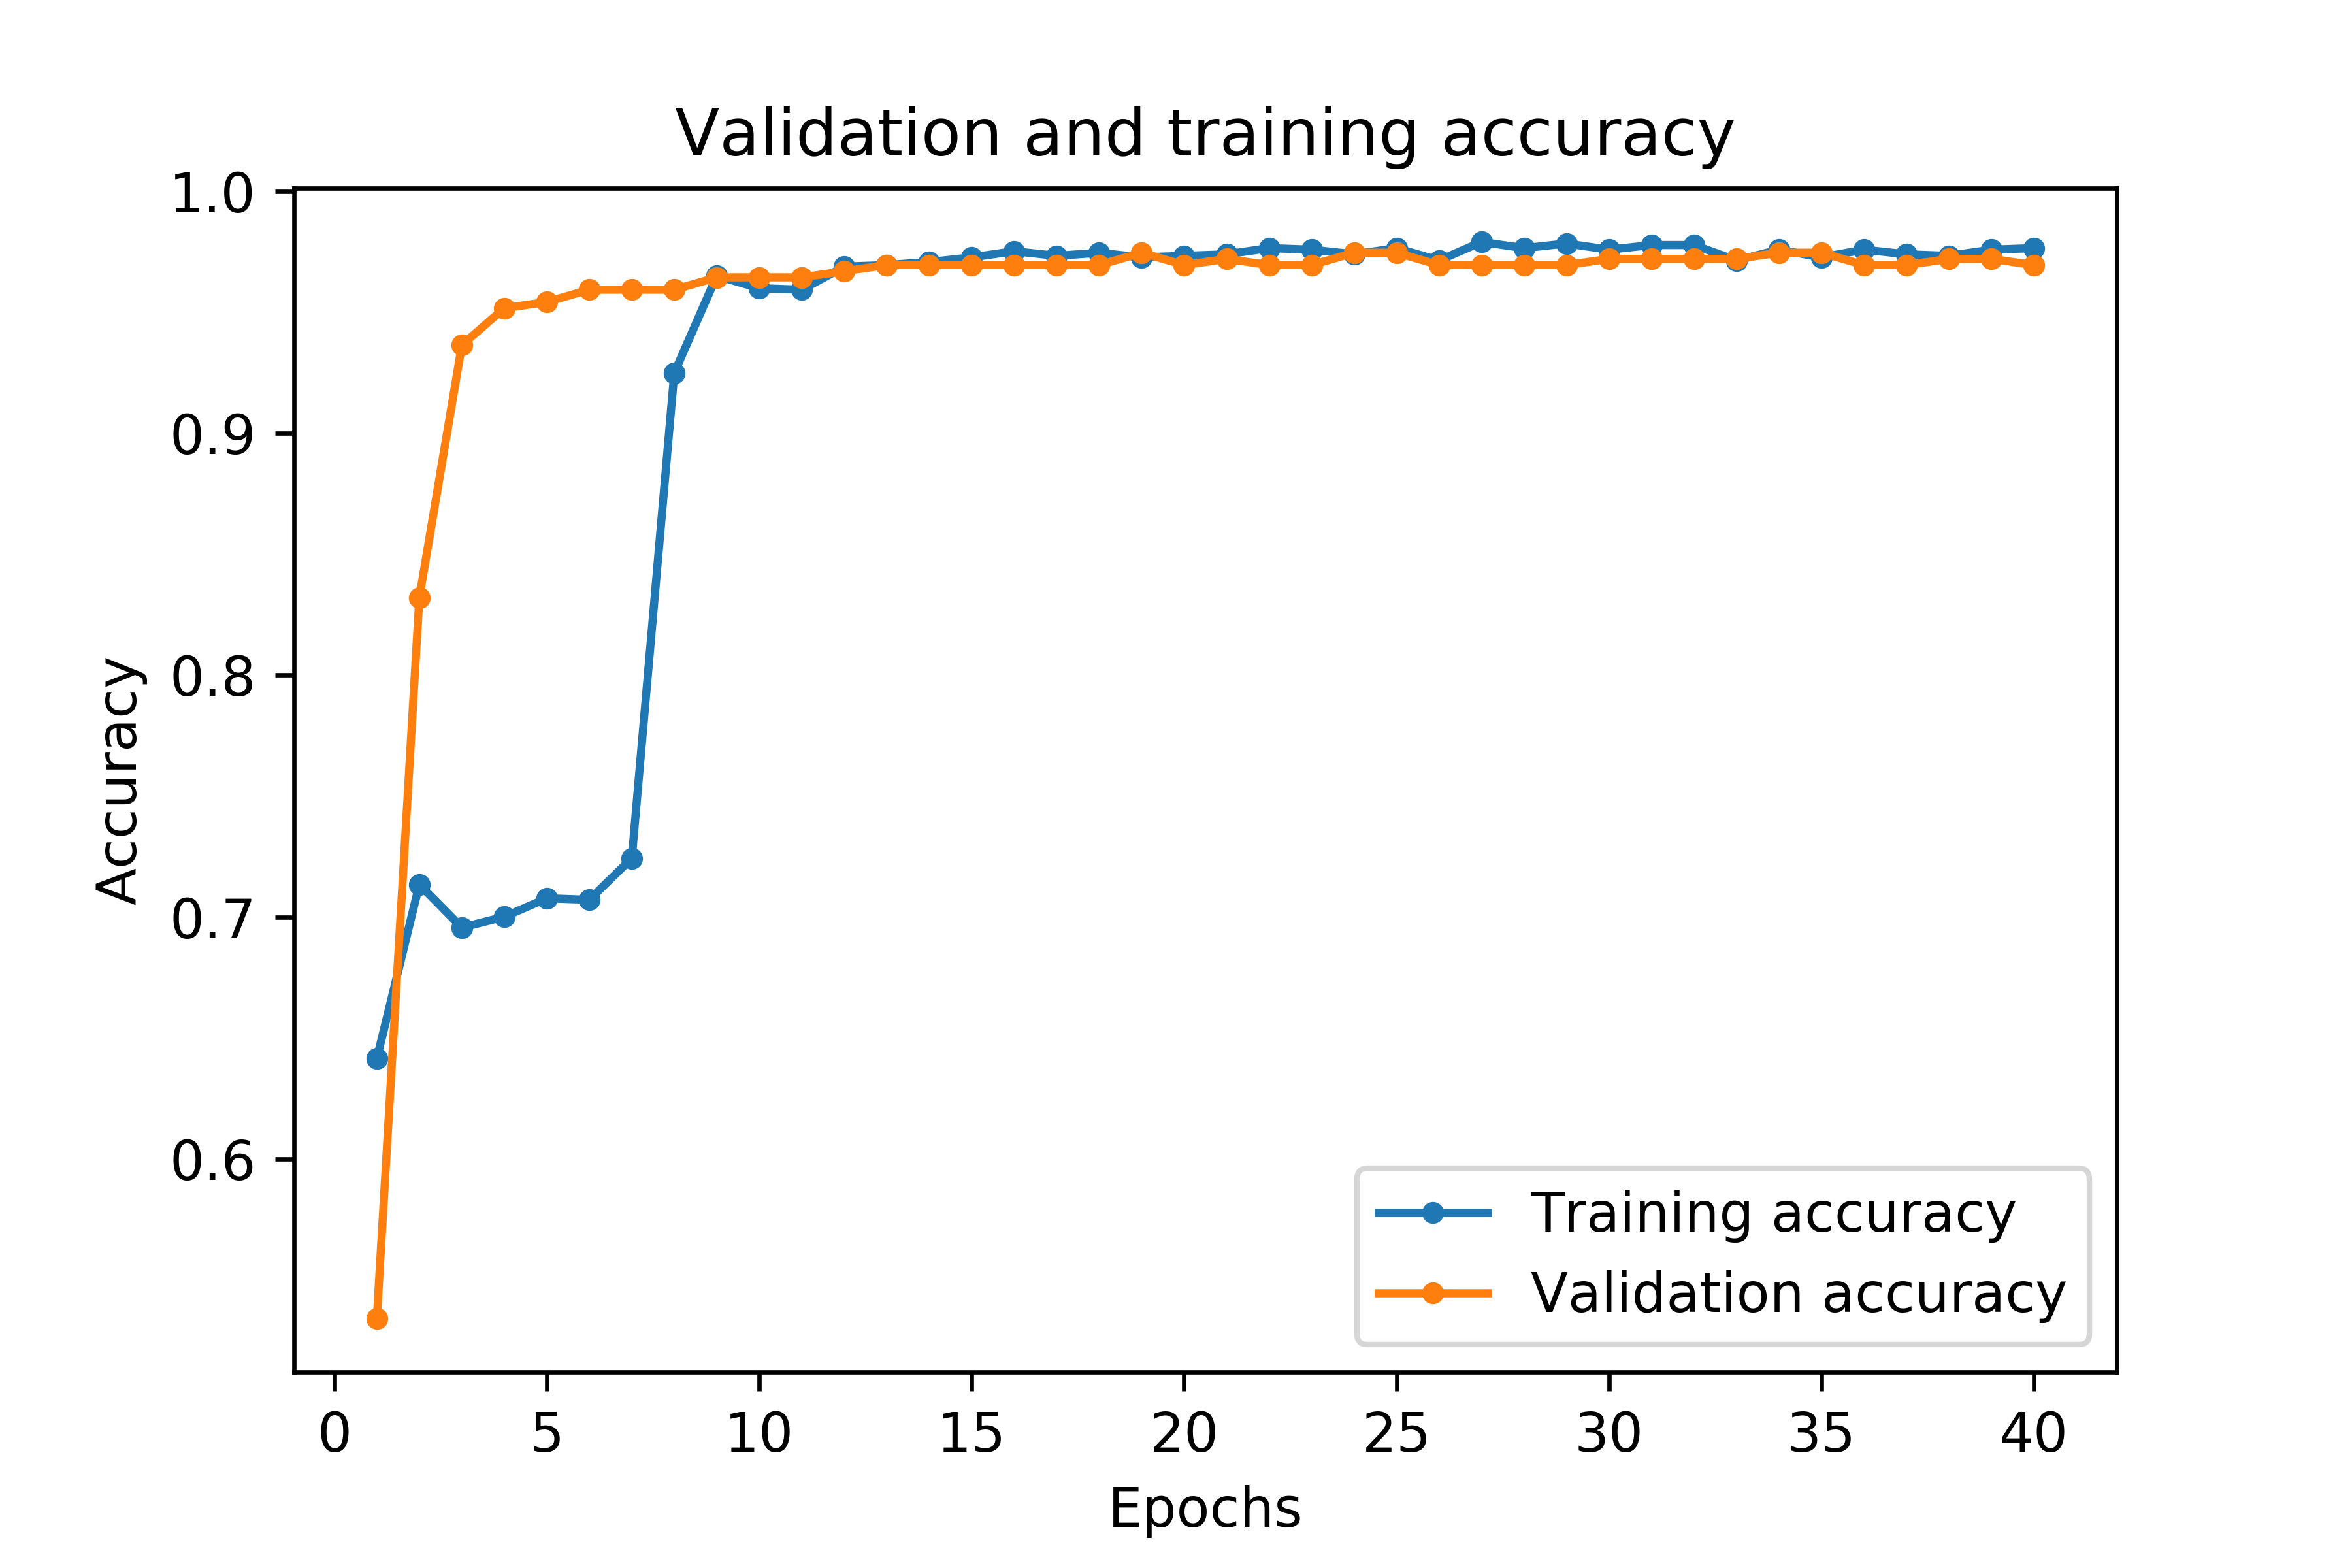
\includegraphics[scale=0.5]{figures/accuracy.png}
					\caption{The network's test and validation accuracy. After about 10 epochs, they peak and increase by a little over the following ones: the network has managed to learn all of the possible information.}
					\label{accuracy_plot}
				\end{subfigure}
				%
				%
				\begin{subfigure}[t]{0.65\textwidth}
				\centering
				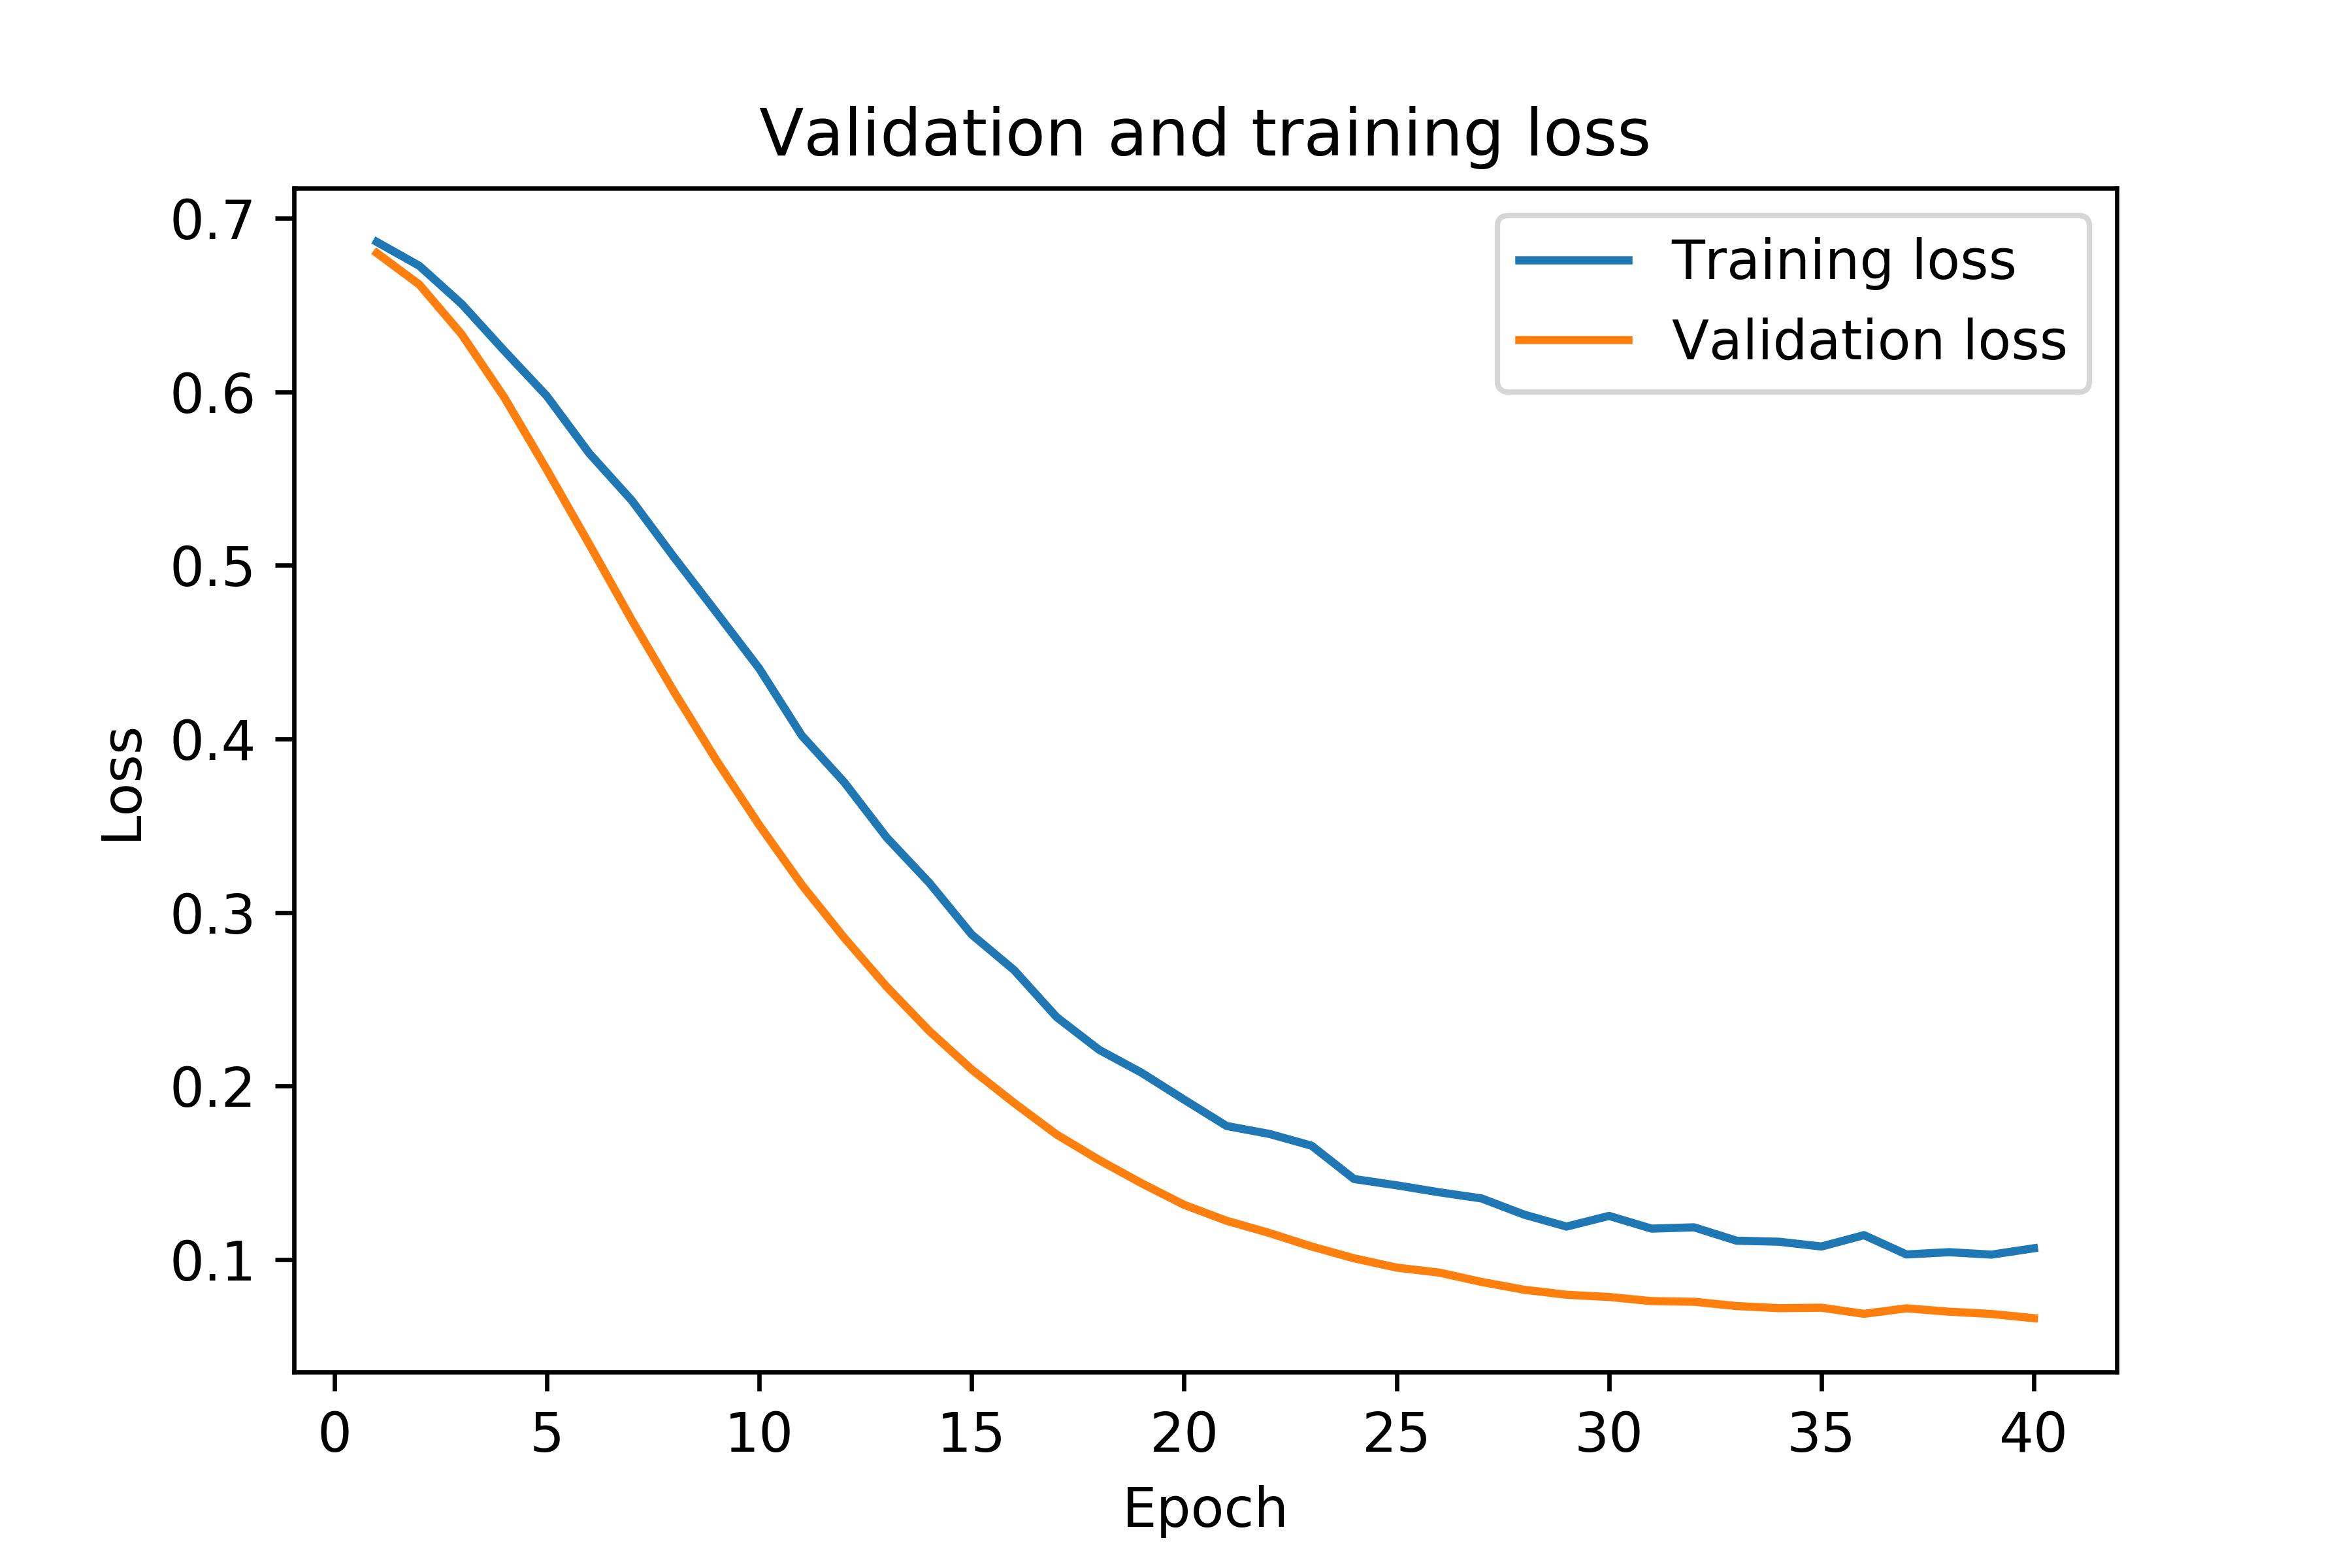
\includegraphics[scale=0.5]{figures/loss.png}
				\caption{Test and validation loss for the network. Both of them decrease over time, as one should expect; the fact that the validation loss tends to be lower is purely random and due to the smaller size of its sample space.}
				\label{loss_plot}
				\end{subfigure}
				\caption{}
				\label{results_plot}
			\end{figure}
			
			Considering that some data might have been wrongly classified, the results show how remarkable the neural network can be. 
			I also tested it on a new timeseries, which was classified by hand but neither used for the training or validation sets: the very good result is shown in Fig. \ref{fig:text_example}.
			\begin{figure}[h!]
			\centering
				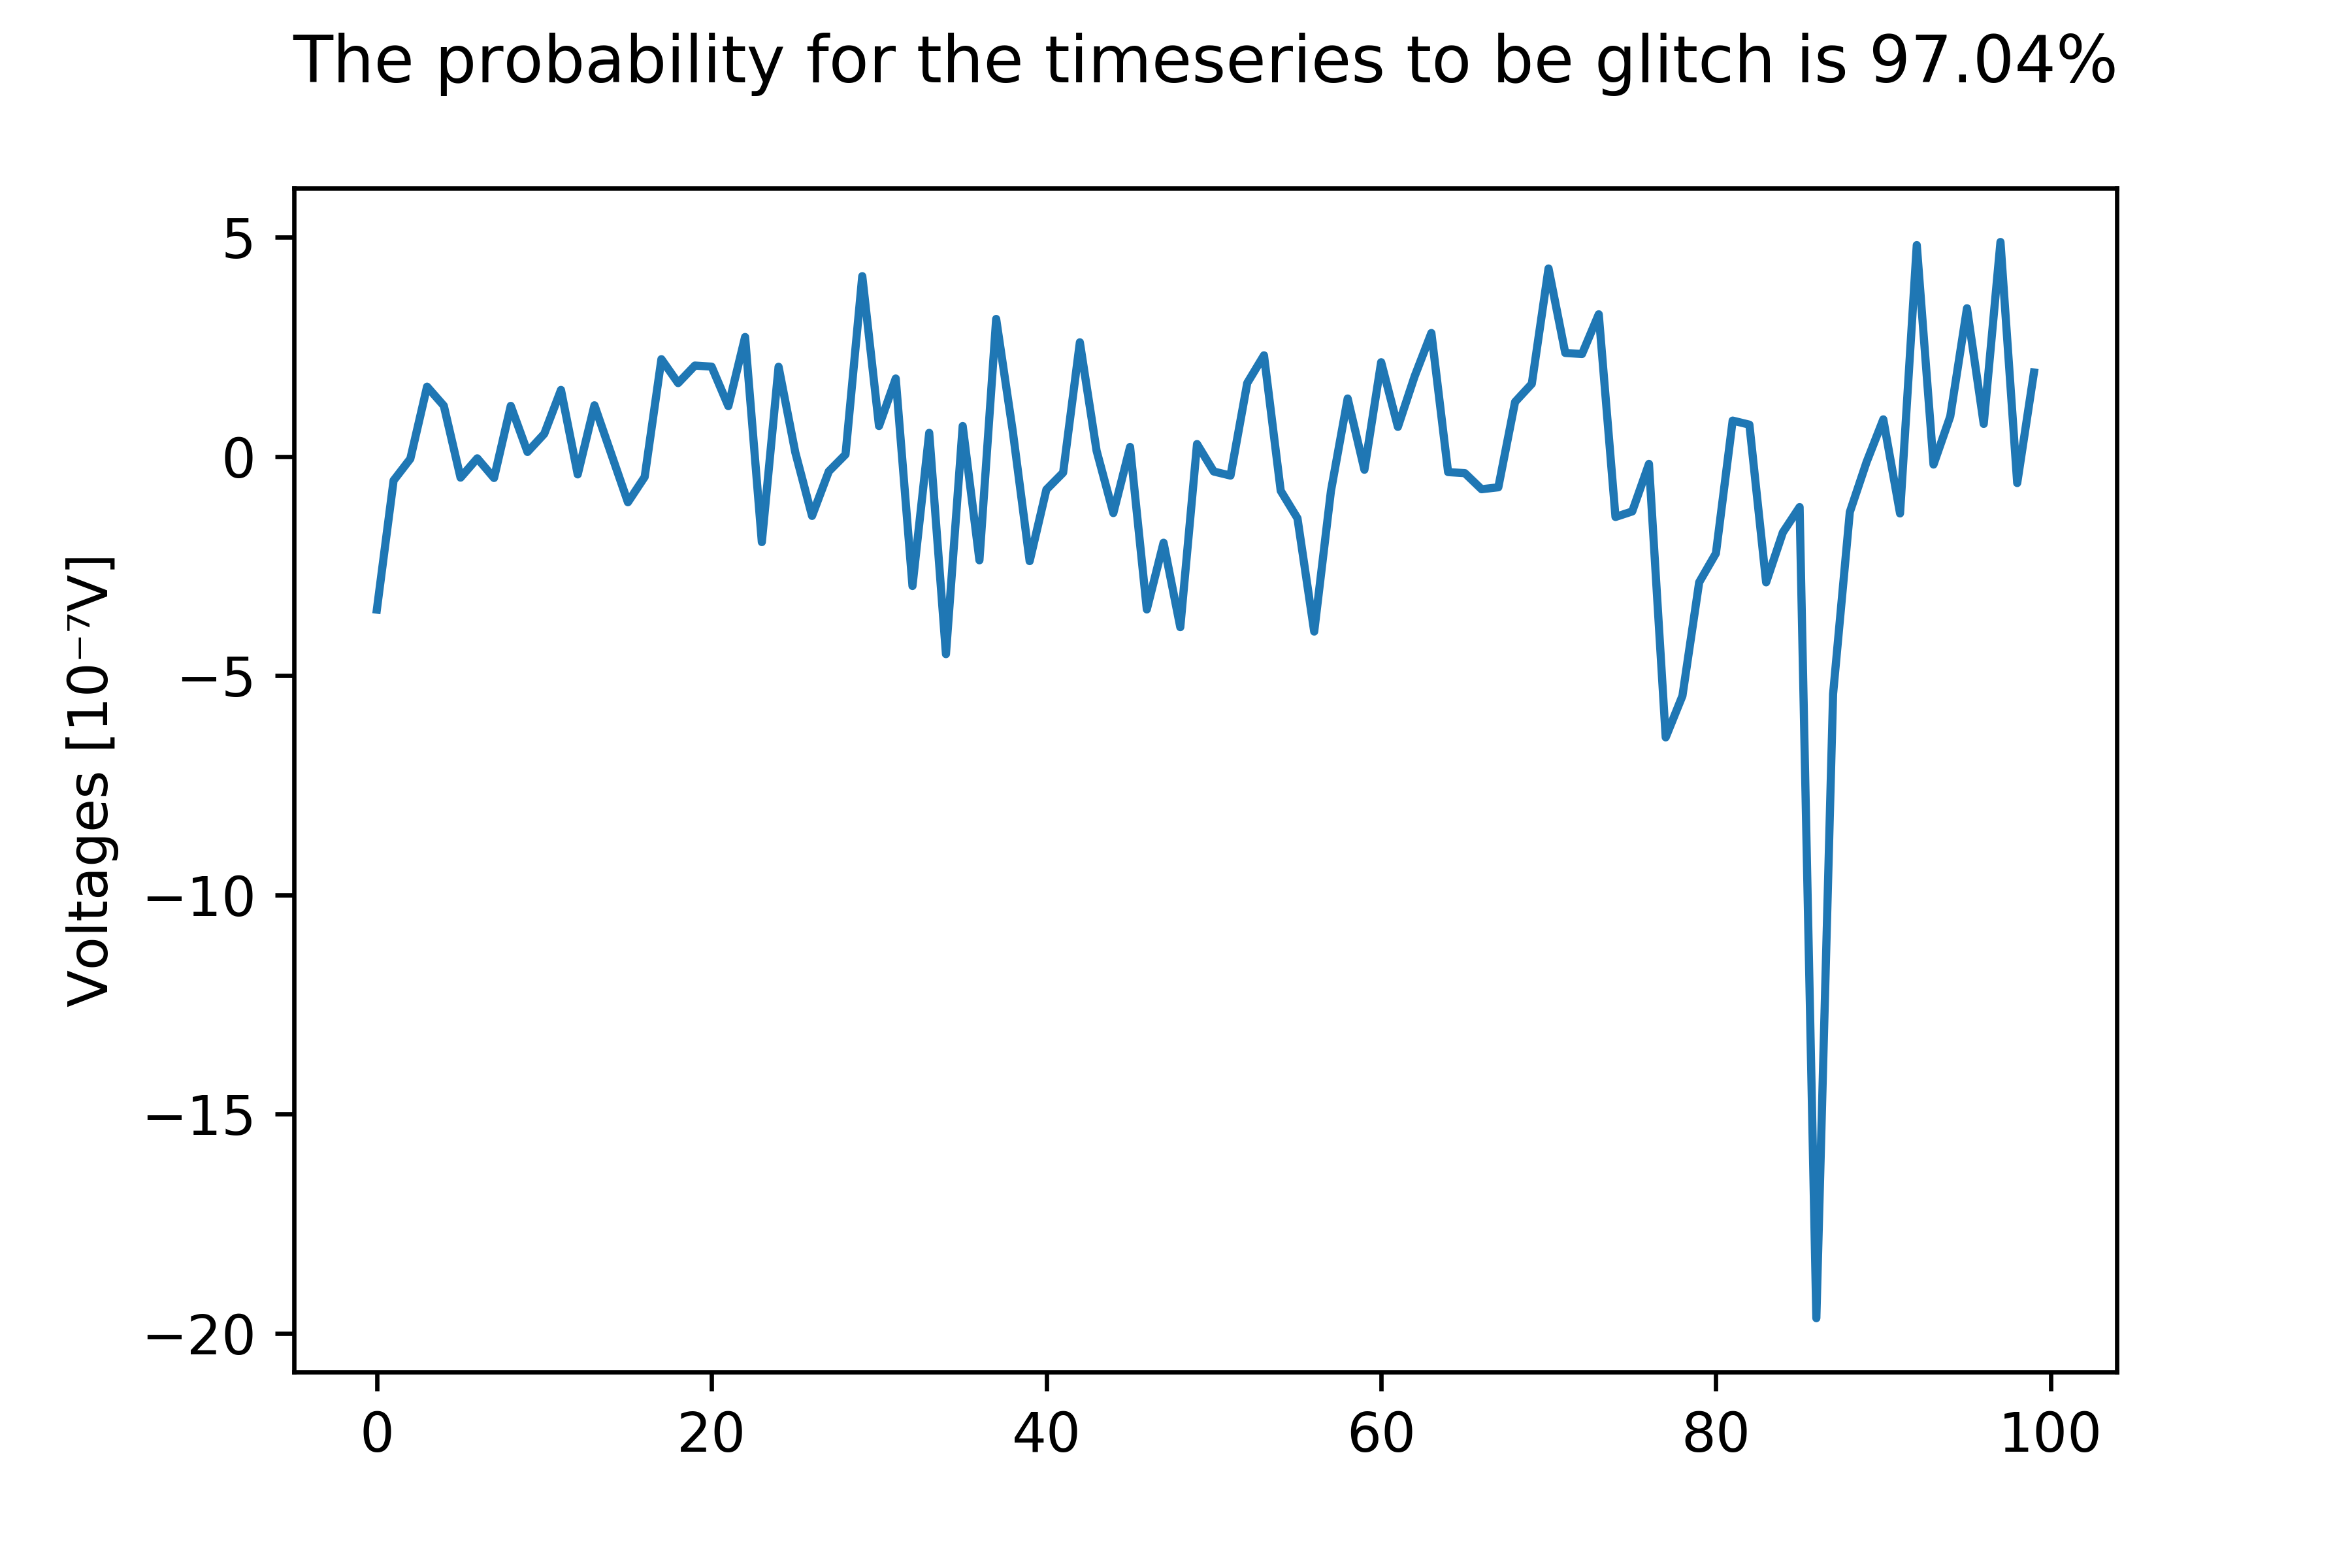
\includegraphics[scale=0.6]{figures/test_example.png}
				\caption{Example of classification of a timeseries with a \textit{glitch}. Above is the probability, given by the network, that the figure presents a \textit{glitch}; it is important to remember that the output is never perfectly 100\%, and it's up to me to determine a \textit{threshold}.\\
				The $x$-axes shows the index of each sample.}
				\label{fig:text_example}
			\end{figure}			
			
			In order to measure the \textit{power} achieved by the network, I tried it on different timeseries, both from the same batch of data as the training and validation sets and from other ones, to see how it could fare. Some examples are shown in Fig. \ref{fig:test_plot_1}, \ref{fig:test_plot_2} and \ref{fig:test_plot_3}.
			
			\begin{figure}[h!]
				
				\begin{subfigure}[t]{0.5\textwidth}
				
					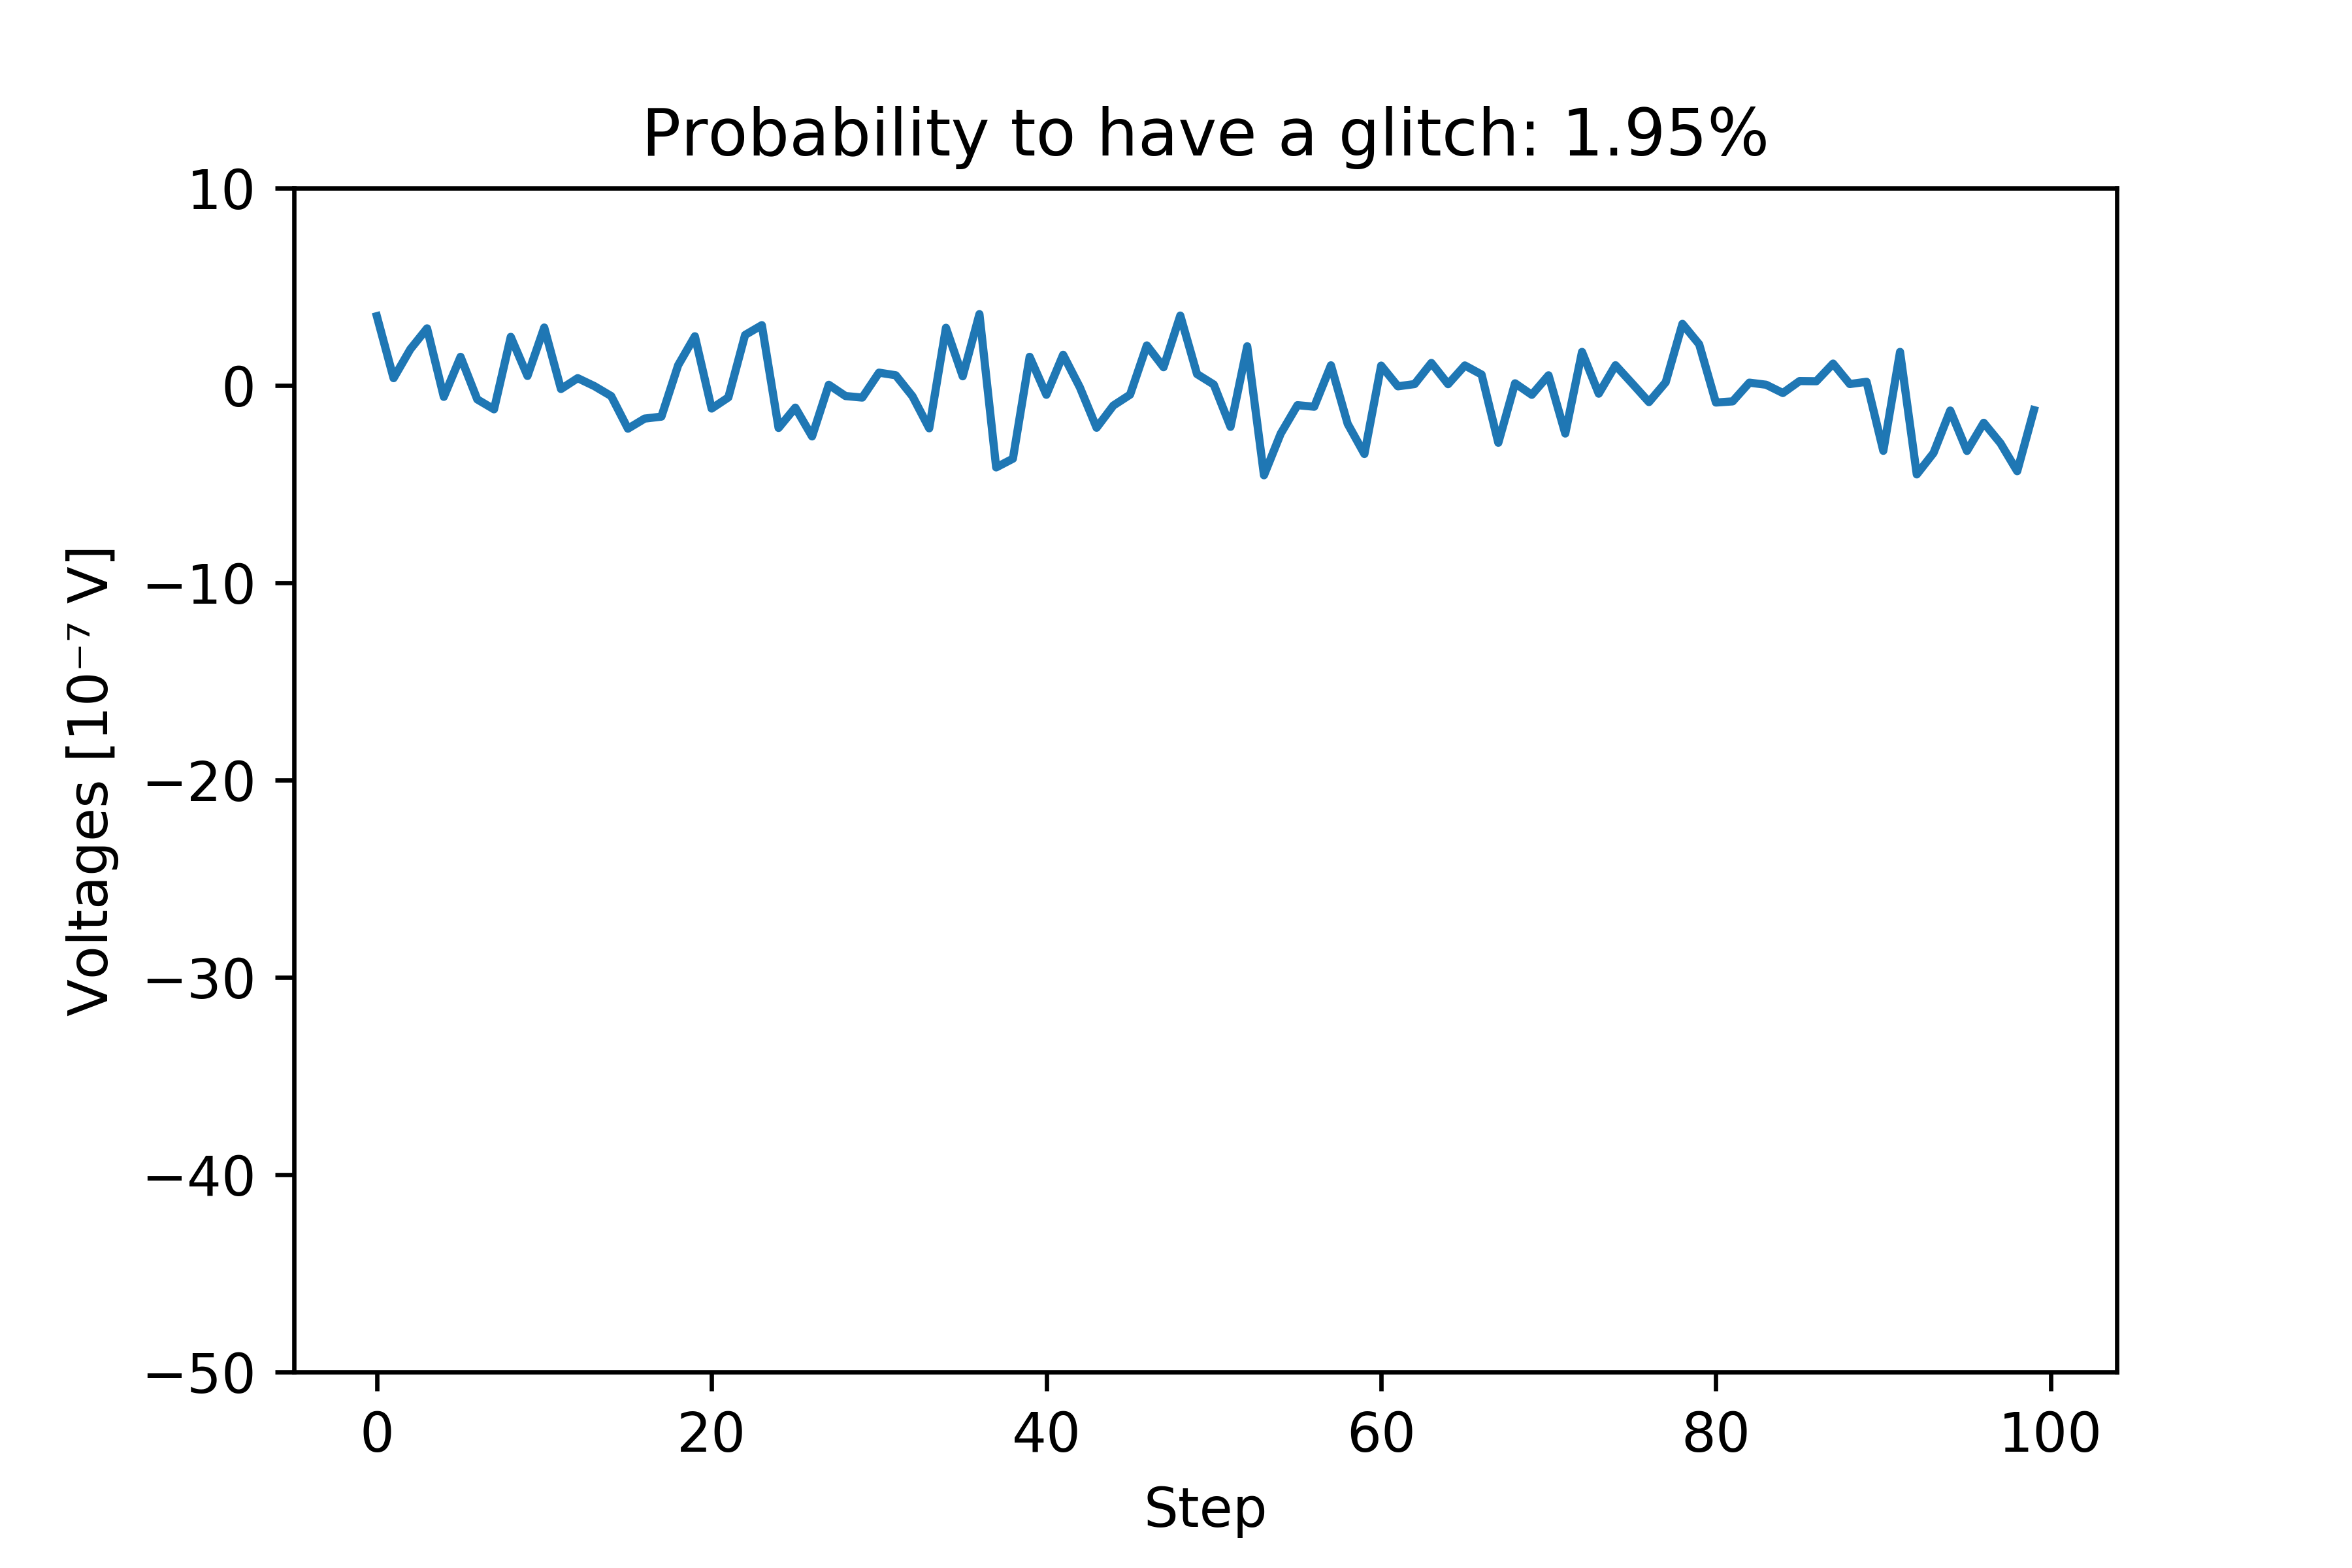
\includegraphics[scale=0.5]{test_plots/plot_1.png}
					\caption{}
				\end{subfigure}			
				\begin{subfigure}[t]{0.5\textwidth}
				
					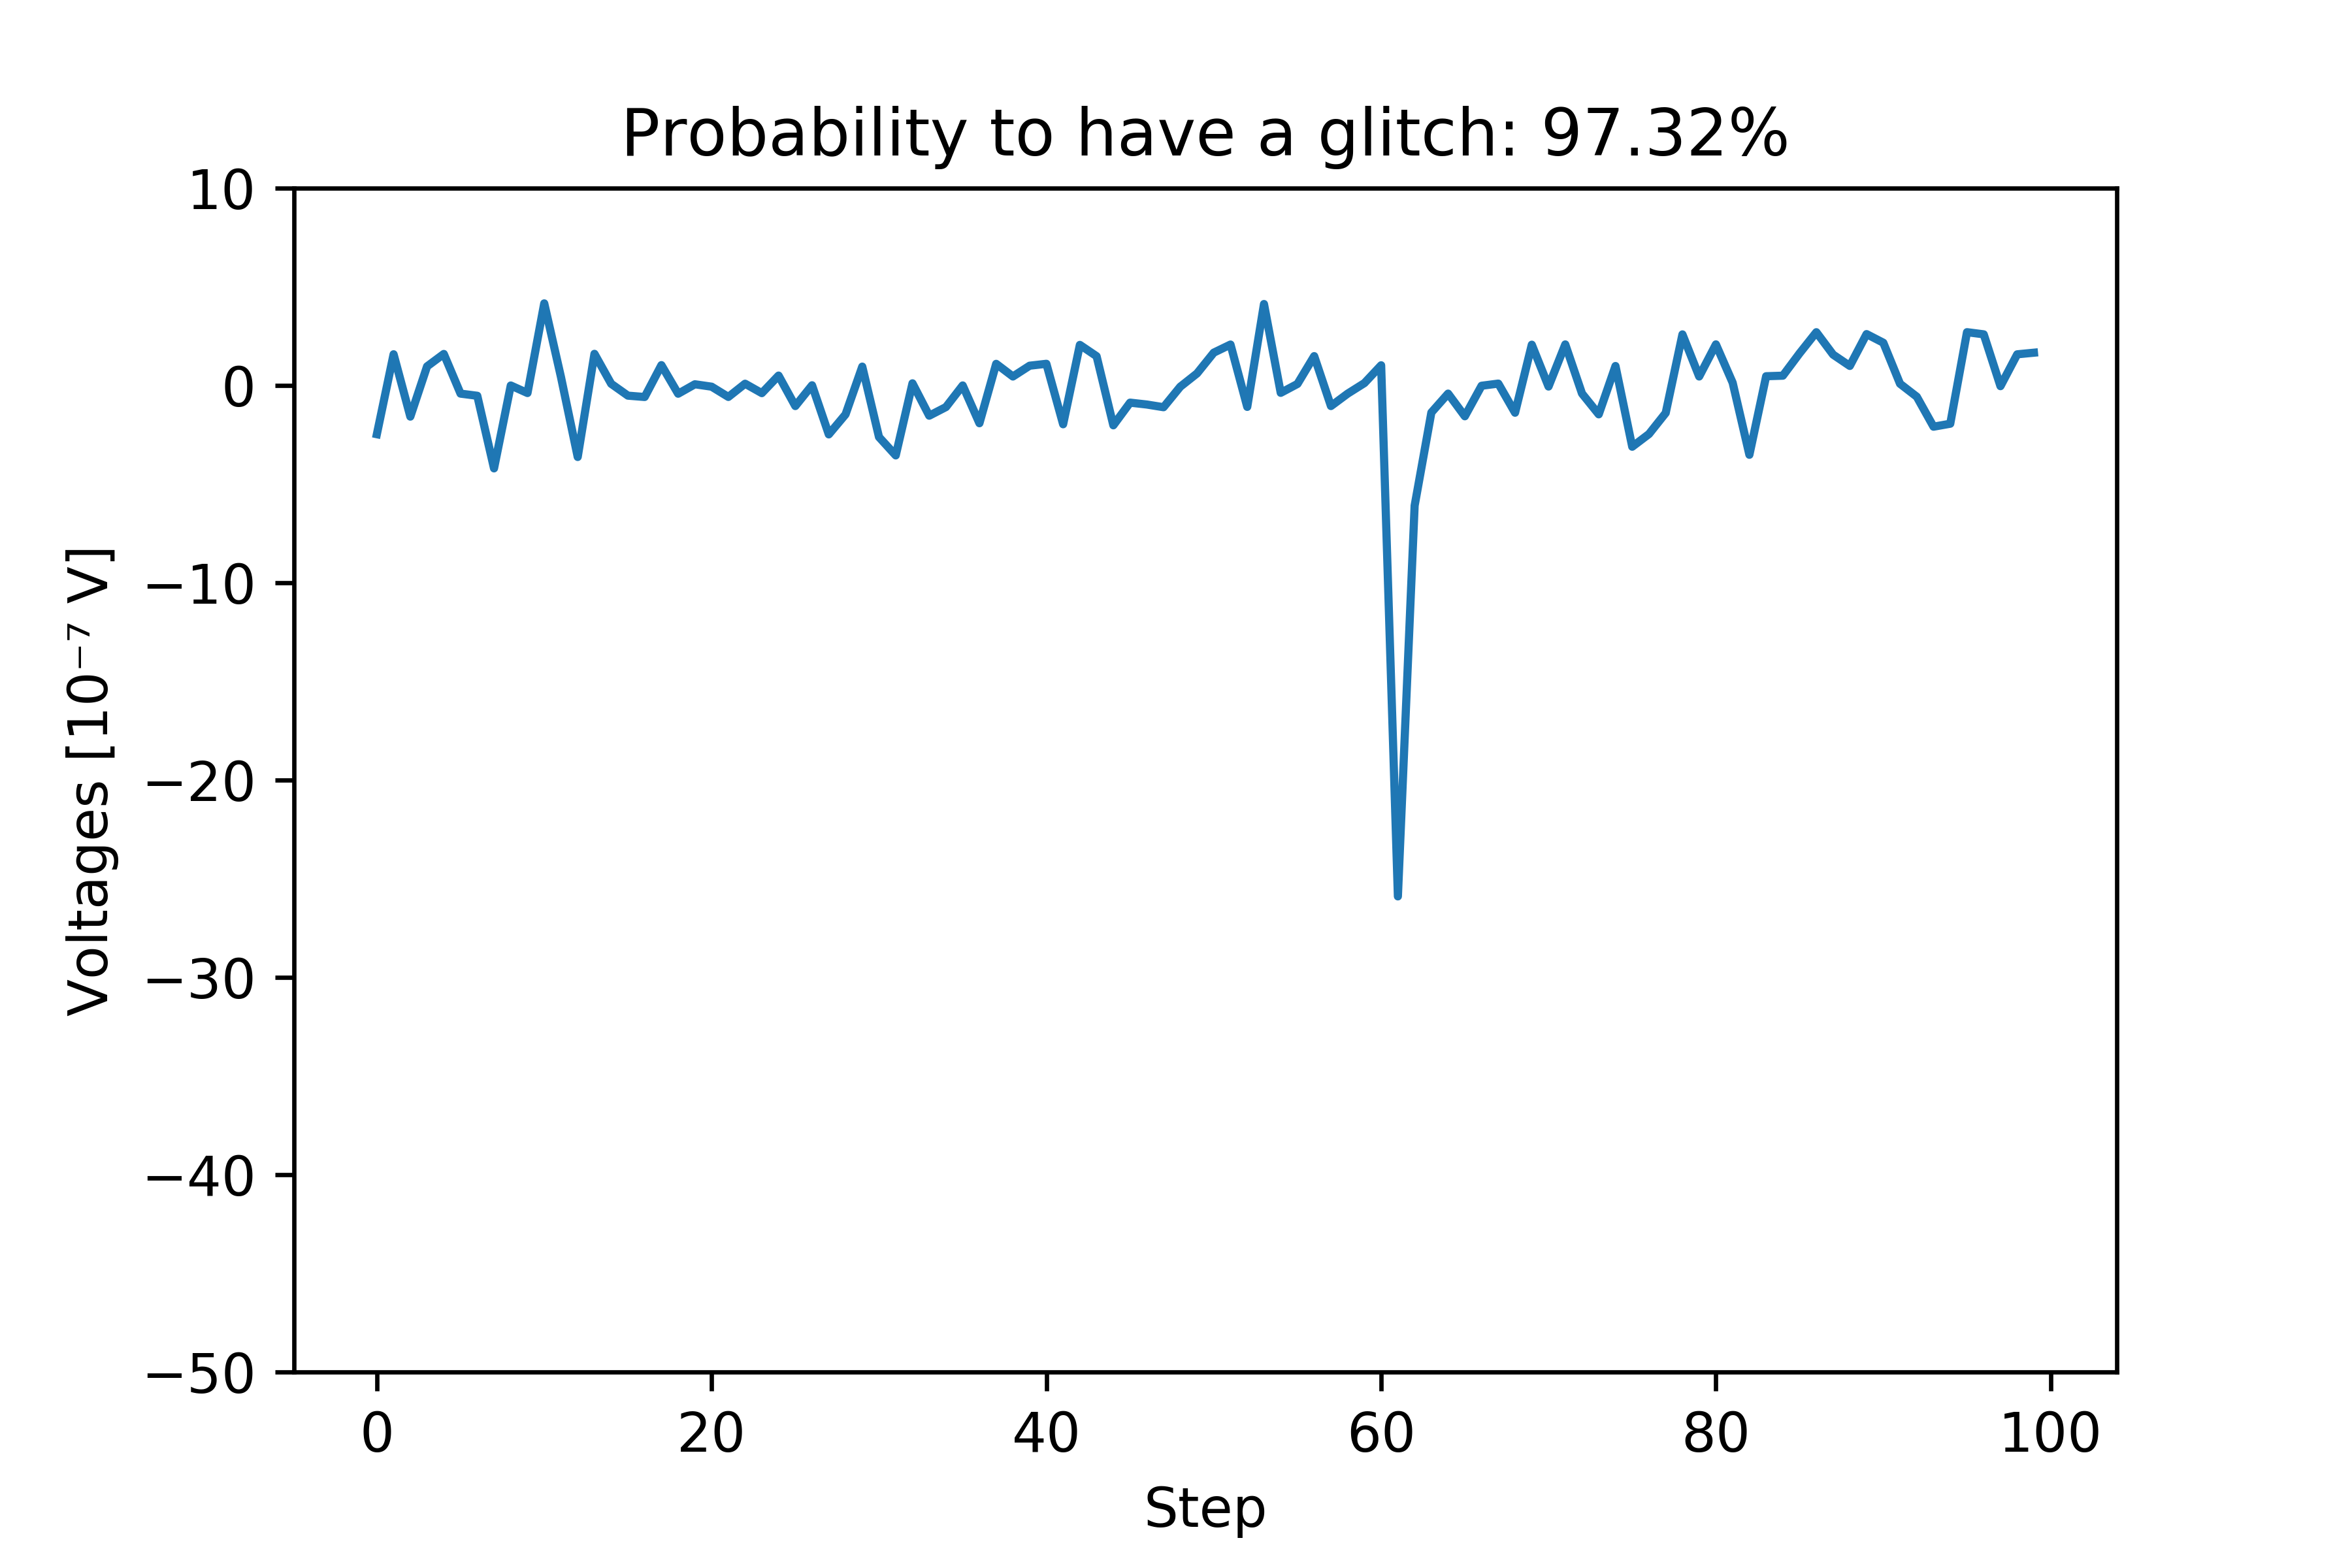
\includegraphics[scale=0.5]{test_plots/plot_10.png}
					\caption{}
				\end{subfigure}		
				
				  \captionsetup{singlelinecheck=off}
				\caption[]{Examples of a \textit{glitch} and a \textit{non-glitch} for the data pool:
					\begin{itemize}
						\item \texttt{Day: 94}
						\item \texttt{Frequency: 100$~\unit{GHz}$}
						\item \texttt{Bolometer: 1a}
					\end{itemize}
					The overall accuracy reached with this testing set is $98\%$.
					}
				\label{fig:test_plot_1}
			\end{figure}
			\smallskip
			%
			%
			%
			%
			\begin{figure}[h!]
				
				\begin{subfigure}[t]{0.5\textwidth}
				
					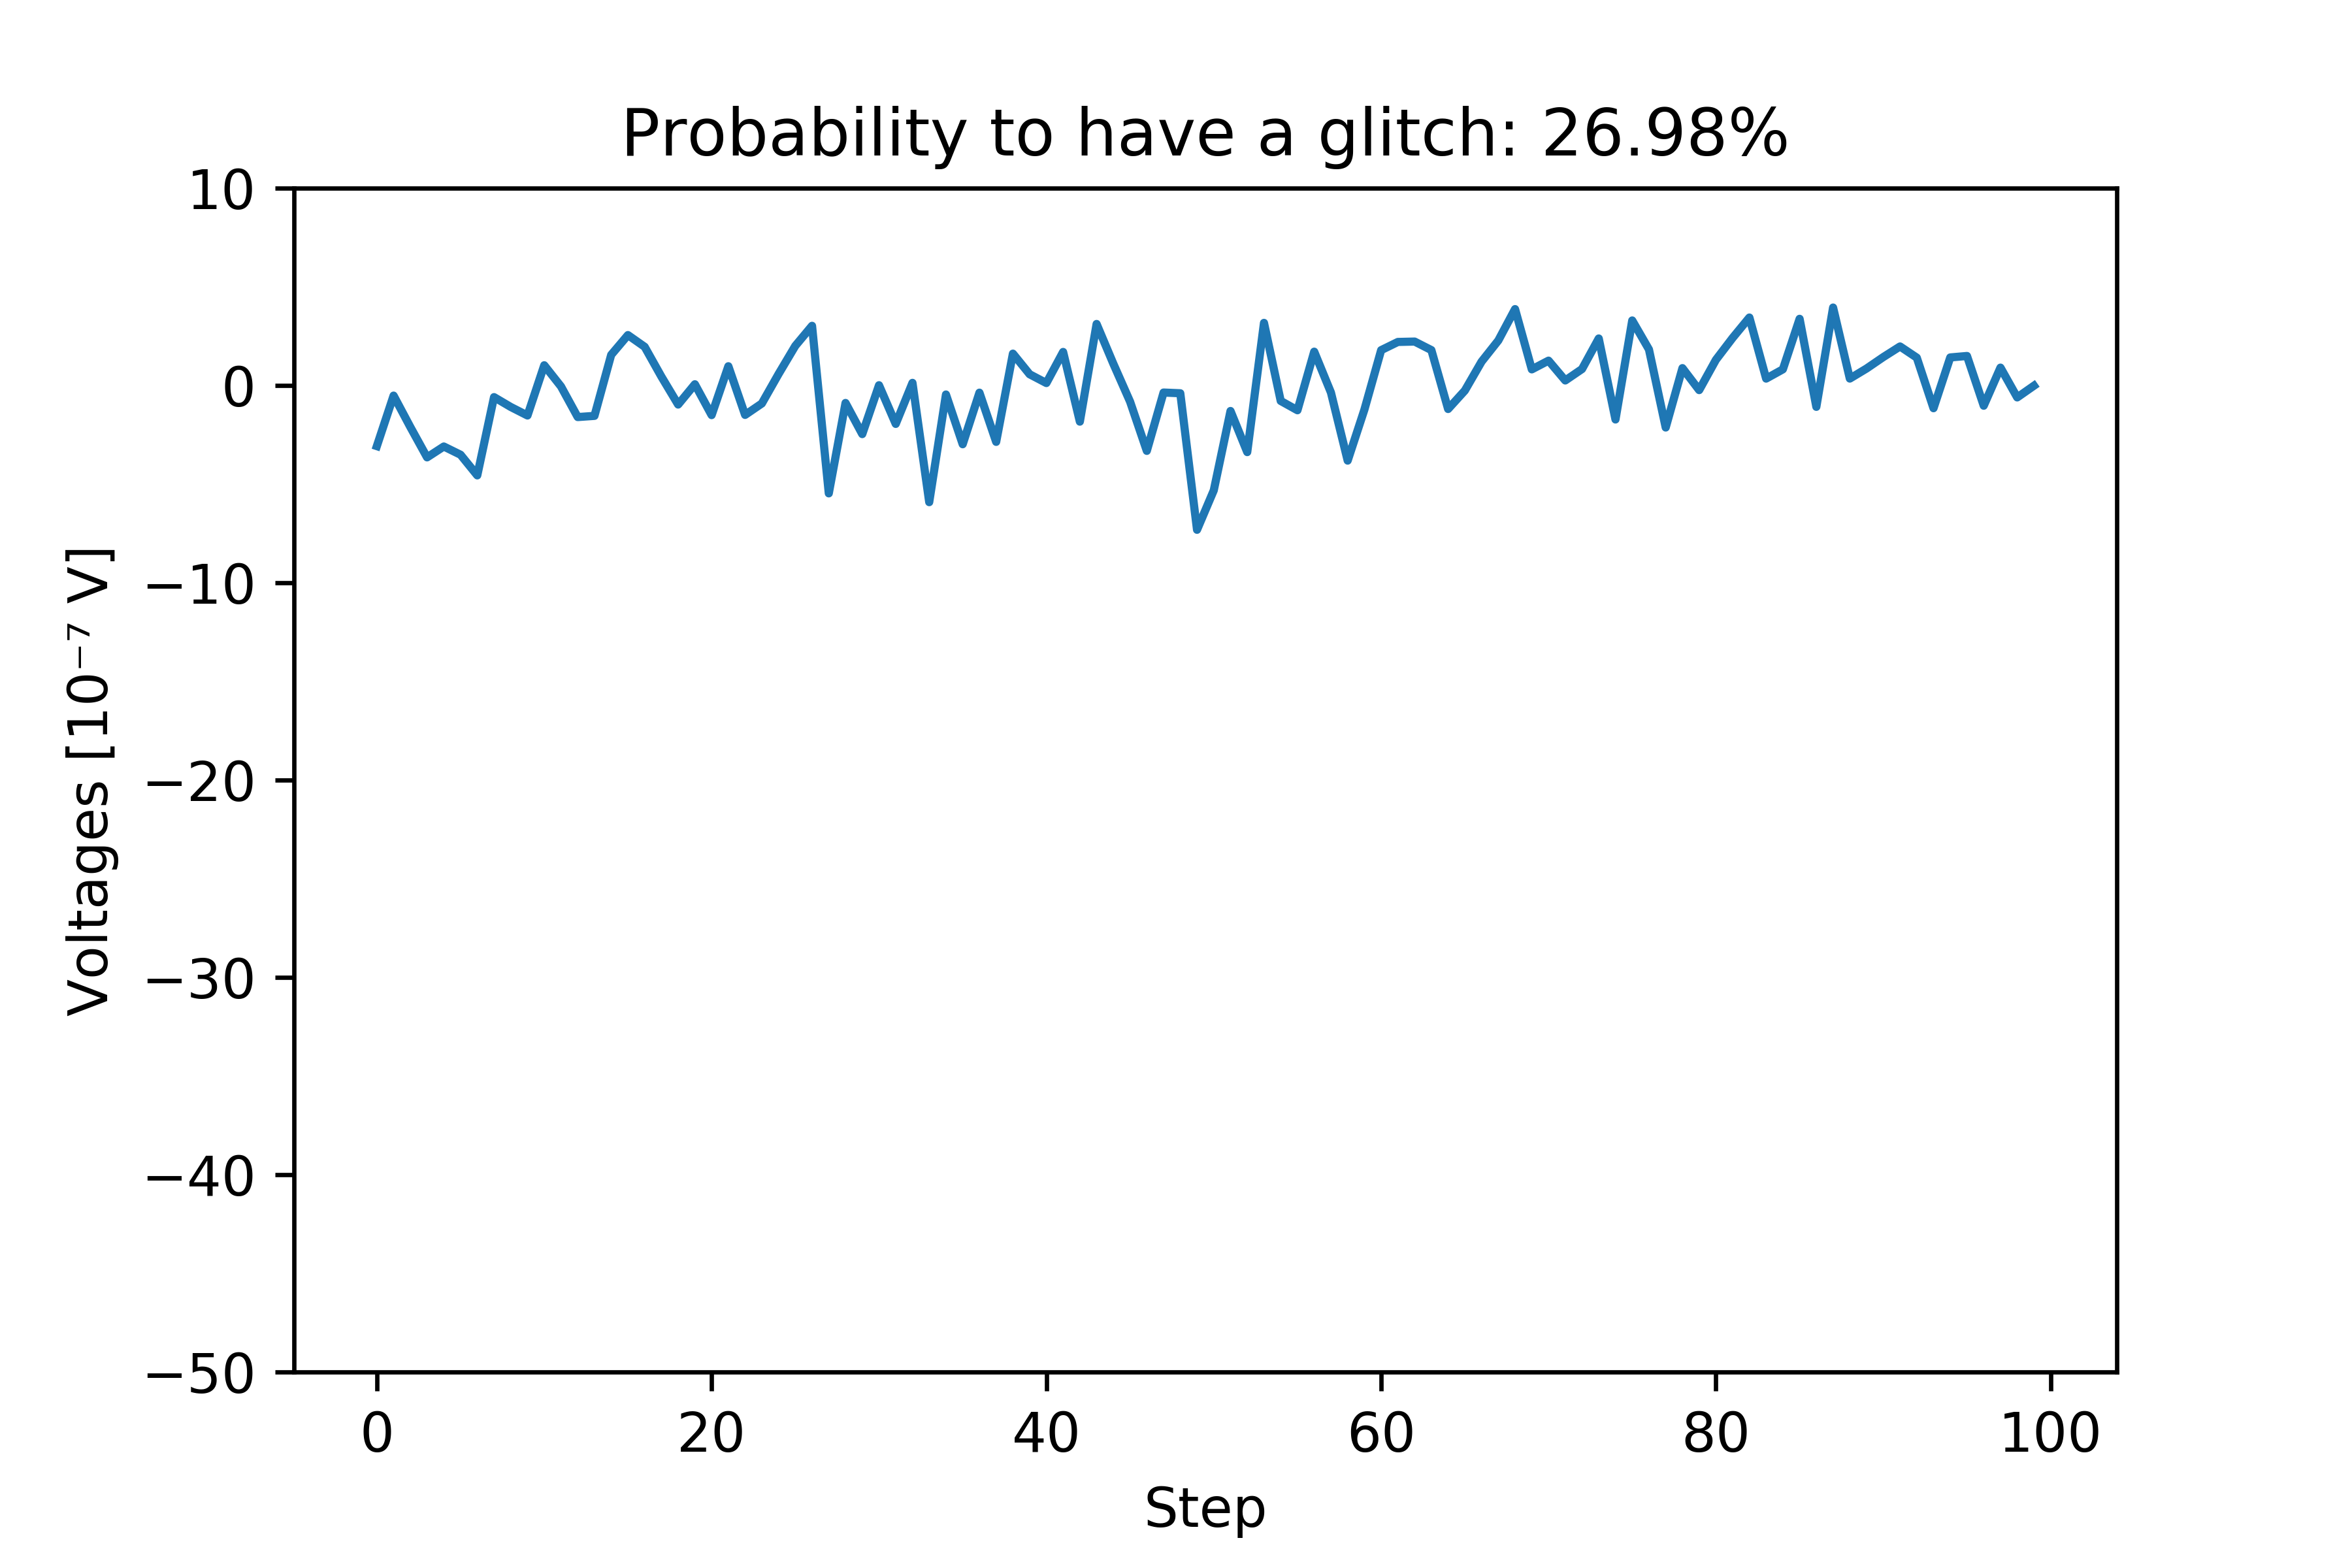
\includegraphics[scale=0.5]{test_plots/plot_1_2.png}
					\caption{}
				\end{subfigure}			
				\begin{subfigure}[t]{0.5\textwidth}
				
					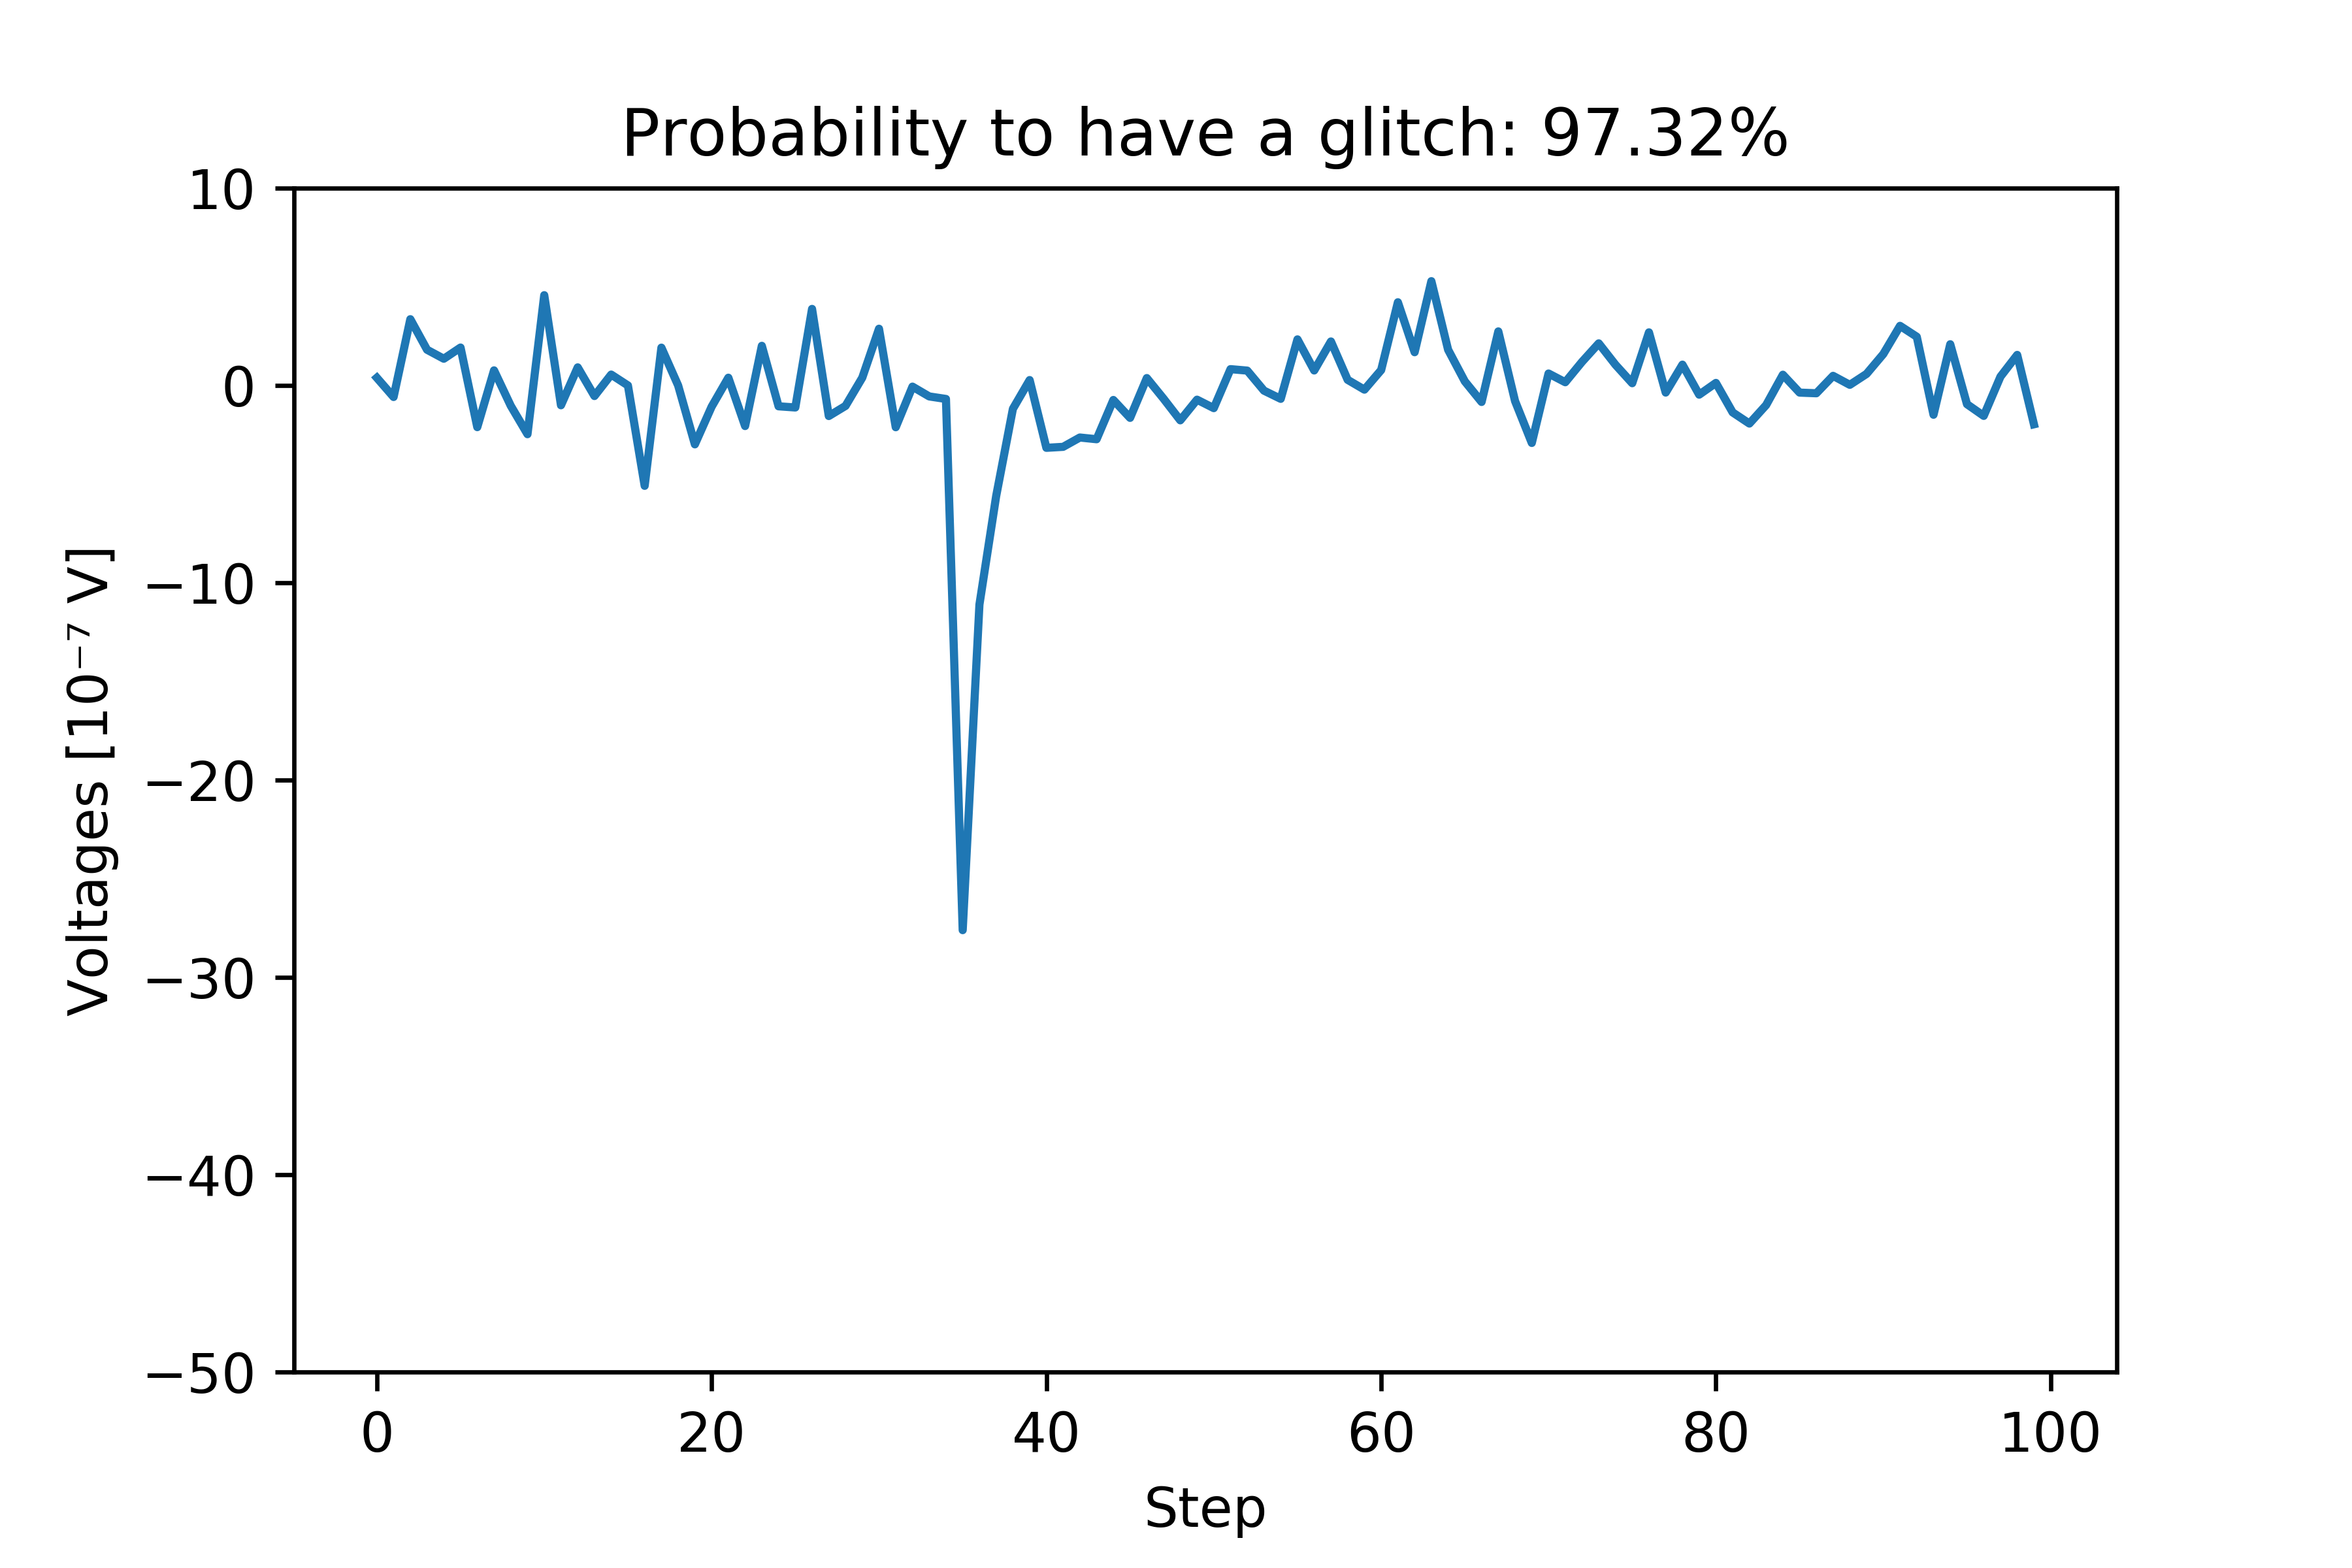
\includegraphics[scale=0.5]{test_plots/plot_7_2.png}
					\caption{}
				\end{subfigure}		
				
				  \captionsetup{singlelinecheck=off}
				\caption[]{Examples of a \textit{glitch} and a \textit{non-glitch} for the data pool:
					\begin{itemize}
						\item \texttt{Day: 100}
						\item \texttt{Frequency: 100$~\unit{GHz}$}
						\item \texttt{Bolometer: 2a}
					\end{itemize}
			The overall accuracy reached with this testing set is $99\%$.
					}
				\label{fig:test_plot_2}
			\end{figure}
			\smallskip
			%
			%
			%
			%
			\begin{figure}[h!]
				
				\begin{subfigure}[t]{0.5\textwidth}
				
					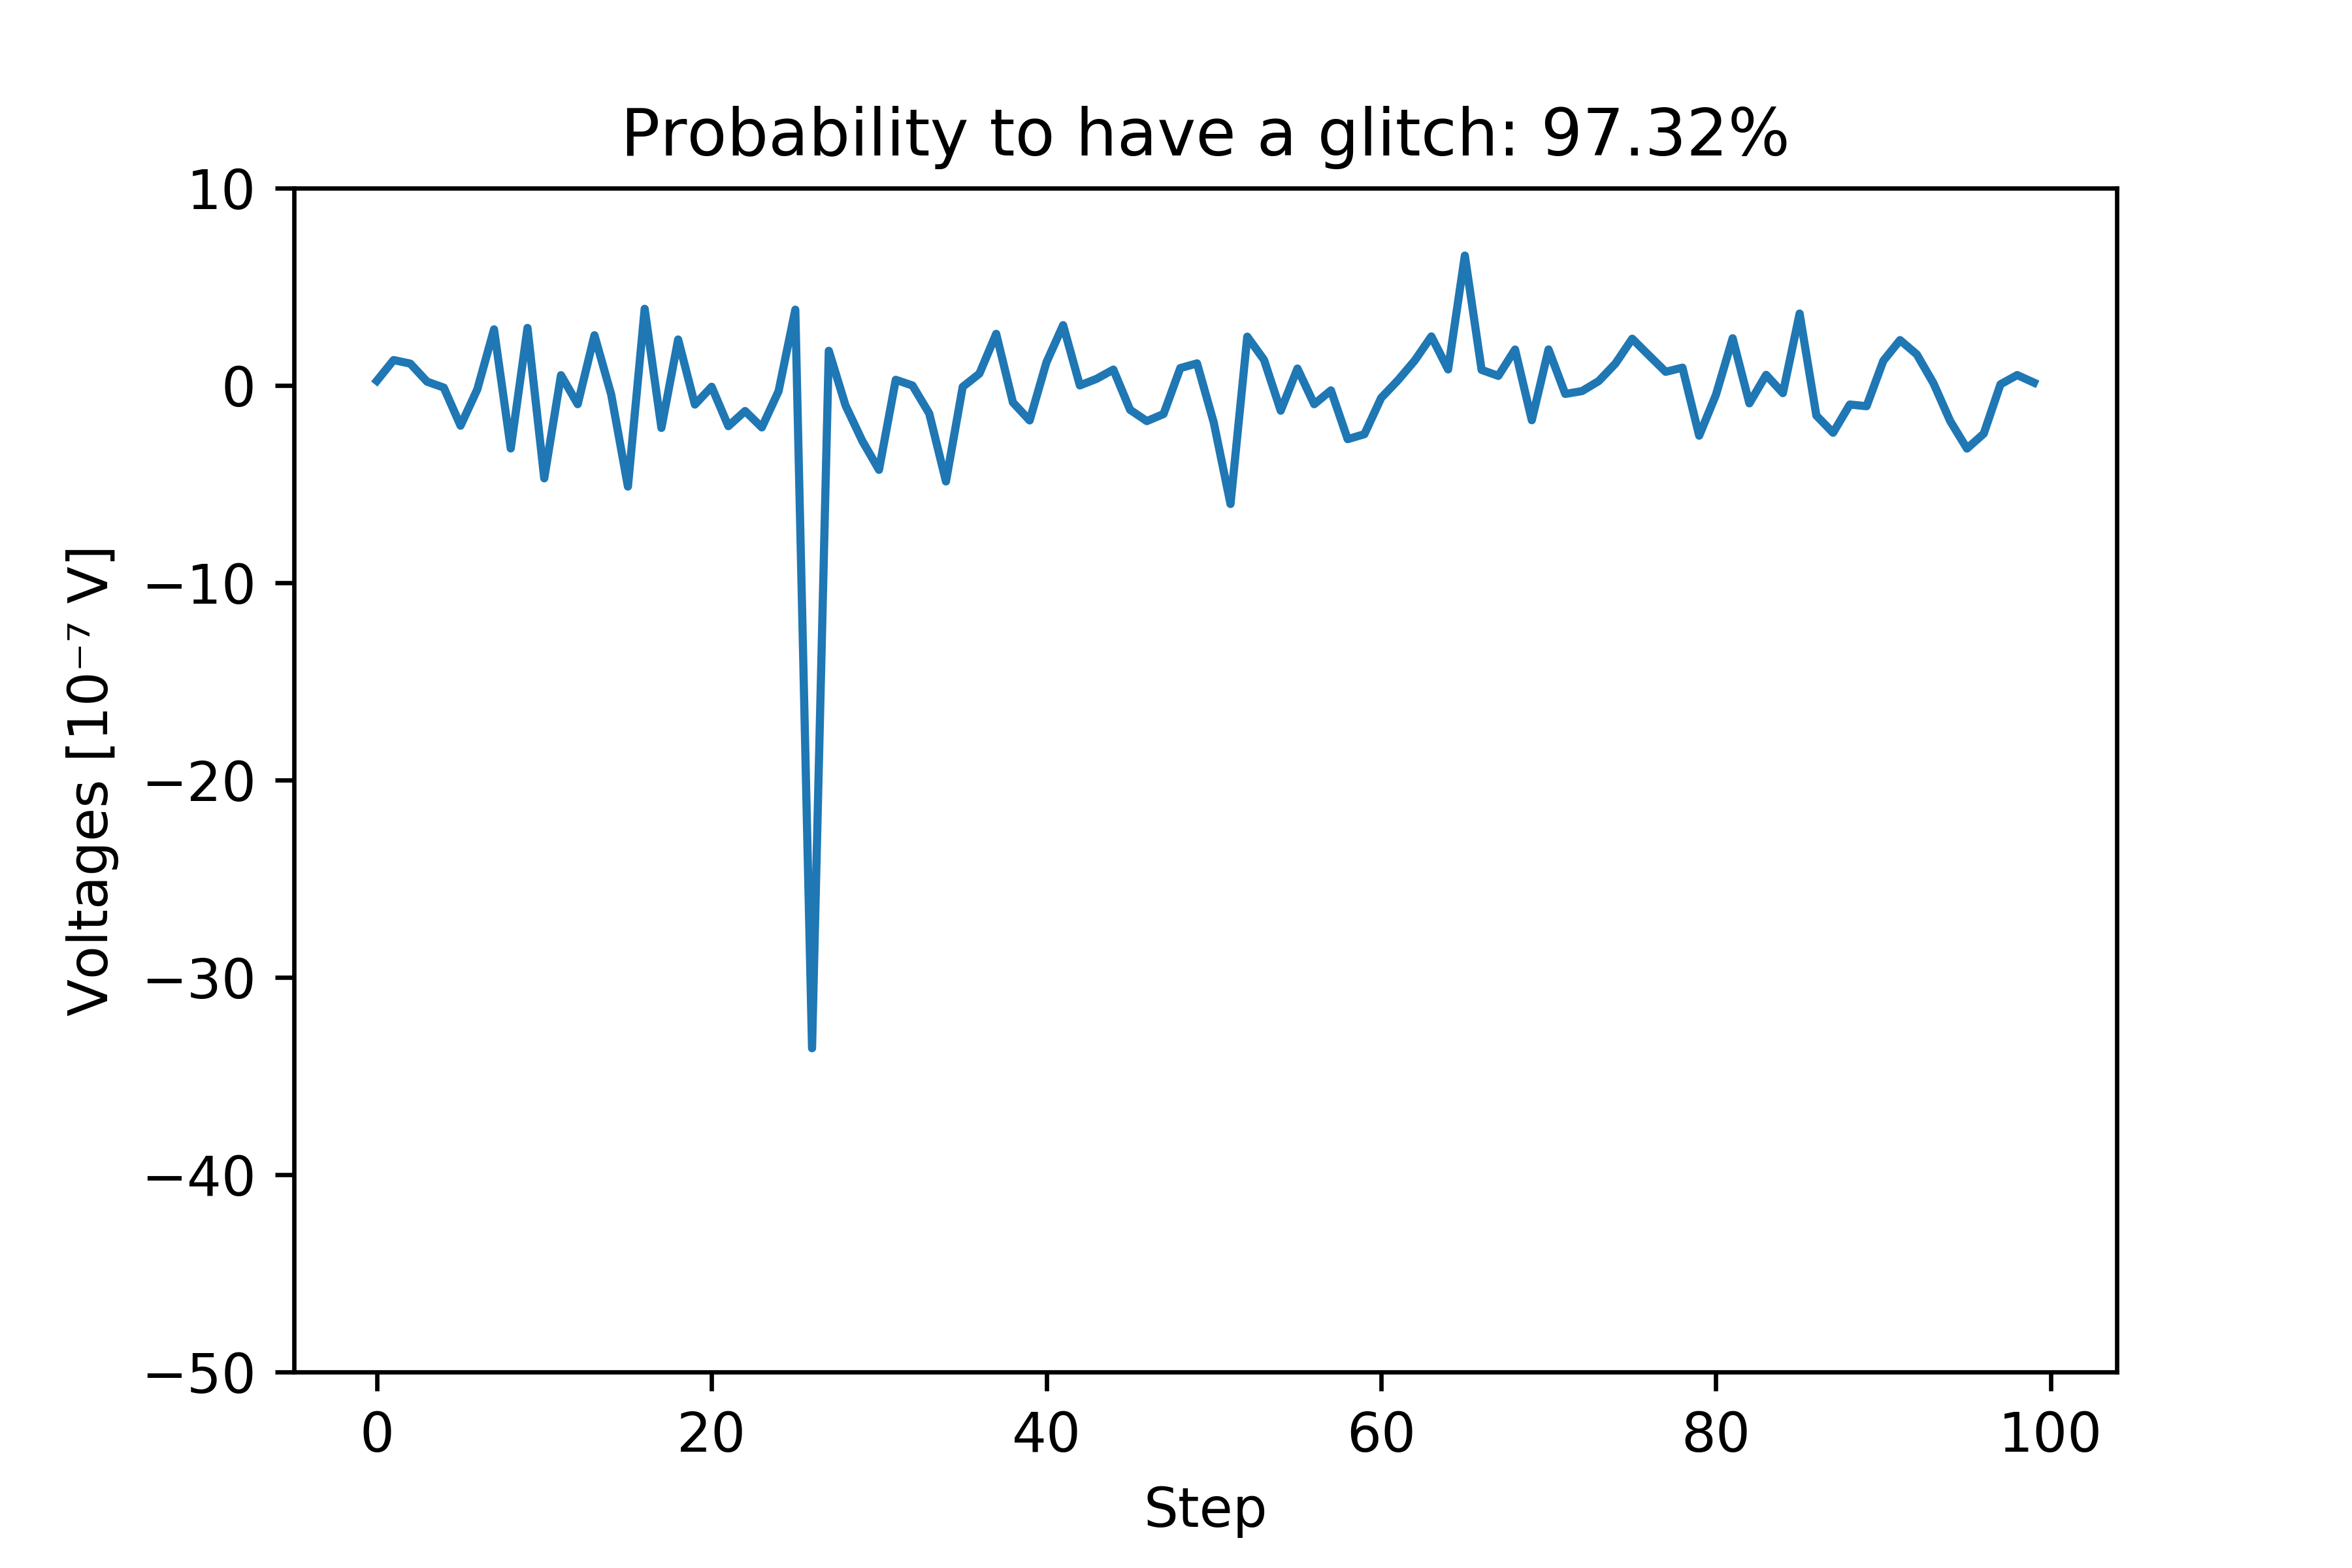
\includegraphics[scale=0.5]{test_plots/plot_5_3.png}
					\caption{}
				\end{subfigure}			
				\begin{subfigure}[t]{0.5\textwidth}
				
					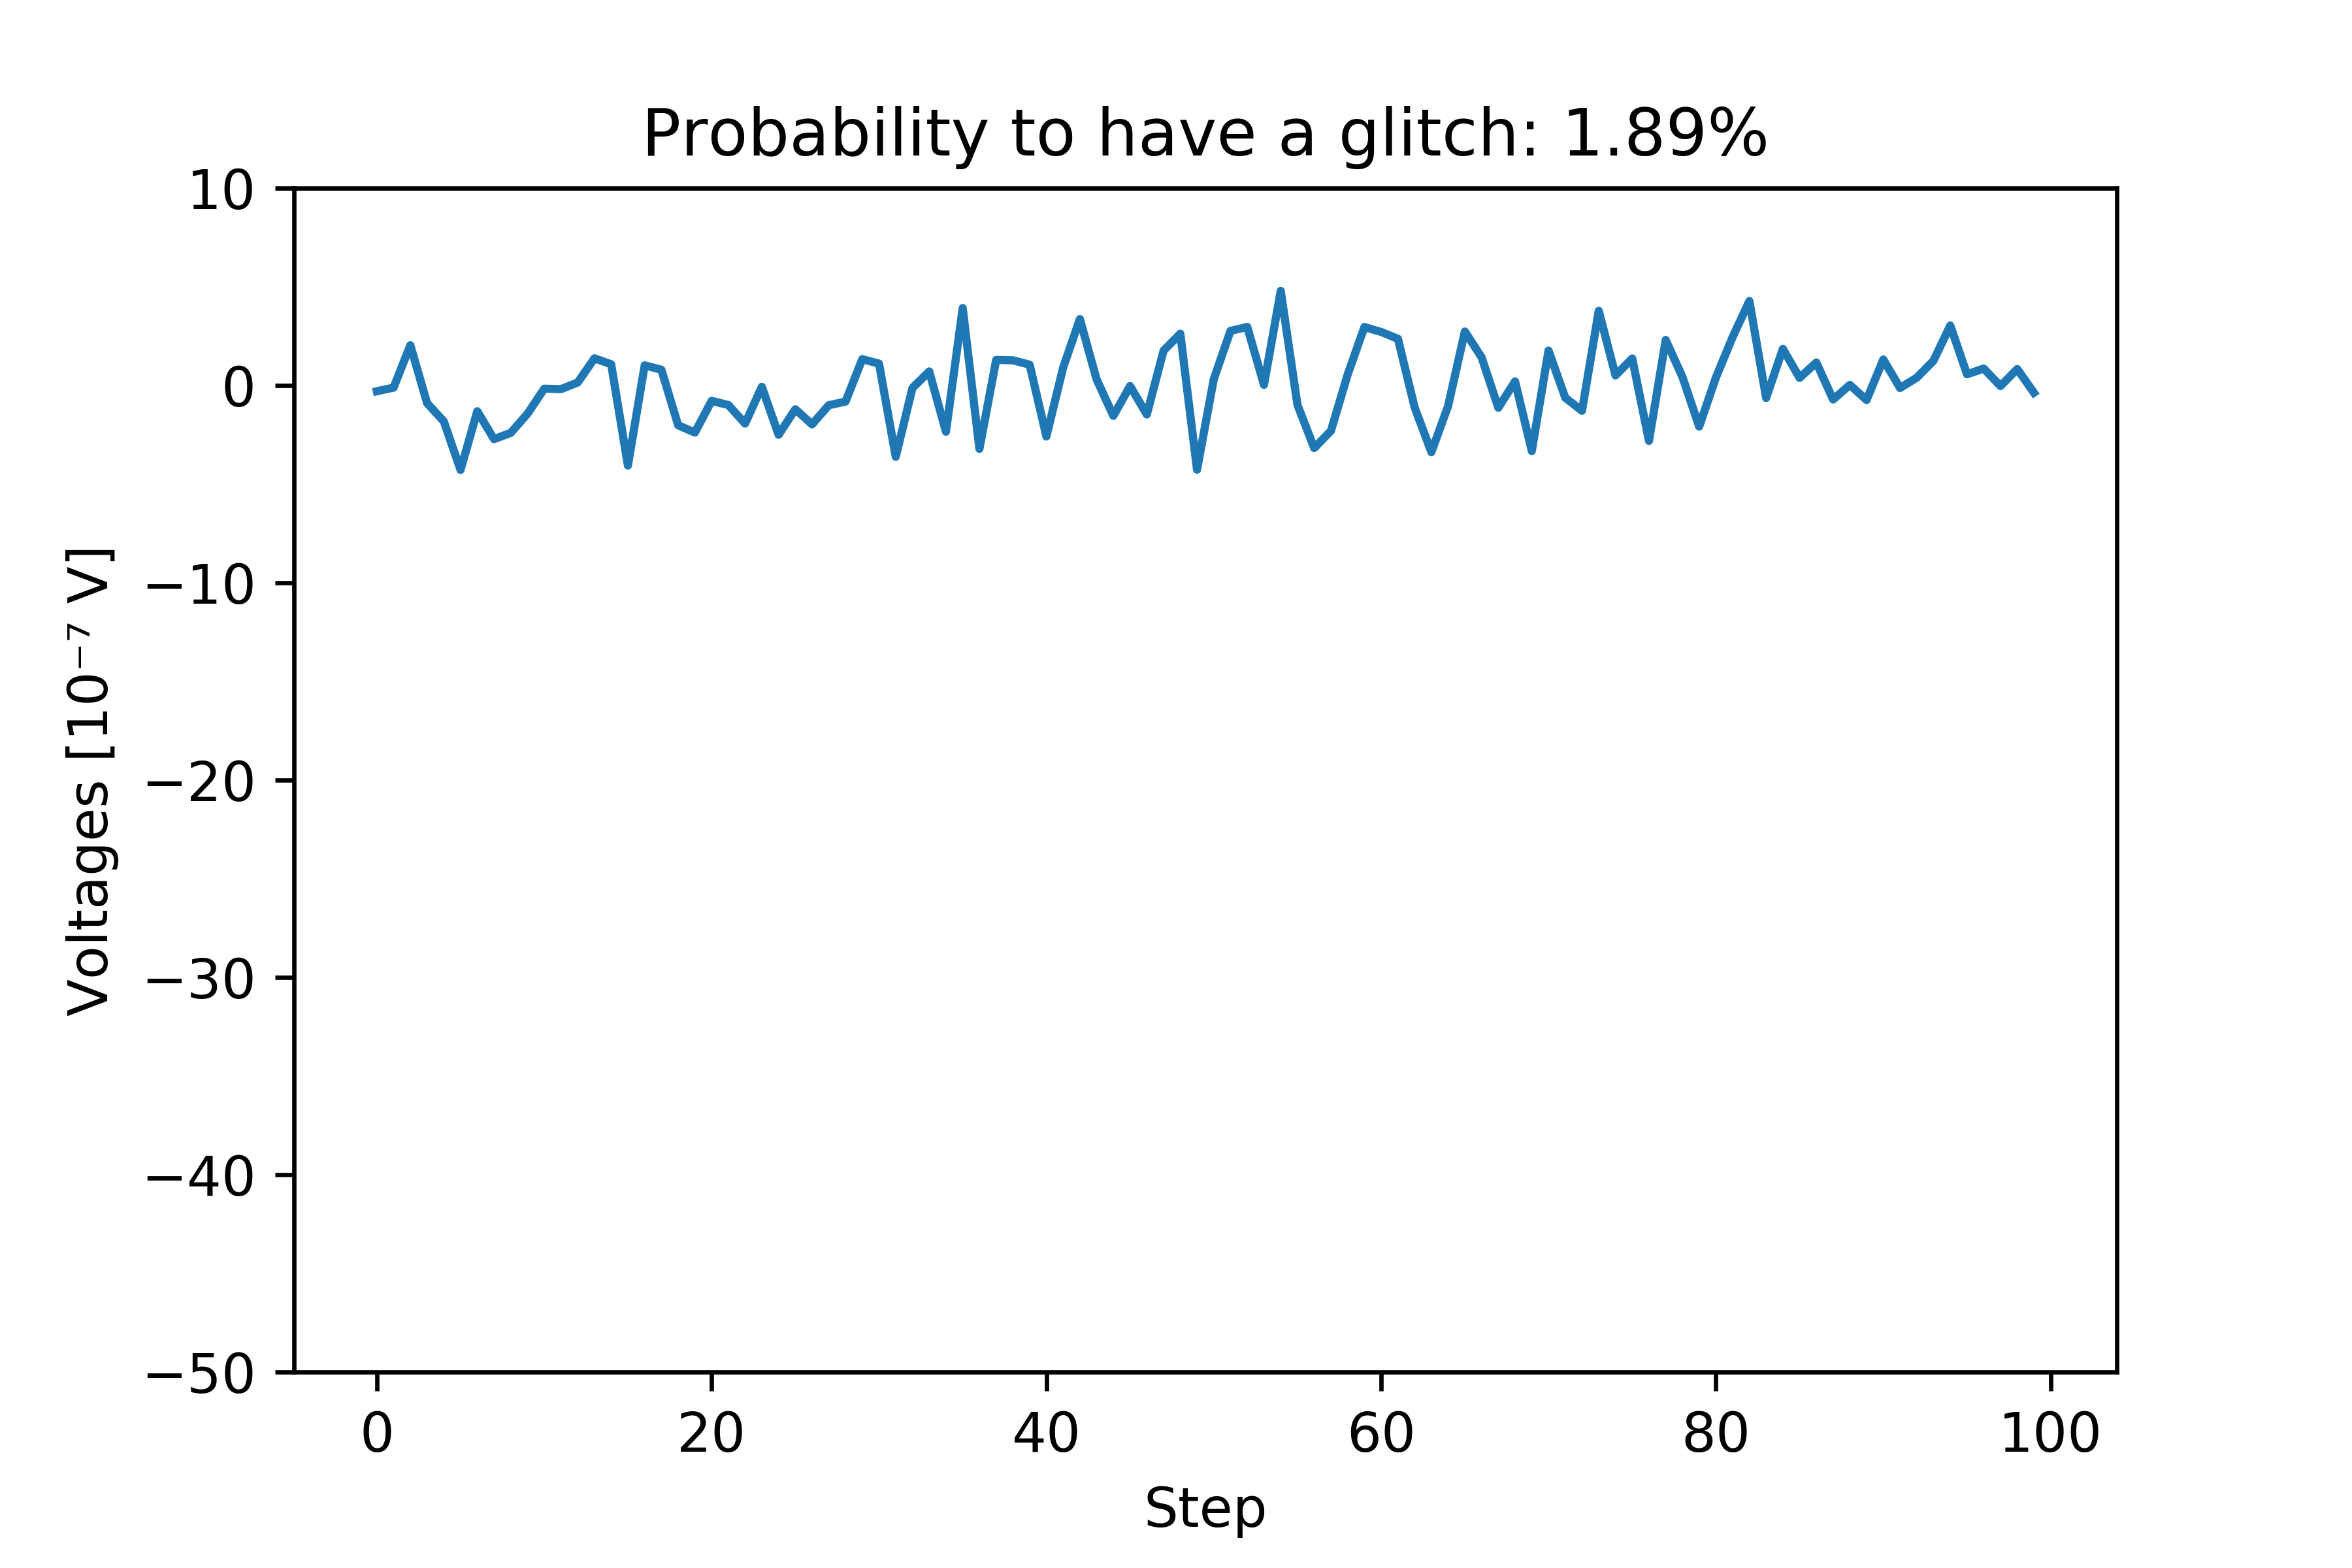
\includegraphics[scale=0.5]{test_plots/plot_7_3.png}
					\caption{}
				\end{subfigure}		
				
				  \captionsetup{singlelinecheck=off}
				\caption[]{Examples of a \textit{glitch} and a \textit{non-glitch} for the data pool:
					\begin{itemize}
						\item \texttt{Day: 104}
						\item \texttt{Frequency: 143$~\unit{GHz}$}
						\item \texttt{Bolometer: 1a}
					\end{itemize}
				The overall accuracy reached with this testing set is $97\%$.
					}
				\label{fig:test_plot_3}
			\end{figure}
			%
			%
			%
			\clearpage
			\subsection{Classifier with RMS}\label{classifier_with_rms}
			As a final test, I classified 100 new timeseries from the initial set of data (day $93$ for the bolometer \texttt{1a} at $100~\unit{GHz}$) and tested it compared to a simple RMS classifier made by me.			
			
			The RMS classifier's role is to compare my model with one similar to what the \textit{HFI} team used in their data-analysis pipeline. Unfortunately, I had no access to the aforementioned pipeline, so, in order to compare how the collaboration managed to clean glitches present in the data, I had to build something by myself. \cite{planck_glitches}
			I divided each timeseries (100 steps) into $7$\footnote{This number was chosen using a simple optimization: it was the one that gave the best results.} blocks, evaluate the quadratic mean (RMS) for each block and then consider the largest of these values; I shall call this number \texttt{rms\_max} for convenience. Fig. \ref{rms_max_plot} shows the calculated values on the 100 testing timeseries, classified as in Section \ref{data_classification}. 
			\begin{figure}[h!]
			\centering
				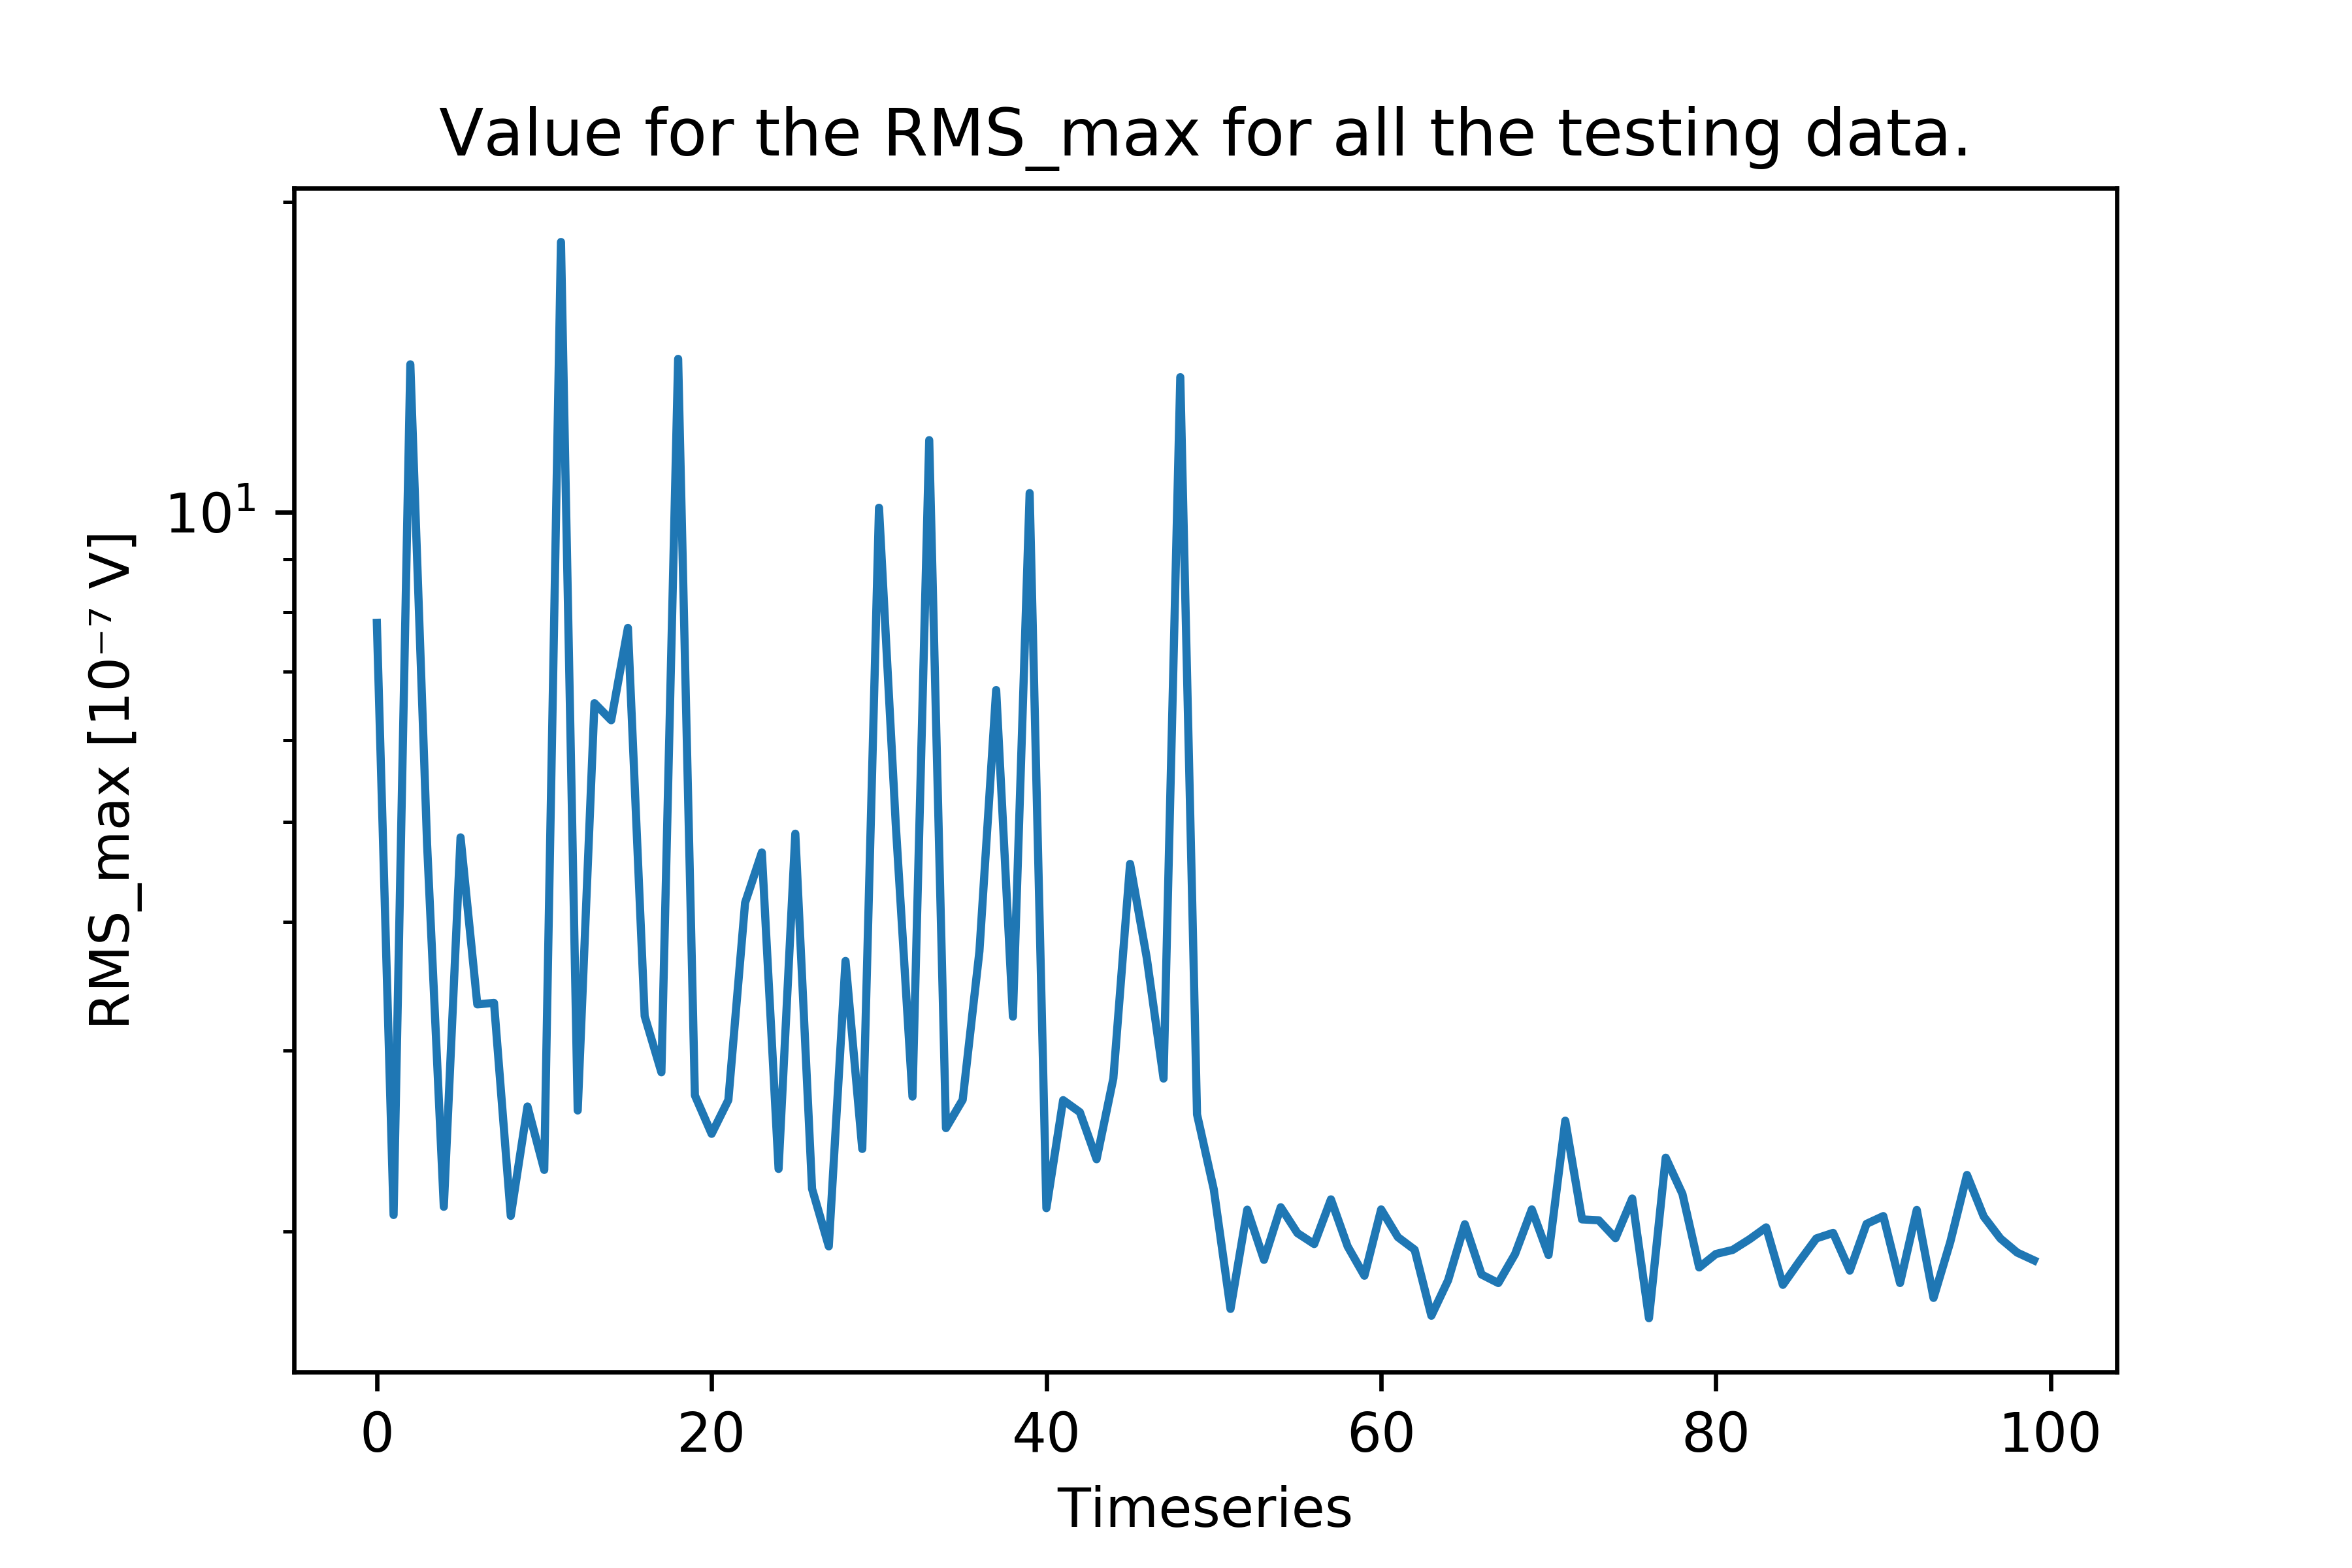
\includegraphics[scale=0.65]{figures/rms_max.png}
				\caption{\texttt{rms\_max} for each of the $100$ timeseries. The first $50$ are batches that present a \textit{glitch}, while the last $50$ are without it.	\\
				I used a logarithmic scale to enhance the values, due to the fact that some of the timeseries with \textit{glitch} present a very high value for the \texttt{rms\_max}.}
				\label{rms_max_plot} 
			\end{figure}
			
			I picked a \textit{threshold}, i.e. a  value for the \texttt{rms\_max} which would discriminate between \textit{glitch} and \textit{non-glitch}. As \textit{threshold}, I took the lowest \texttt{rms\_max} that resulted from the batches classified as \textit{glitch}. 
			Using this methodology, the accuracy I managed to get was:
			\begin{center}
				\texttt{accuracy\_rms = 97\%}
			\end{center}
			This technique is by far more effective than using the total RMS for each timeseries: with the latter, the best accuracy I managed to get did not go above $90\%$.
			
			In the next Section, I present the results obtained on the same data using \textit{Neural Network}.
			
			\subsection{Results with test data}
			% Aggiungi grafici di casi in cui il network ci ha azzeccato mentre io ho sbagliato completamente.
				Using the same data pool as in the previous Section, hence $100$ timeseries from the initial data set, I set out to establish how the network, as trained, would work. It is important to note that, in this testing data set, I tried to avoid uncertain cases, and instead I decided to use only timeseries where the classification would be obvious. 
				A simple evaluation gave a perfect $100\%$ result, which gives the information that, in cases where there is no reasonable doubt about the classification, the network works perfectly. This highlights how, compared to a simple RMS program, as the one in Section \ref{classifier_with_rms}, it yields better results (a $3\%$ increase in my data set).				
				
					\begin{figure}[h!]
				\captionsetup{singlelinecheck=off}
				\centering
					\includegraphics[scale=0.8]{figures/confusion_matrix.png}
					\caption[foo bar]{Confusion matrix for the test data with a threshold of $50\%$. Many configurations for this type of matrix can be chosen; the one I worked with is:
					\begin{itemize}
						\item In the upper left are the \textit{non-glitches} classified correctly.
						\item Upper right are the \textit{non-glitches} classified incorrectly (hence as glitches).
						\item In the bottom left are the \textit{glitches} classified incorrectly as \textit{non-glitches}.
						\item Bottom right are the \textit{glitches} classified correctly.
					\end{itemize}
					}
					\label{fig:confusion_matrix}
				\end{figure}		
				
				In order to show how good the network can actually perform, a simple evaluation is not sufficient. Indeed, when one undergoes a testing of a network, it must bear in mind that what the network gives as output are just probabilities. This leaves the task to decide a \textit{threshold} for said probabilities.
				Let us call this new threshold \texttt{test\_threshold}. Let us consider as an example the situation in which one chooses \texttt{test\_threshold = $20\%$}. In this case, all of the timeseries for which the network outputs a probability higher than $20\%$ will be labeled \textit{glitch}, while those with probability lower will be labeled \textit{non-glitch}.
				In the evaluation above, a general threshold of $50\%$ was chosen; but different values could be used to yield different results. In order to see how actually a network performs, one must test it for different thresholds.						
				
					The best way to evaluate the performance of a network under different thresholds is by means of a \textit{Confusion Matrix}. The confusion matrix has in it, for a given threshold, the amount of data that is correctly and incorrectly classified, discriminating between \textit{glitch - correct/incorrect} and \textit{non-glitch - correct/incorrect}. 
				In Fig. \ref{fig:confusion_matrix} is an example for the confusion matrix with the testing data for a \texttt{test\_threshold = 50\%}. As one can see, all of the data is correctly classified using said configuration.
				
				To see how the network performs under a different set of thresholds, one can draw a plot: the \textit{ROC curve}. The \textit{ROC}'s role is to show how the confusion matrix's results change with a changing threshold; more specifically, it plots the \textit{false positive rate} (how many \textit{non-glitches} are classified as \textit{glitches}) to the \textit{true positive rate}, which are both directly dependent on the threshold.
				Defined like this, the values I would \textit{expect} are as follow:
				\begin{itemize}
					\item For a low threshold, $100\%$ for the \textit{true positives} and a non zero value for the \textit{false positives}. When \texttt{test\_threshold = 0\%}, both values should be at $1$.
					\item For a high threshold, the \textit{true positives} should still be more than the \textit{false positives}, but they could both have values lower than $100\%$. When one has \texttt{test\_threshold = 100\%}, both of the variables should go to $0$.
				\end{itemize}
					The best results that can be obtained from a testing pool of data is an ``upside down L". When this occurs, it implies a high confidence in the network's predictions, even though it is never perfectly either $0\%$ or $100\%$.
				Fig. \ref{fig:roc_curve} shows the \textit{ROC curve} obtained with the already mentioned testing data. It is easy to see that, even if obtained using a high number of points, it is a perfect "upside down L", which means that, for this testing data, the network is almost perfect.
				\begin{figure}[h!]
				\centering
					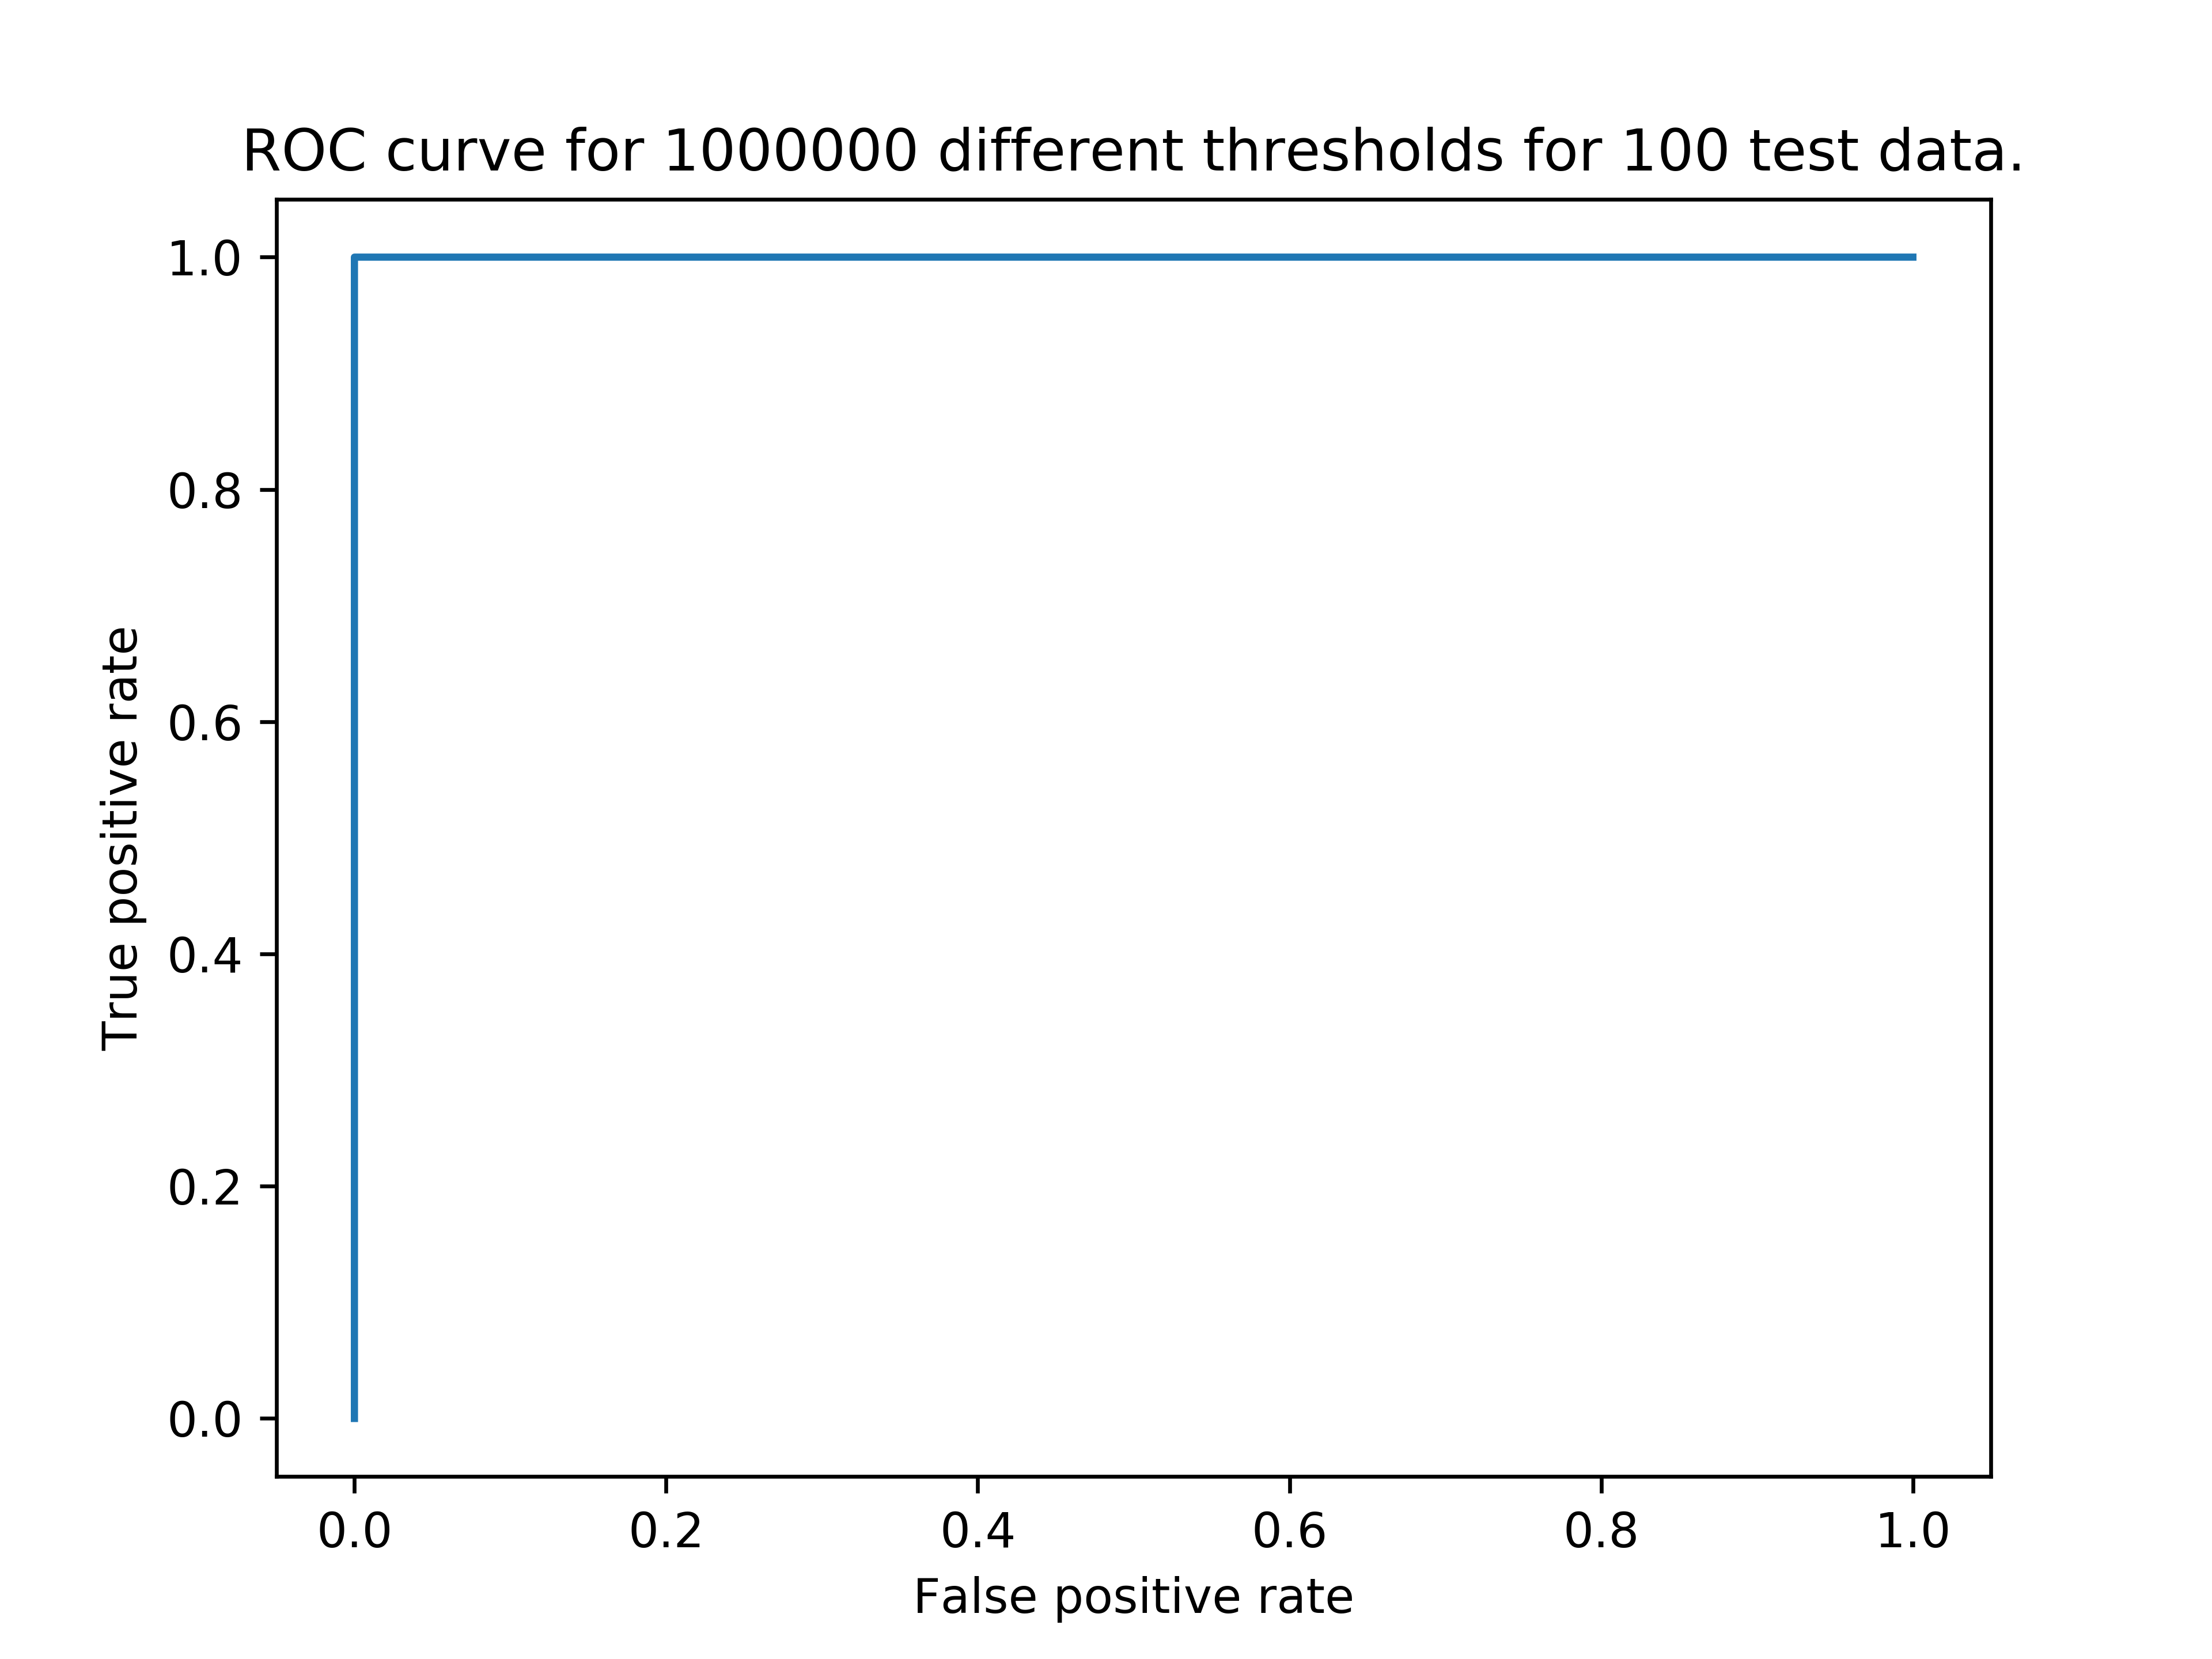
\includegraphics[scale=0.8]{figures/ROC.png}
					\caption{ROC curve for the test data evaluated on $1$ million different thresholds. For my network, the results are almost perfect, even though the points are evenly distributed along the curve (they could not be plotted due to the large number of them.}
					\label{fig:roc_curve}
				\end{figure}							
					 
				If one wants to see a more tangible result, it is possible to calculate the area under the \textit{ROC curve}. What I obtained is a perfect:
				\begin{center}
					\texttt{ROC area = 1.0}
				\end{center}
				Which again, is a meter to establish how my network works seemingly perfect with the given testing data.				
				
				Even if the results are remarkable, it is important to remember that they were obtained using testing data from the same pool (day, frequency and bolometer) as the one used for both training and validation. 
				In this testing, I preferred to operate as shown, hence using testing data only from the same pool, to demonstrate how, if trained with a certain configuration, the results yielded are remarkable. In a real world application, one might expect to use training data from a much larger set of data (mostly different frequencies and bolometers) and, thus, hopefully get the same results as the one I have obtained but on a much broader scale.				 
				
				In Fig. \ref{fig:multi_roc} are the ROC curves and their area relative to the data in Fig.s \ref{fig:test_plot_1}, \ref{fig:test_plot_2} and \ref{fig:test_plot_3}. These results are not always as nearly perfect as in the main test described above, but the overall shape of all 3 shows a remarkable result. 				
				
				\begin{figure}[h!]
				\centering
					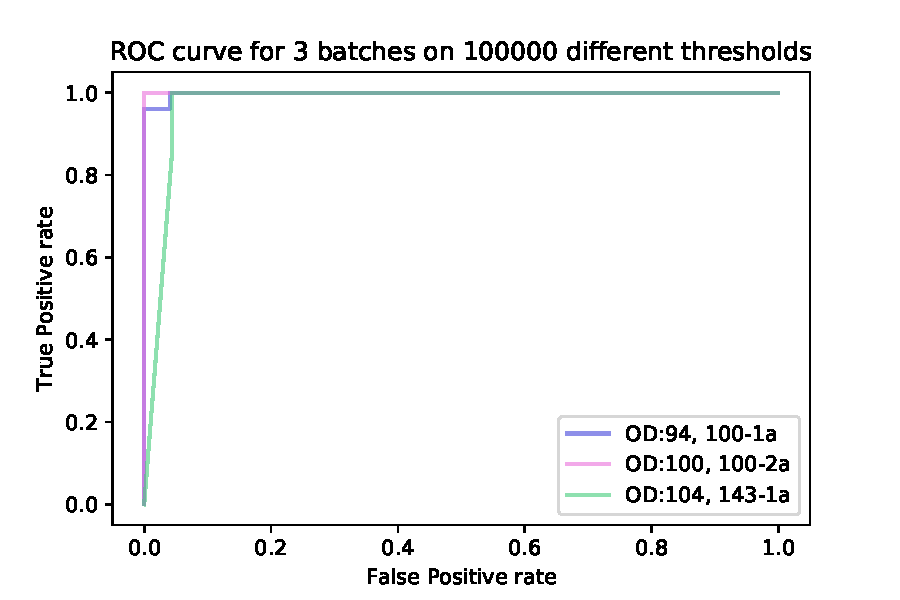
\includegraphics[scale=0.75]{figures/roc_best.pdf}
					\caption{ROC curves for the same data as in Fig.s \ref{fig:test_plot_1}, \ref{fig:test_plot_2} and \ref{fig:test_plot_3}. It represents, just like in the main test pool, correct positives to wrong negatives.}
					\label{fig:multi_roc}
				\end{figure}
%				\begin{figure}[h!]
%				\centering
%					\begin{subfigure}[t]{0.6\textwidth}
%									\centering
%						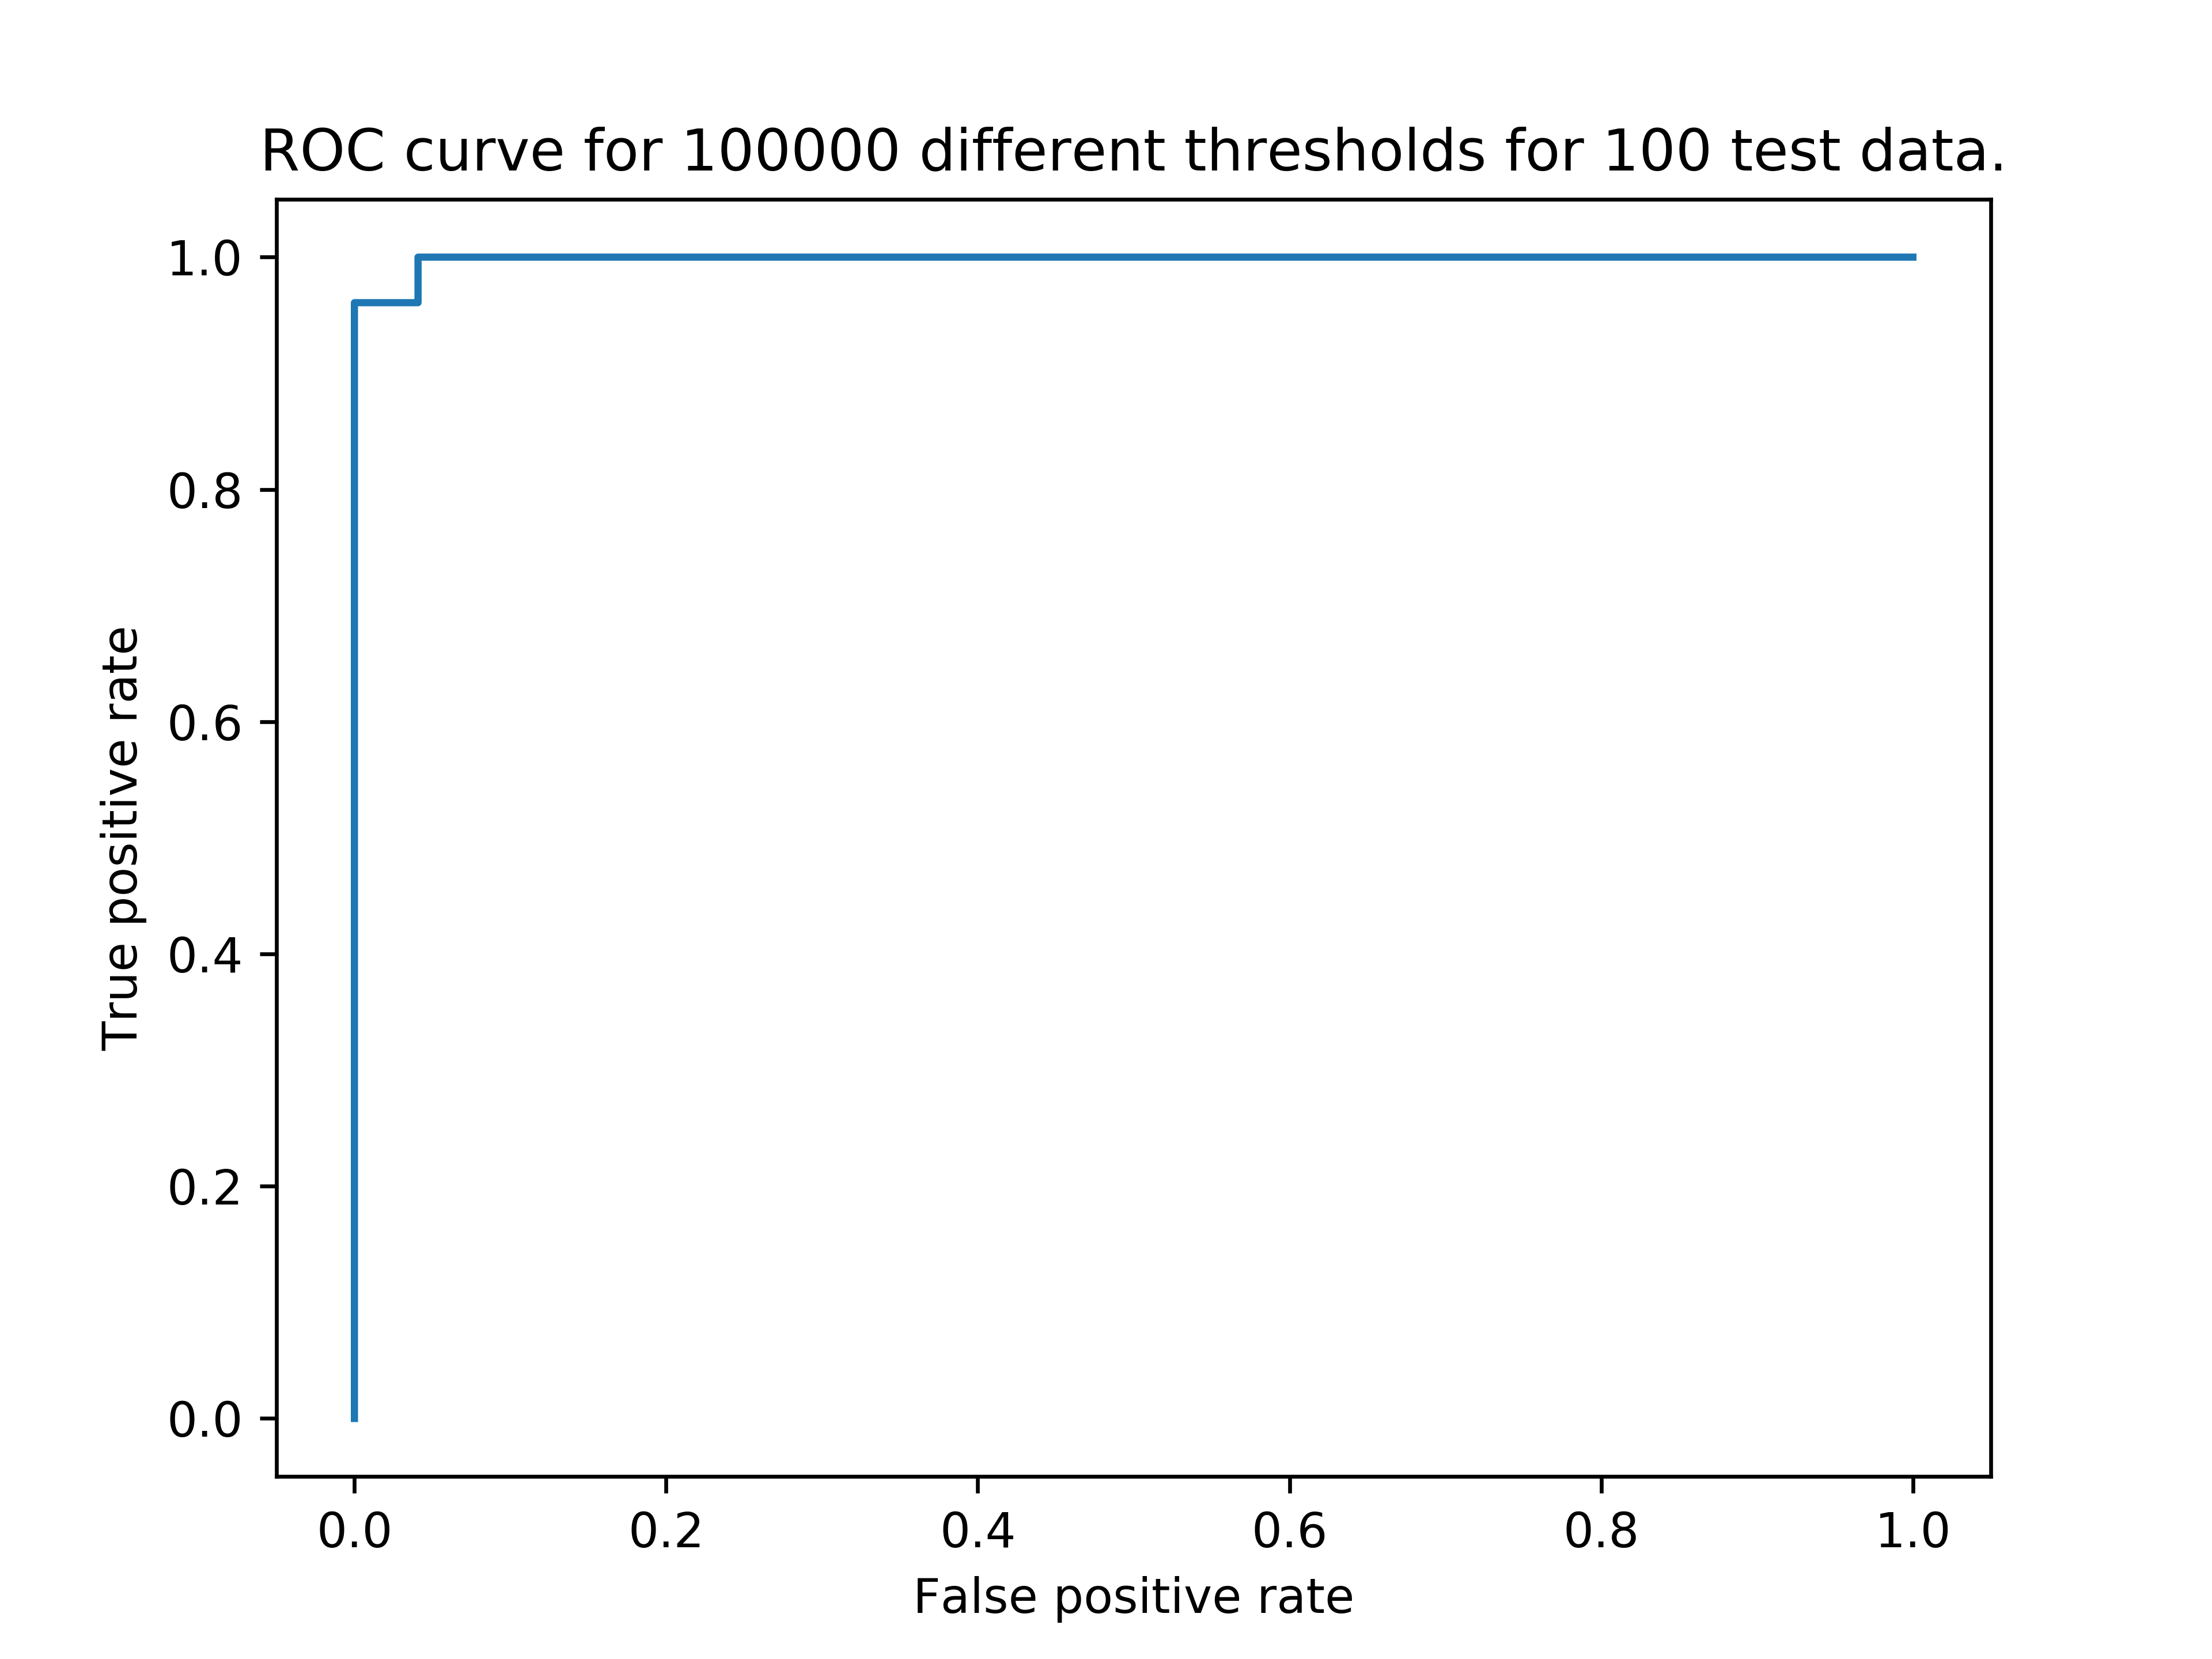
\includegraphics[scale=0.4]{figures/ROC_1.png}
%							\caption{\texttt{Area = 0.998399}}
%					\end{subfigure}
%					%
%					\begin{subfigure}[t]{0.6\textwidth}
%									\centering
%						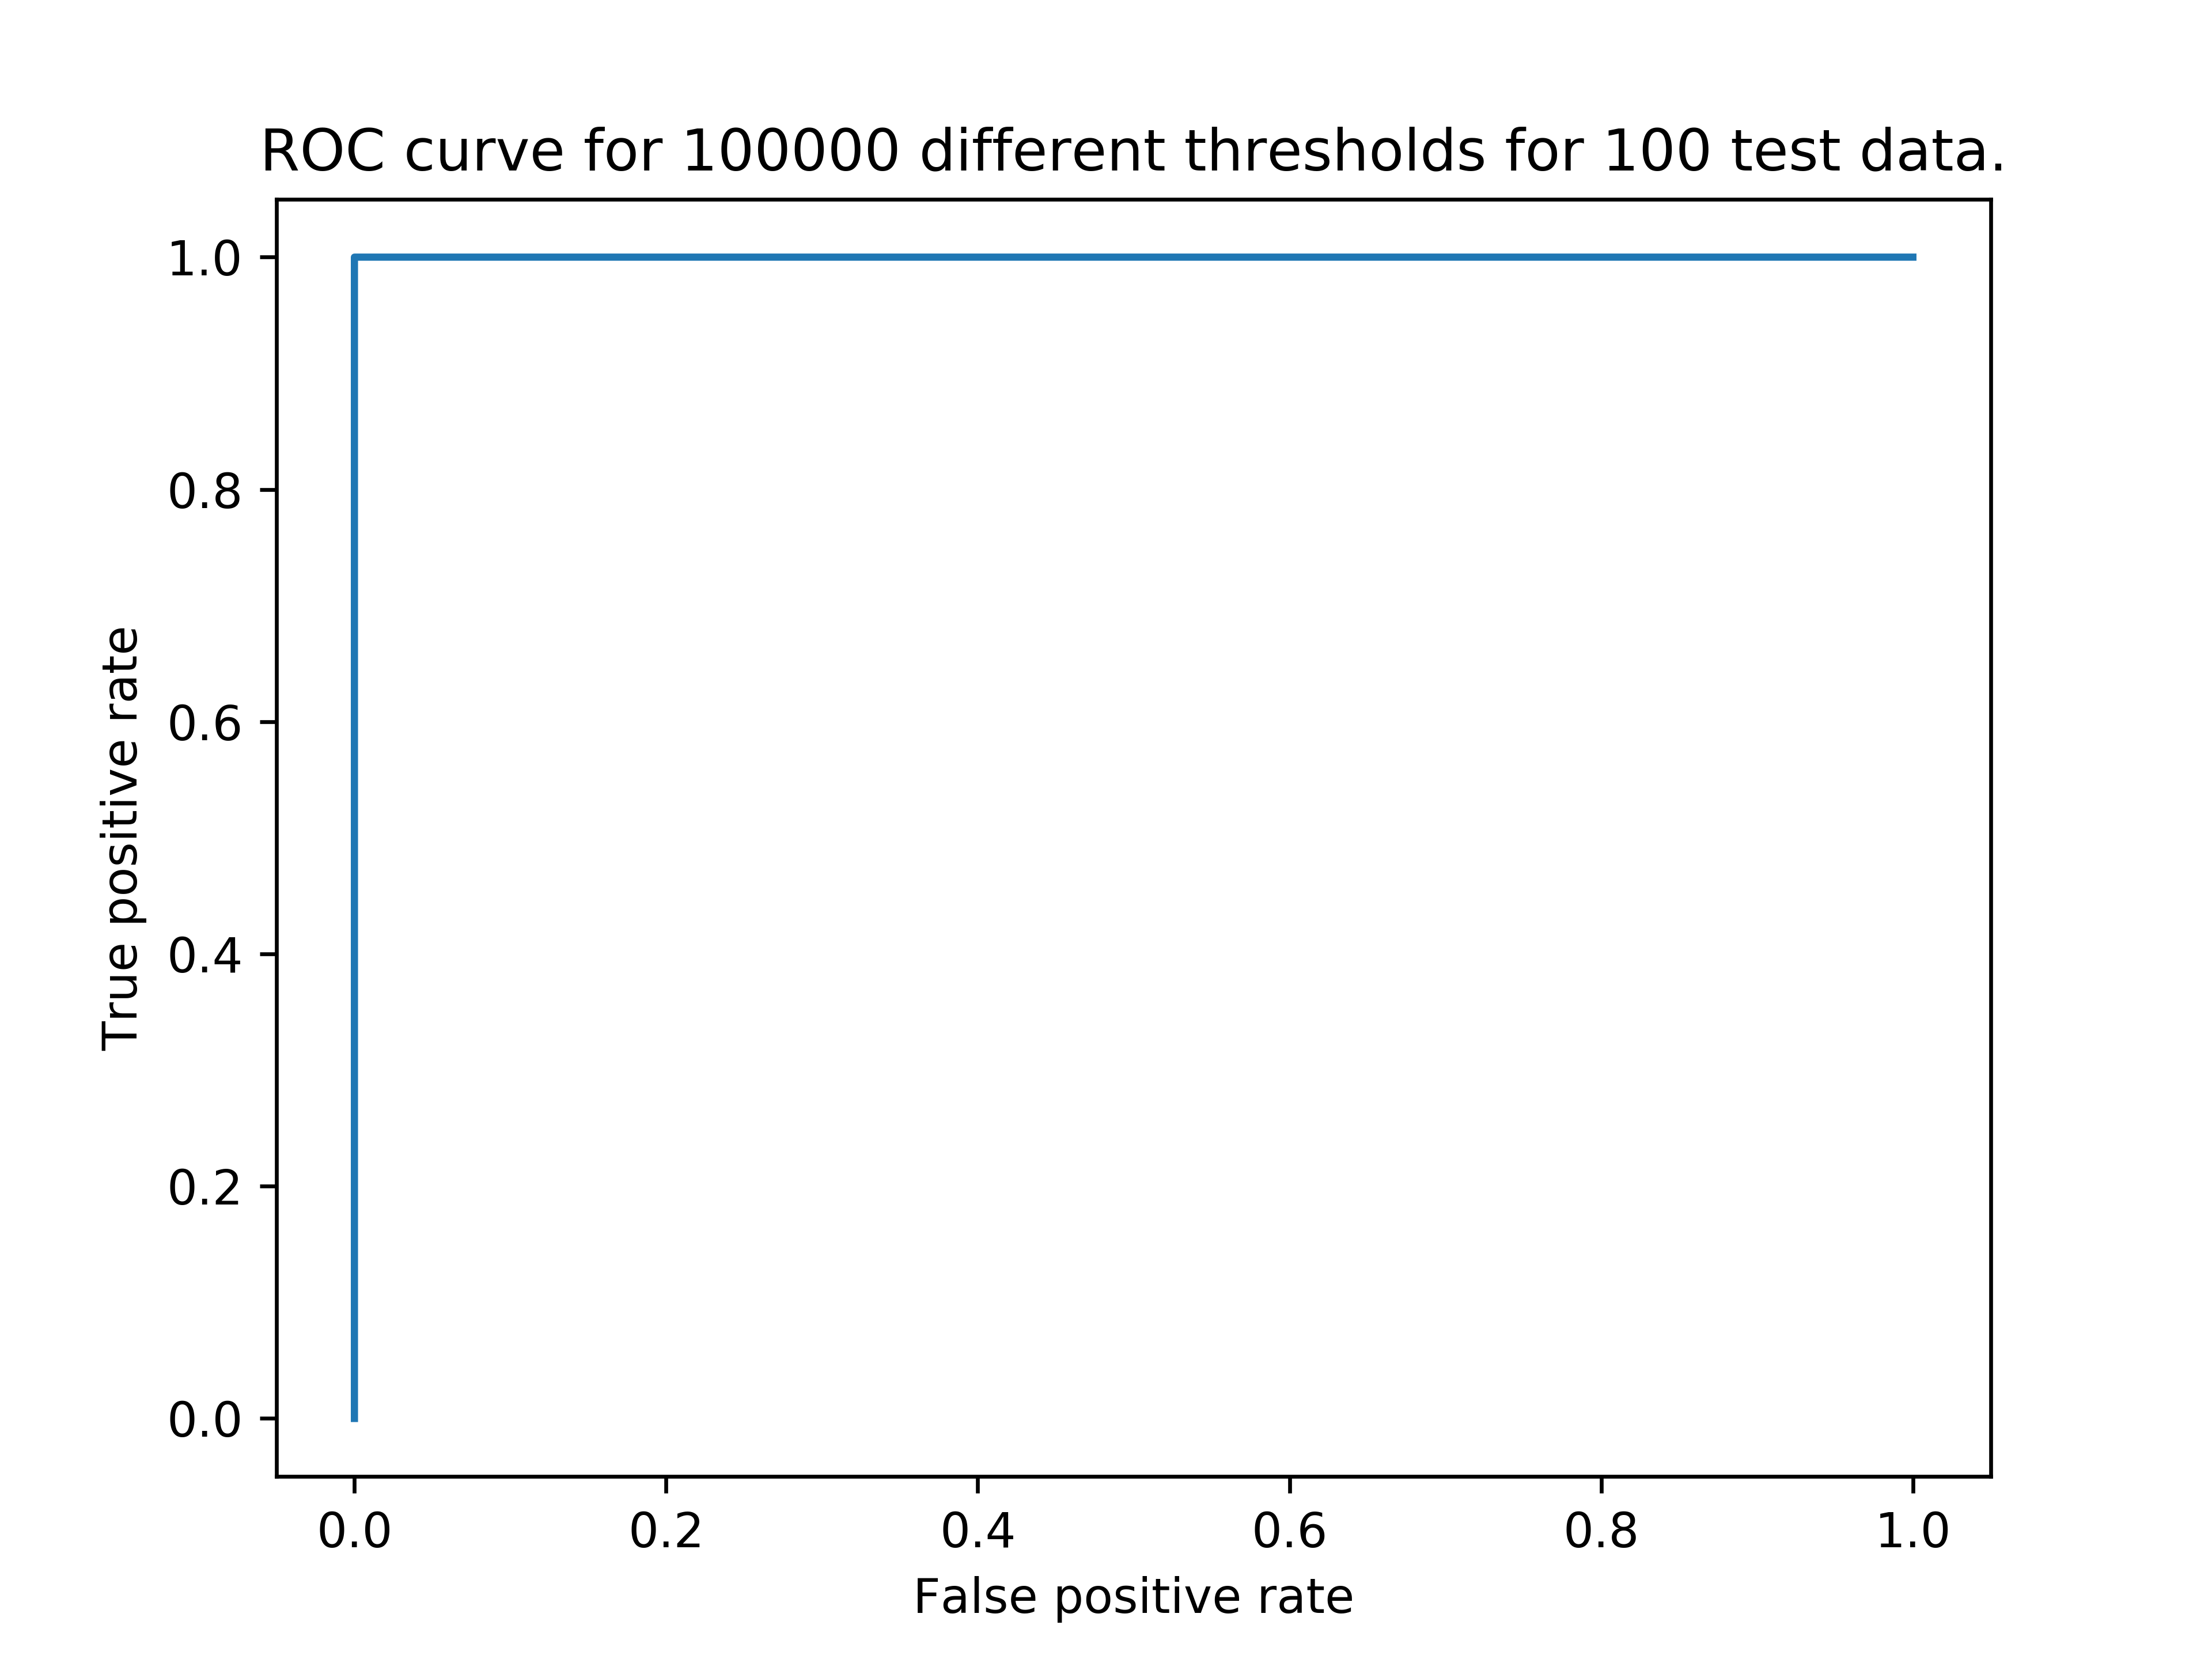
\includegraphics[scale=0.4]{figures/ROC_2.png}
%							\caption{\texttt{Area = 1.0}}						
%					\end{subfigure}
%					%
%					
%					\begin{subfigure}[t]{0.6\textwidth}
%									\centering
%						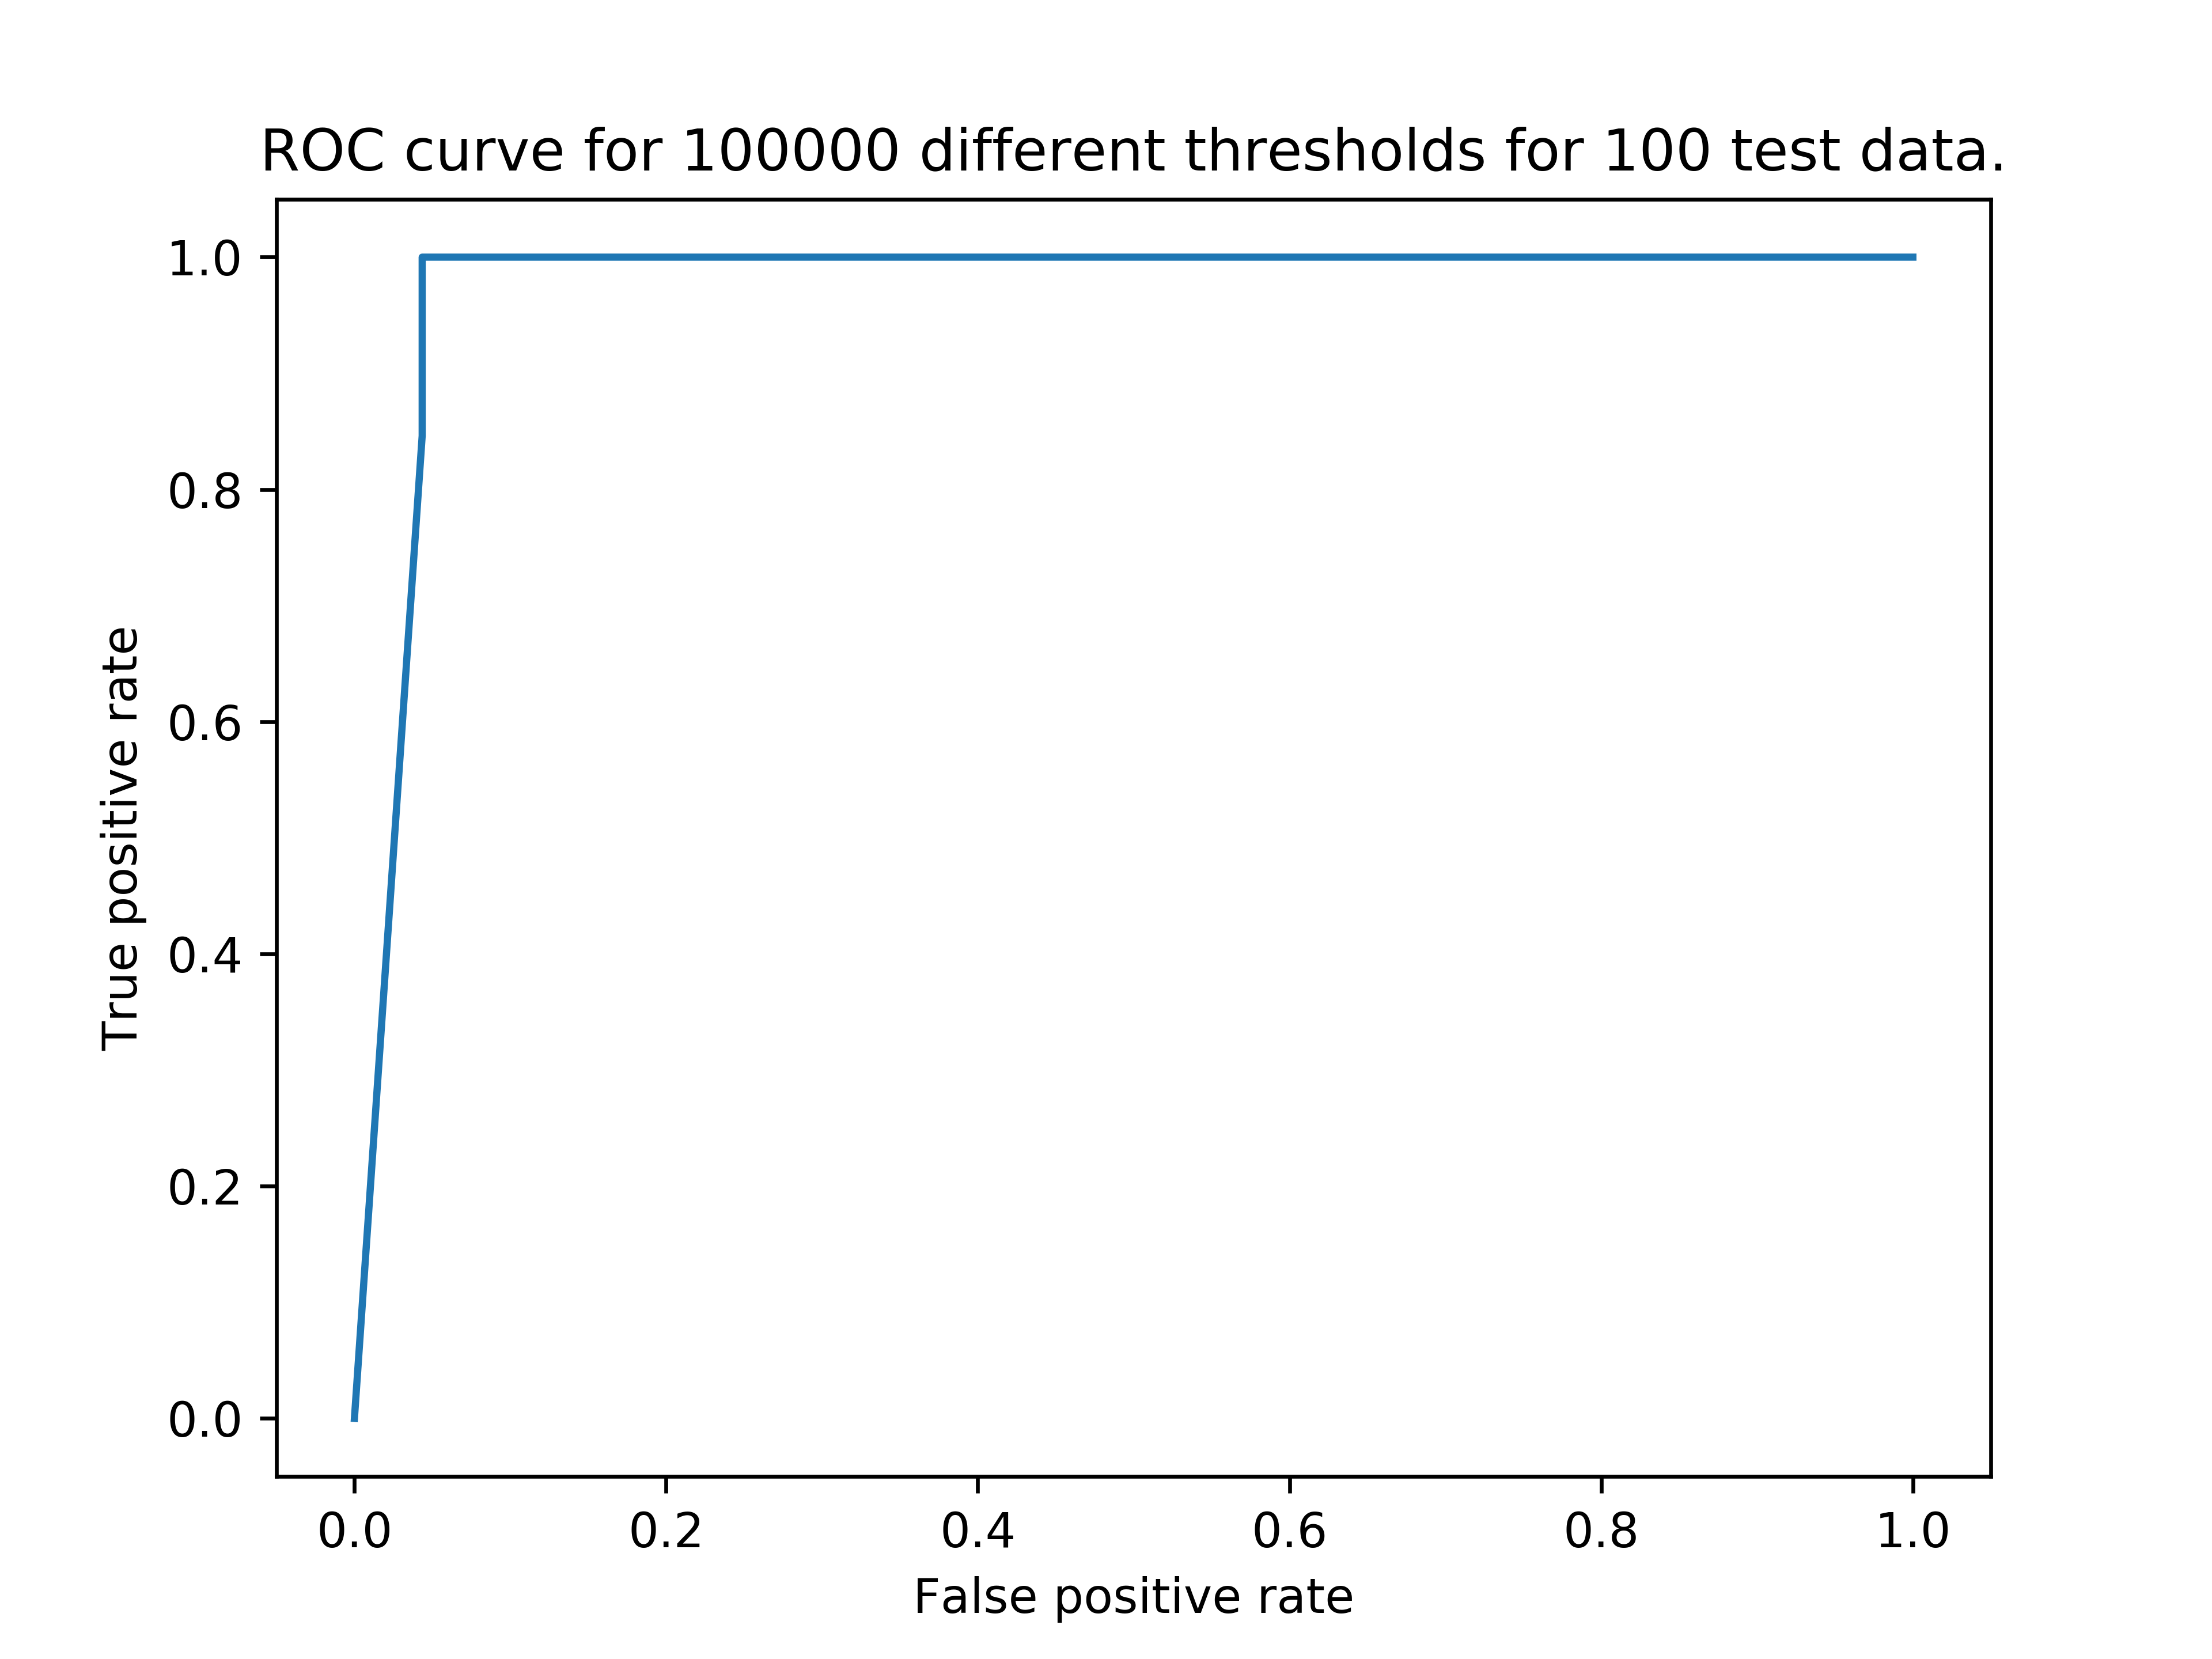
\includegraphics[scale=0.4]{figures/ROC_3.png}
%							\caption{\texttt{Area = 0.974916}}						
%					\end{subfigure}				
%					\caption{ROC curves for the same data as in Fig.s \ref{fig:test_plot_1}, \ref{fig:test_plot_2} and \ref{fig:test_plot_3}. The ROC curve represents, just like in the main test pool, correct positives to wrong negatives.}
%					\label{fig:multi_roc}			
%				\end{figure}

			
		\chapter{Conclusions}\label{Conclusions}
		
			Seen the results presented in Section \ref{network_results}, I can state that the objective of this thesis has been reached. I have managed to produce a Convolutional Neural Network which can distinguish, inside a timeseries from a satellite, the presence or not of a glitch with high accuracy. 
			
			In a real world application, such as a complete analysis of raw data from a satellite, the amount of information and scope can be far bigger than the one I have used. But the results I have obtained still show a successful applicability of Neural Network techniques to recognize glitches. 
			
			My hope is that this thesis might serve as a starting ground for future work on glitch recognition, especially in CMB bolometric missions, like \textbf{LiteBIRD}, and beyond.
		
%
%			BIBLIOGRAFIA
%
%\begin{thebibliography}{00}
\bibliography{citations/my_library}{}
\bibliographystyle{abbrv}
%
 
%\end{thebibliography}
% 

\end{document}
